\RequirePackage{pdfmanagement}
\SetKeys[document/metadata]{pdfversion=1.7, pdfstandard=A-2u, lang=en-GB}
\input{preamble/pdfA-compliance/glyphtounicode}
\documentclass[11pt,a4paper]{report}

\newcommand*{\PaperTitle}{The generalized Petlyuk arrangement minimizes total vaporization: a proof of the Halvorsen--Skogestad conjecture}
\newcommand*{\PaperTitlePlain}{The generalized Petlyuk arrangement minimizes total vaporization: a proof of the Halvorsen-Skogestad conjecture}
\newcommand*{\PaperShortTitle}{Proof of the Halvorsen--Skogestad conjecture}
\newcommand*{\PaperSubtitle}{chemistry-open-problems \textperiodcentered{} 20 October 2026 \textperiodcentered{} solved: lower bound and attainment independently verified by AI agents}
\newcommand*{\PaperCredits}{Mathematics, code and manuscript produced by AI agents, Claude Opus 5.5 (Anthropic) and GPT-6-Astra (OpenAI, via the Codex CLI), and independently verified by Claude Opus 5.5 agents. Detailed credits in the repository.}
\newcommand*{\PaperKeywords}{multicomponent distillation, Petlyuk arrangement, fully thermally coupled columns, dividing-wall columns, minimum vapor, minimum energy, Underwood equations, Vmin diagram, equilibrium-stage networks, M-matrices, perturbation theory}
\input{chemop-preamble}
\addbibresource{references.bib}
\usepackage{pgfplots}
\pgfplotsset{compat=1.18}

%% notation
\newcommand{\cA}{\mathcal A}
\newcommand{\cS}{\mathcal S}
\newcommand{\cC}{\mathcal C}
\newcommand{\cV}{\mathcal V}
\newcommand{\cW}{\mathcal W}
\newcommand{\cX}{\mathcal X}
\newcommand{\cJ}{\mathcal J}
\newcommand{\cL}{\mathcal L}
\newcommand{\cF}{\mathcal F}
\newcommand{\one}{\mathbf 1}
\newcommand{\bfe}{\mathbf e}
\newcommand{\Hs}{H^{*}}
\newcommand{\Spet}{\cS_{\mathrm{Pet}}}
\newcommand{\Ts}{\mathrm T}
\newcommand{\Bs}{\mathrm B}
\newcommand{\xb}{x_{\mathrm{bot}}}
\newcommand{\xt}{x_{\mathrm{top}}}
\newcommand{\bott}{\operatorname{bot}}
\newcommand{\topp}{\operatorname{top}}
\newcommand{\Maj}{\operatorname{Maj}}
\newcommand{\supp}{\operatorname{supp}}
\newcommand{\piv}{\varpi}
\newcommand{\Mm}{\mathbb M}
\newcommand{\Tm}{\mathbb T}

\begin{document}
\makepapertitle

\begin{paperabstract}
Halvorsen and Skogestad (Ind.\ Eng.\ Chem.\ Res.\ 2003) conjectured that, for an ideal feed (constant relative
volatilities, constant molar flows, constant pressure) separated into its pure components, with infinitely many stages
and no internal heat exchange, the generalized Petlyuk arrangement needs less vaporization than any other adiabatic
distillation arrangement, its minimum being the highest peak \(\max_jH_j\) of the \(V_{\min}\) diagram. We prove the
conjecture in a class \(\cA\) that contains every arrangement within their assumptions: all finite networks of
constant-molar-overflow equilibrium stages, single-phase splitters and mixers, total condensers and total vaporizers,
with one feed that may be split and conditioned, heat duties at any stage, recycles, and products of either phase.
Infinitely many stages and pure products enter as a limit of finite-stage steady states. The proof has two halves.
(i)~At every steady state of every arrangement of \(\cA\), with any numbers of stages, the total heat supplied
satisfies \(R\ge\sum_P\max(0,\varphi_P(\theta_j))\) for every root \(\theta_j\) of Underwood's feed equation, where
\(\varphi_P\) is the Underwood flux of the product stream \(P\); with product purities \(1-\varepsilon\) this gives
\(R\ge H_j-c_j\varepsilon\). The argument is elementary: all streams leaving an equilibrium stage have Underwood fluxes of
one sign, so the units split into a light and a heavy side, and the energy balance of the heavy side, in Underwood's
weights, gives the bound, with the excess as a sum of three nonnegative losses. (ii)~For every \(\delta>0\) and
\(\varepsilon>0\), the generalized Petlyuk arrangement with enough stages in every section has a steady state with all
purities at least \(1-\varepsilon\) and total vaporization \(\max_jH_j+\delta\). Its operating specification keeps every
column with three or more components close to its preferred split and forces a small flow of one key component into
each side product; in the infinite-stage limit every section is then pinched at one end only, the limit equations have
an invertible Jacobian (block triangular, with one triangular M-matrix per trace component), and the finite-stage
equations are an exponentially small perturbation of them. Hence the Petlyuk value of Halvorsen and Skogestad is the
exact minimum of the total vaporization over the whole class. All mathematics, code and text were produced by AI
agents, and every part was checked by independent AI verifiers.
\end{paperabstract}

\section{Introduction}\label{sec:intro}

\subsection{The conjecture}

The Petlyuk arrangement~\autocite{Petlyuk1965} and its realization as a dividing-wall column~\autocite{Kaibel1987}
are the best-known energy-saving devices of multicomponent distillation. Halvorsen and Skogestad analysed its minimum
energy for any number of components with Underwood's equations, introduced the \(V_{\min}\) diagram, and identified the
minimum vapor of the \emph{generalized} Petlyuk arrangement (one column for every set of consecutive components,
directly coupled; Figure~\ref{fig:petlyuk}) as the highest peak of that diagram~\autocite{HS1,HS2,HS3,HalvorsenThesis}. They then stated, in
the abstract of~\autocite{HS3}:
\begin{openquote}
``We also conjecture that the minimum energy requirement for the generalized extended Petlyuk arrangement is lower than
the minimum-energy requirement for any distillation configuration when we consider conventional adiabatic sections and
no internal heat exchange.''
\end{openquote}
Section~6.3 of~\autocite{HS3} (p.~626) makes the assumptions explicit:
\begin{openquote}
``We assume constant relative volatilities, constant molar flows, constant pressure, and no internal heat integration.
Then the generalized adiabatic Petlyuk arrangement has the lowest need for vaporization compared to any other adiabatic
distillation arrangement for separation of an arbitrary feed mixture into its pure components. We have not presented a
complete proof, so the above conclusion is a conjecture.''
\end{openquote}
The number of stages is infinite throughout~\autocite{HS3}. Even the minimum vapor of the Petlyuk arrangement itself was
established only in part (Section~5.3, p.~624):
\begin{openquote}
``We have not carried out a detailed proof for the general N-component M-product case for other than the far left and
right peaks.''
\end{openquote}
The conjecture was restated at Distillation \& Absorption 2002~\autocite{HS02}, where infinitely many stages are
assumed ``because this provides a lower bound on the energy requirement'' for ideal mixtures and the energy is measured
by the total vaporization. In this paper we prove it, together with the formula for the Petlyuk minimum, for every
number of components.

\subsection{What was known}

For three components, Fidkowski and Kr\'olikowski~\autocite{FK87} compared the Petlyuk column in closed form with side
strippers, side rectifiers and the direct and indirect sequences; Halvorsen reports Petlyuk's statement that ``no proof
has been found in the literature, except for the ternary case''~\autocite[\S6]{HS3}. For four or more components the
property has been tested, not proved: Underwood-model enumerations and global optimization of the space of
regular-column configurations~\autocite{SA10,Nallasivam2016,TGAT} find the fully thermally coupled (FTC, generalized
Petlyuk) value optimal on the instances solved, Fidkowski and Agrawal~\autocite{FA01} and Fidkowski~\autocite{Fidkowski2006}
note that no rigorous proof is available, and a 2021 thesis from the same group states that ``for four and more components,
the conjecture is yet to be proved or disproved''~\autocite[p.~125]{MathewThesis}, after proving it for one
four-component family by a vapor balance on a suitably chosen boundary. Some later papers describe the property as
established~\autocite{HS2011,NavarroAmoros2013,CaballeroGrossmann2014}; they refer back to~\autocite{HS3}, which calls
it a conjecture.

The ingredients of our lower bound are classical when used one section at a time. Underwood's identity between
consecutive stages holds for a free parameter~\autocite{Underwood1948},\autocite[eqs.~(2.45)--(2.49)]{HalvorsenThesis}; Franklin
and Forsyth used the signs of Underwood coordinates inside one column~\autocite{FranklinForsyth1953}; stage-level sign
comparisons of an Underwood-type function inside one section of a multi-feed column prove convergence to a
pinch in~\autocite[Prop.~5.4.1]{JiangThesis} and~\autocite[Prop.~1]{Jiang2022}; and cut or vapor-balance arguments at the
common roots were used for one arrangement (the equality case of the Petlyuk arrangement~\autocite[\S3]{HS3}), one
junction~\autocite[\S6.2.1]{HalvorsenThesis} and one four-component family~\autocite[\S6.3]{MathewThesis}. We found no work
that combines them over a whole network. For attainment, the finite-stage behaviour of Petlyuk columns has been studied by
simulation~\autocite{HS1999,MalinenTanskanen2007},\autocite[\S5.2.7]{HalvorsenThesis}, which confirms numerically that
finite-stage operation approaches the Underwood values, and the theory of single sections and columns with constant
volatilities is classical~\autocite{Underwood1948,FranklinForsyth1953,AcrivosAmundson1955,PetlyukBook}; we found no proof that
steady states of a closed, thermally coupled network converge to the Underwood configuration.

Two difficulties stand in the way of a proof. First, ``any distillation configuration'' is not a finite list:
besides the regular-column configurations~\autocite{Agrawal2003,SA10} it includes columns with several feed stages,
stream splitters, remixing, recycles, bypasses, and operation with reverse net flows. Second, the infinite-stage
Underwood model in which minimum vapor is computed is itself an idealization, and the formulations used for
optimization are relaxations whose feasible points need not be limits of physical operation; we show in
Remark~\ref{rem:permissive} that one such formulation admits a five-component point below the Petlyuk value.
We therefore work in the physical model: networks of equilibrium stages with finitely many stages, of which
``infinitely many stages and pure products'' is a limit.

\subsection{Results}

Let \(\alpha_1>\dots>\alpha_N>0\) be the relative volatilities, \(z\) the feed composition (\(z_p>0\),
\(\sum_pz_p=1\)), \(q\in\R\) the liquid fraction of the feed (feed flow \(1\)), \(\theta_j\in(\alpha_{j+1},\alpha_j)\) the
roots of Underwood's feed equation \(\sum_p\alpha_pz_p/(\alpha_p-\theta)=1-q\), and
\[H_j=\sum_{p>j}\frac{\alpha_pz_p}{\theta_j-\alpha_p}\qquad(j=1,\dots,N-1),\qquad \Hs=\max_jH_j ,\]
the peaks of the \(V_{\min}\) diagram referred to the reboiler (Section~\ref{sec:data}). For a family \(\cS\) of
arrangements, \(R^*(\cS)\) denotes the limit, as \(\varepsilon\to0\), of the infimum of the total vaporization \(R\) over
the steady states of members of \(\cS\) whose products all have purity at least \(1-\varepsilon\)
(Definition~\ref{def:limit}); \(\Spet\) is the generalized Petlyuk arrangement with all possible numbers of stages.

\begin{theorem}[main theorem]\label{thm:main}
Let \(\cA\) be the class of Definition~\ref{def:A}.
\begin{enumerate}
\item (Lower bound.) At every steady state of every arrangement of \(\cA\) whose products all have purity at least
\(1-\varepsilon\), \(R\ge H_j-c_j\varepsilon\) for every \(j\), with
\(c_j=\max\bigl(\alpha_j/(\alpha_j-\theta_j),\,\alpha_{j+1}/(\theta_j-\alpha_{j+1})\bigr)\). Hence \(R^*(\cS)\ge\Hs\) for
every family \(\cS\subseteq\cA\).
\item (Attainment.) For every \(\delta>0\) and \(\varepsilon>0\) there is \(n_0\) such that the generalized Petlyuk
arrangement with at least \(n_0\) stages in every section has an operating specification with total heat supply
\(R=\Hs+\delta\) and a steady state at which every mole fraction is positive and every product has purity at least
\(1-\varepsilon\). Hence \(R^*(\Spet)=\Hs\).
\item (The conjecture.) \(R^*(\cS)\ge R^*(\Spet)=\Hs\) for every family \(\cS\subseteq\cA\): no arrangement of \(\cA\)
needs less total vaporization, with infinitely many stages and pure products, than the generalized Petlyuk
arrangement, whose minimum is the highest peak of the \(V_{\min}\) diagram.
\end{enumerate}
\end{theorem}

Part~1 is Theorem~\ref{thm:stage} and Corollary~\ref{cor:purity}; part~2 is Theorem~\ref{thm:attain}
(Proposition~\ref{prop:binary} for \(N=2\)); part~3 is Corollary~\ref{cor:conjecture}. ``Lowest'' in the conjecture
must be read as ``lowest or equal'': many arrangements tie with the Petlyuk value~\autocite[\S7]{HS3},\autocite{Jiang2018}.

\emph{The lower bound} rests on one observation. Define the \emph{Underwood flux} of a stream with vapor flow \(v\) and
component flows \(n_i\) as \(\varphi(\theta)=v-\sum_i\alpha_in_i/(\alpha_i-\theta)\). Under constant molar overflow, the
fluxes are conserved at every unit up to its heat duty; at \(\theta=\theta_j\) the feed carries no flux; and every stream
leaving an equilibrium stage, liquid or vapor, has a flux of the sign of \(-\sum_i\alpha_ix_i/(\alpha_i-\theta_j)\), where
\(x\) is the stage liquid. The units therefore split into a light and a heavy side, and the energy balance of the heavy
side gives the bound, whatever the topology, the number of stages, the signs of the net flows or the purities
(Section~\ref{sec:bound}). The excess of \(R\) over the bound is an explicit sum of three nonnegative ``pinch losses'',
which yields necessary conditions for an arrangement to tie with the Petlyuk value.

\emph{Attainment} is harder. In Underwood's infinite-stage model, Halvorsen and Skogestad's construction (every internal
column at its preferred split) reaches \(\Hs\)~\autocite{HS3}. The difficulty is to show that finite-stage steady states
of the closed, thermally coupled network converge to it. Two obstacles appear. If the binary columns are operated with
both products sharp, the limit equations have a kernel: the composition of the feed stage of every binary column is not
determined in the limit (a ``neutral mode''), and the finite-stage solutions are then fixed only by exponentially small
terms. And at the exact Petlyuk minimum several sections are pinched at both ends. We avoid both by an operating
specification (Section~\ref{sec:design}) that keeps a margin \(\delta\) in the reboiler, deforms every column with three
or more components slightly away from its preferred split in a direction that preserves its common Underwood roots, and
\emph{forces} every binary column by sending a small prescribed flow of one key component into the adjacent side product.
In the infinite-stage limit every section is then pinched at one end only, and the limit equations in the unknowns
``junction compositions and column splits'' have an invertible Jacobian, with a block-triangular structure: one
top-down block for the major components (Underwood interpolation and a Cauchy-type matrix in every column) and one
triangular M-matrix for every component present only in traces (Theorem~\ref{thm:L}). The finite-stage equations
differ from the limit equations by terms of size \(\rho^{n}\) in \(C^1\), so a quantitative inverse-function argument
gives a finite-stage steady state near the limit for all section lengths \(\ge n_0\), and an M-matrix argument shows
that all its mole fractions are positive (Section~\ref{sec:analysis}). The limits are taken in the order
\(n\to\infty\), then forcing \(\to0\), then \(\delta\to0\).

\subsection{Outline}

Section~\ref{sec:model} defines the class \(\cA\), the limit \(R^*\), and their relation to Underwood's model.
Section~\ref{sec:bound} proves the lower bound and discusses its consequences. Section~\ref{sec:attain} states
finite-stage attainment, proves it for two components, and gives the construction and the statements of the proof for
\(N\ge3\); the proofs are in Appendices~\ref{app:section}--\ref{app:analysis}. Section~\ref{sec:numerics} illustrates
the attainment theorem numerically, and Section~\ref{sec:discussion} discusses scope, limitations and open questions.
Appendix~\ref{app:repro} lists the computations that check the statements (none is used in a proof).

\section{Model}\label{sec:model}

\subsection{Data, feed roots and peaks}\label{sec:data}

There are \(N\ge2\) components with constant relative volatilities \(\alpha_1>\alpha_2>\dots>\alpha_N>0\), so that a vapor in
equilibrium with a liquid of composition \(x\) has the composition
\[y(x)=\frac{\diag(\alpha)\,x}{S(x)},\qquad S(x)=\sum_k\alpha_kx_k .\]
The pressure is constant, molar flows are constant (constant molar overflow, CMO), and the molar heat of vaporization is
the unit of heat, so that heat duties are measured in moles of vapor generated. The process feed has flow \(1\), composition
\(z\) (all \(z_p>0\)) and liquid fraction \(q\in\R\) (\(q>1\) subcooled, \(q<0\) superheated): it brings the vapor
equivalent \(1-q\). The function \(t\mapsto\sum_p\alpha_pz_p/(\alpha_p-t)\) increases from \(-\infty\) to \(+\infty\) on every
interval \((\alpha_{j+1},\alpha_j)\), so Underwood's feed equation
\begin{equation}\label{eq:feedroots}
\sum_{p=1}^N\frac{\alpha_pz_p}{\alpha_p-\theta}=1-q
\end{equation}
has exactly one root \(\theta_j\in(\alpha_{j+1},\alpha_j)\) for each \(j=1,\dots,N-1\), for every \(q\). The \emph{peaks}
\(H_j\) and \(\Hs\) are defined above; we also write \(g_j:=\Hs-H_j\ge0\). \(H_j\) is the minimum boilup of a two-product column
that splits the feed sharply between components \(j\) and \(j+1\) (Underwood's formula at the active root \(\theta_j\)): the
peak \(P_{j,j+1}\) of the \(V_{\min}\) diagram~\autocite{HS1}, referred to the reboiler. Referred to the top, the peaks are
\(H_j+1-q=\sum_{p\le j}\alpha_pz_p/(\alpha_p-\theta_j)\). We write \(G_x(t)=\sum_i\alpha_ix_i/(\alpha_i-t)\) for Underwood's
function of a composition (or of any vector) \(x\), \(\one\) for the all-ones vector, \(\bfe_p\) for the \(p\)-th unit vector
and \(\cX=\{x\in\R^N:x\ge0,\ \one^\top x=1\}\) for the simplex of compositions.

\subsection{The class of arrangements}\label{sec:classA}

Halvorsen's thesis (\S6.1.1 of~\autocite{HalvorsenThesis}) describes an arrangement as sections of connected equilibrium
stages, reboilers and condensers, directly coupled by two-way liquid and vapor streams or coupled through condensers or
reboilers, divided at stages with feed or side-draw streams; under CMO the energy balance of every stage reduces to
``vapor out minus vapor in equals heat input'' (\emph{ibid.}, \S2.6.1). The following definition keeps exactly these
physical ingredients and drops every restriction on how they are connected.

\begin{definition}[the class \(\cA\)]\label{def:A}
An \emph{arrangement} is a finite directed multigraph whose vertices are \emph{units} and whose arcs are
\emph{streams}, together with a feed source and product outlets. A stream \(e\) has a phase (saturated liquid or saturated
vapor), component flows \(n_{e,i}\ge0\) and vapor flow \(v_e\) (\(=\sum_in_{e,i}\) for a vapor, \(0\) for a liquid). The
units are of four types:
\begin{itemize}
\item[(E)] \emph{equilibrium stage}: any inflows; an external heat duty \(Q_u\in\R\); its contents leave as a liquid of
composition \(x_u\) and a vapor of composition \(y(x_u)\), each divided into any number of outflow streams (either phase may
have zero flow);
\item[(M)] \emph{single-phase mixer or splitter}: inflows of one phase, outflows of that phase and of the mixed
composition, \(Q_u=0\);
\item[(C)] \emph{total condenser}: vapor inflows, liquid outflows of the mixed composition;
\item[(R)] \emph{total vaporizer}: liquid inflows, vapor outflows of the mixed composition.
\end{itemize}
The process feed is divided into portions of sizes \(f_u\ge0\), \(\sum_uf_u=1\), each entering an (E) unit with the
feed's composition and thermal state (feed conditioning is an (E) unit with a duty). Every stream leaving the arrangement is a \emph{product stream} and is assigned to one
component. A \emph{steady state} is an assignment of flows and compositions such that at every unit \(u\)
\begin{equation}\label{eq:balances}
\sum_{e\text{ out of }u}n_{e,i}-\sum_{e\text{ into }u}n_{e,i}=f_uz_i\quad(\text{all }i),\qquad
\sum_{e\text{ out of }u}v_e-\sum_{e\text{ into }u}v_e=Q_u+(1-q)f_u ,
\end{equation}
product streams counting as outflows, and the composition rule of its type holds (this defines \(Q_u\) for (C) and (R)
units). Its \emph{total vaporization} is \(R=\sum_u\max(Q_u,0)\), the total heat supplied.
\end{definition}

Nothing is assumed on the topology (recycles are cycles of the graph), on the signs of the net component flows, on which
components are present where, on the numbers of stages, or on the stability or uniqueness of steady states. An
\emph{adiabatic section} is a chain of (E) units with \(Q=0\), liquid flowing down and vapor flowing up with constant flows;
a column is a stack of sections joined at junction stages.

\emph{What \(\cA\) contains.} Every device of the arrangements considered
in~\autocite{HS3,HalvorsenThesis,Agrawal2003,Fidkowski2006,SA10,TGAT,CSL97} is a sub-network of units of \(\cA\), with
the same balances and the same compositions of every stream that leaves it: conventional columns with total or partial
condensers and reboilers; thermal couplings; side draws of either phase; side strippers and rectifiers; Petlyuk,
generalized Petlyuk and Kaibel arrangements and dividing-wall columns (a liquid or vapor split is a stage outflow divided
into several streams, a merge is several inflows into one stage); several feed stages per column and intermediate
sections; stream splitters dividing a section product among several columns, remixing, vapor or liquid bypasses (tray
entrainment and weeping included), recycles; feed splitting, preheating, precooling and pre-flashing; intermediate
reboilers and condensers, heaters and coolers at any stage, that is, non-adiabatic sections with external utilities
(which the conjecture does not require us to admit); and trays with a Murphree vapor efficiency \(E\in[0,1]\) common to all
components, which are exactly an (E) unit receiving the fraction \(E\) of the vapor from below, a vapor bypass of the
fraction \(1-E\) and an (M) mixer; cross-flow trays (whose Murphree efficiency may exceed one) are liquid cells in series,
each contacted by a portion of the vapor. Partial condensation or vaporization giving two phases of the same composition
is an (M) splitter followed by a (C) or (R) unit. Differential condensation or vaporization, and rate-based contacting with
component-independent film coefficients, are limits of members of \(\cA\), to which the bound below passes by continuity.

\emph{What \(\cA\) excludes, and why the conjecture excludes it.} Heat exchange between process streams that is not counted
in \(R\) (``internal heat exchange'', excluded in~\autocite[\S6.3, \S8]{HS3}; it lowers the external heat below the
Petlyuk value~\autocite[Table~6.1]{HalvorsenThesis}); a well-mixed tray with a Murphree efficiency above one (unphysical);
several pressures (excluded by constant pressure; they act through
heat exchange between columns or compression and change \(\alpha\)); non-ideal mixtures and non-CMO enthalpies; devices that
release streams of different compositions not in phase equilibrium (decanters, membranes, component-dependent stage
efficiencies or mass-transfer coefficients); heat pumps; several process feeds of different compositions or thermal
states; and non-steady (batch or cyclic) operation. Finite stages and impure products are not excluded: they are the
objects of the model.

\subsection{Infinitely many stages and pure products}\label{sec:limit}

\begin{definition}[the limit of infinitely many stages and pure products]\label{def:limit}
A steady state has \emph{purity at least \(1-\varepsilon\)} if every product stream assigned to a component \(p\) has mole
fraction of \(p\) at least \(1-\varepsilon\). For a family \(\cS\subseteq\cA\) (for example all stage numbers of one
configuration, or all of \(\cA\)) put
\begin{gather*}
R^*(\cS;\varepsilon)=\inf\{R(s):s\text{ a steady state of a member of }\cS\text{, purity at least }1-\varepsilon\},\\
R^*(\cS)=\lim_{\varepsilon\to0^+}R^*(\cS;\varepsilon).
\end{gather*}
\end{definition}
The limit exists in \([0,+\infty]\) because \(R^*(\cS;\varepsilon)\) is nonincreasing in \(\varepsilon\). For a configuration
\(X\) (a topology with unspecified numbers of stages), \(R^*(\cS_X)\), with \(\cS_X\) the arrangements of topology \(X\) and
any numbers of stages, is the faithful meaning of ``the minimum vapor of \(X\) with infinitely many stages and pure
products'': every real arrangement has finitely many stages and impure products, and infinite-stage values are used,
in the words of~\autocite{HS02}, because they provide a lower bound on the energy requirement. In this language:

\begin{definition}[the Halvorsen--Skogestad conjecture in \(\cA\)]\label{def:conj}
\(R^*(\Spet)\le R^*(\cS)\) for every family \(\cS\subseteq\cA\), and \(R^*(\Spet)=\Hs\) (the formula of~\autocite{HS3} for
the Petlyuk minimum).
\end{definition}

\emph{Relation to Underwood's model.} In Underwood's infinite-stage model each section is described by its flows and net
component flows, and its compositions at the ends are its pinch compositions; the minimum vapor of a configuration is
then a finite-dimensional optimization problem~\autocite{HS3,Nallasivam2016,TGAT}. Definition~\ref{def:limit} does not
use this model. Theorem~\ref{thm:main} shows that for the generalized Petlyuk arrangement the two notions agree
(\(R^*(\Spet)\) equals Halvorsen and Skogestad's Underwood value), and that no arrangement can do better in the physical
sense. Underwood-model formulations used for global optimization are best seen as relaxations: their points need not be
limits of physical steady states, and one of them admits points below \(\Hs\) (Remark~\ref{rem:permissive}).

\section{The lower bound}\label{sec:bound}

\subsection{The Underwood flux and the cut theorem}

For \(\theta>0\), \(\theta\notin\{\alpha_i\}\), the \emph{Underwood flux} of a stream \(e\) and of a unit of feed are
\begin{equation}\label{eq:flux}
\varphi_e(\theta)=v_e-\sum_i\frac{\alpha_in_{e,i}}{\alpha_i-\theta},\qquad
\varphi_F(\theta)=(1-q)-\sum_i\frac{\alpha_iz_i}{\alpha_i-\theta},
\end{equation}
so that \(\varphi_F(\theta_j)=0\) for every \(j\) by~\eqref{eq:feedroots}. For the same component flows, a vapor stream has
the flux of the liquid stream plus its total flow.

\begin{lemma}[node balance]\label{lem:node}
At every unit \(u\) of a steady state and for every \(\theta>0\), \(\theta\notin\{\alpha_i\}\),
\[\sum_{e\text{ out of }u}\varphi_e(\theta)-\sum_{e\text{ into }u}\varphi_e(\theta)=Q_u+f_u\varphi_F(\theta).\]
\end{lemma}
\begin{proof}
\(\varphi_e=v_e-\sum_ic_in_{e,i}\) with \(c_i=\alpha_i/(\alpha_i-\theta)\) is linear in \((v_e,n_e)\). Subtract \(\sum_ic_i\) times the
component balances from the energy balance in~\eqref{eq:balances}.
\end{proof}

\begin{lemma}[sign uniformity]\label{lem:uniform}
Let \(\theta>0\), \(\theta\notin\{\alpha_i\}\). A liquid stream of flow \(l\) and composition \(x\) has
\(\varphi=-l\,G_x(\theta)\); a vapor stream of flow \(v\) in equilibrium with a liquid of composition \(x\) has
\(\varphi=-(\theta v/S(x))\,G_x(\theta)\). Hence all streams leaving an (E) unit have fluxes of one sign, that of
\(-G_{x_u}(\theta)\), and so do all streams leaving an (M), (C) or (R) unit.
\end{lemma}
\begin{proof}
For the vapor, with \(\sum_iy_i=1\), \(y_i=\alpha_ix_i/S(x)\) and \(\alpha_i/(\alpha_i-\theta)=1+\theta/(\alpha_i-\theta)\):
\(\varphi=v\sum_iy_i\bigl(1-\frac{\alpha_i}{\alpha_i-\theta}\bigr)=-\theta v\sum_i\frac{y_i}{\alpha_i-\theta}=-\frac{\theta v}{S(x)}G_x(\theta)\), and
\(\theta>0\), \(S(x)>0\). The outflows of an (M), (C) or (R) unit have one phase and one composition, so their fluxes are
nonnegative multiples of one number.
\end{proof}

Fix \(j\) and \(\theta=\theta_j\). Call a unit \emph{heavy-ish} if all its outflows have \(\varphi(\theta_j)\ge0\) and
\emph{light-ish} otherwise; by Lemma~\ref{lem:uniform} all outflows of a light-ish unit have \(\varphi(\theta_j)\le0\). Let
\(\mathcal U_+\), \(\mathcal U_-\) be the two sets of units, \(R(\mathcal W)=\sum_{u\in\mathcal W}\max(Q_u,0)\) and
\(Q(\mathcal W)=\sum_{u\in\mathcal W}\max(-Q_u,0)\).

\begin{theorem}[stage-level cut]\label{thm:stage}
At every steady state of every arrangement of \(\cA\), with any numbers of stages and any purities, and for every \(j\),
\begin{equation}\label{eq:defect}
R-\sum_P\max\bigl(0,\varphi_P(\theta_j)\bigr)=R(\mathcal U_-)+Q(\mathcal U_+)
+\sum_{e\colon\mathcal U_+\to\mathcal U_-}\varphi_e(\theta_j)-\sum_{e\colon\mathcal U_-\to\mathcal U_+}\varphi_e(\theta_j),
\end{equation}
the first sum running over the product streams and the last two over the streams between the two sets; every term on
the right is nonnegative. In particular \(R\ge\sum_P\max(0,\varphi_P(\theta_j))\).
\end{theorem}
\begin{proof}
Sum Lemma~\ref{lem:node} over \(u\in\mathcal U_+\) at \(\theta_j\), where the feed terms vanish. Streams with both ends in
\(\mathcal U_+\) cancel, so
\(R(\mathcal U_+)-Q(\mathcal U_+)=\sum_{P\text{ from }\mathcal U_+}\varphi_P+\sum_{\mathcal U_+\to\mathcal U_-}\varphi_e-\sum_{\mathcal U_-\to\mathcal U_+}\varphi_e\).
Product streams leaving \(\mathcal U_+\) have \(\varphi_P\ge0\) and those leaving \(\mathcal U_-\) have \(\varphi_P\le0\), so the first
sum is \(\sum_P\max(0,\varphi_P)\); streams leaving \(\mathcal U_+\) have \(\varphi\ge0\) and streams leaving \(\mathcal U_-\) have
\(\varphi\le0\), so the crossing terms are nonnegative. Add \(R(\mathcal U_-)+Q(\mathcal U_+)\) to both sides and use
\(R=R(\mathcal U_+)+R(\mathcal U_-)\).
\end{proof}

\begin{corollary}[pure products]\label{cor:pure}
If every product stream is pure, then \(R\ge H_j\) for every \(j\), that is, \(R\ge\Hs\).
\end{corollary}
\begin{proof}
A pure liquid product of component \(p\) and flow \(P\) has \(\varphi=\alpha_pP/(\theta_j-\alpha_p)\), a pure vapor product
\(\varphi=\theta_jP/(\theta_j-\alpha_p)\); both are positive exactly when \(p>j\), the vapor value being the larger. The products
of component \(p\) carry \(z_p\) in total.
\end{proof}

\begin{corollary}[finite purity]\label{cor:purity}
If every product stream has purity at least \(1-\varepsilon\), then \(R\ge H_j-c_j\varepsilon\) for every \(j\), with \(c_j\) as in
Theorem~\ref{thm:main}. Consequently \(R^*(\cS)\ge\Hs\) for every family \(\cS\subseteq\cA\).
\end{corollary}
\begin{proof}
Since a vapor stream has the flux of the liquid stream with the same component flows plus its total flow, it suffices to
bound liquid fluxes from below. Keeping only the products assigned to components \(p>j\),
\(\sum_P\max(0,\varphi_P)\ge\sum_{i>j}\alpha_in^h_i/(\theta_j-\alpha_i)-\sum_{i\le j}\alpha_in^h_i/(\alpha_i-\theta_j)\), where \(n^h_i\)
is the flow of \(i\) in these products. By the overall balance, \(n^h_i=z_i-m_i\) for \(i>j\), where \(m_i\) is the flow of \(i\)
in the products assigned to components \(\le j\). The flows \(m_i\) (\(i>j\)) and \(n^h_i\) (\(i\le j\)) are disjoint parts of the
total impurity, which is at most \(\varepsilon\) times the total product flow \(1\); the coefficients
\(\alpha_i/(\theta_j-\alpha_i)\) (\(i>j\), increasing in \(\alpha_i\)) and \(\alpha_i/(\alpha_i-\theta_j)\) (\(i\le j\), decreasing in
\(\alpha_i\)) are at most \(c_j\). Hence \(\sum_P\max(0,\varphi_P)\ge H_j-c_j\varepsilon\), and Theorem~\ref{thm:stage} applies.
Taking the infimum over steady states with purity at least \(1-\varepsilon\) and letting \(\varepsilon\to0\) gives
\(R^*(\cS)\ge H_j\) for every \(j\).
\end{proof}

\emph{What the proof uses.} The CMO energy balance at every unit (Lemma~\ref{lem:node}); that every unit releases
streams of a single composition per phase, the two phases being in equilibrium with constant relative volatilities when
both occur (Lemma~\ref{lem:uniform}); \(\theta_j>0\); one feed composition and thermal state, so that every feed portion has
zero flux at \(\theta_j\); and the counting of every positive duty in \(R\). Nothing is used about topology, numbers of
stages, signs of net flows (reverse flows), which components are present where (degenerate distributions), stability,
adiabaticity of sections, or product phases. In particular the bound holds for the Petlyuk arrangement itself:
\(R^*(\Spet)\ge\Hs\) for every peak, which is the half of the formula of~\autocite{HS3} that was proved there only for the
extreme peaks.

\subsection{Consequences}\label{sec:consequences}

\emph{The pinch hyperplane and three losses.} For \(0\le q\le1\) the equilibrium liquid \(x^F\) of the feed flash satisfies
\(G_{x^F}(\theta_j)=0\) for every \(j\): inserting \(z=(1-q)y(x^F)+qx^F\) in~\eqref{eq:feedroots} gives
\(G_{x^F}(\theta_j)\,[(1-q)\theta_j/S(x^F)+q]=0\). So an (E) unit is light-ish or heavy-ish according to the side of the
hyperplane \(\{x:G_x(\theta_j)=0\}\) through the feed-flash liquid on which its liquid lies (for an (R) unit, the liquid in
equilibrium with its vapor). Theorem~\ref{thm:stage} says that the heat supplied to the heavy side is at least \(H_j\) for pure
products, and that the excess of \(R\) over the bound is the sum of three nonnegative losses: heat supplied on the light
side, heat removed on the heavy side, and flux across the hyperplane, much as in pinch analysis of heat-exchanger networks.

\emph{Sections.} In an adiabatic section with vapor \(V\), liquid \(L\) and net upward component flows
\(w=Vy_k-Lx_{k+1}\) (constant along the section), the difference ``flux of the vapor going up minus flux of the liquid
coming down'' across any cross-section equals the \emph{section flux}
\begin{equation}\label{eq:sectionflux}
\Psi(\theta)=V-\sum_i\frac{\alpha_iw_i}{\alpha_i-\theta}=L\,G_{x_{k+1}}(\theta)-\frac{\theta V}{S(x_k)}G_{x_k}(\theta)
\end{equation}
(Lemma~\ref{lem:uniform}); at the roots of \(\Psi\) this is Underwood's stage identity~\autocite[eq.~(2.49)]{HalvorsenThesis},
here for every \(\theta\). Hence, going up a section, the side changes at most once: from heavy-ish to light-ish if
\(\Psi(\theta_j)>0\), the reverse if \(\Psi(\theta_j)<0\), never if \(\Psi(\theta_j)=0\); a section whose stages change side
contributes \(|\Psi(\theta_j)|\) to the crossing terms of~\eqref{eq:defect}. A pinch composition \(\hat x\) of the section,
\(\hat x_i\propto w_i/(\alpha_i-\psi)\) with \(\Psi(\psi)=0\), has \(G_{\hat x}(\theta)=-(S(\hat x)/V)\,\Psi(\theta)/(\theta-\psi)\).

\emph{Ties.} By~\eqref{eq:defect}, a family of steady states with purity tending to \(1\) and \(R\to H_j\) must have, in the
limit, no heat supplied to light-ish units, no heat removed from heavy-ish units, vanishing flux on every stream between
the two sides, and \(\theta_j\) as a root of \(\Psi\) for every section whose stages change side, the change taking place in a
zone where the liquid is close to the hyperplane: Underwood's pinch at an active root, now a necessary condition for
every arrangement. In particular, if the highest peak \(H_{j^*}\) is strict, then along steady states that attain \(\Hs\) the duty
of every reboiler or heater whose outflow is (in the limit) a pure light product \(p\le j^*\), and of every condenser or
cooler whose outflow is a pure heavy product \(p>j^*\), tends to zero. With finitely many stages the inequality is strict as soon as some section changes side.

\emph{Internal heat exchange.} The theorem bounds the heat delivered to the heavy-ish units, whatever its origin. If heat
exchanged between process streams is counted in \(R\), the bound still holds; the external heat can fall below \(\Hs\) only
by moving heat into heavy-ish units from light-ish ones, which is what heat-integrated arrangements
do~\autocite[\S6.5]{HalvorsenThesis},\autocite{Mathew2019}. This is why the conjecture must exclude internal heat
exchange.

\emph{Several feeds and non-sharp products.} With feeds \(F_k\) of sizes \(f_k\), compositions \(z^{(k)}\) and thermal states
\(q_k\), the same proof gives
\[R\ge\sup_\theta\Bigl[\sum_P\max\bigl(0,\varphi_P(\theta)\bigr)-\sum_kf_k\max\bigl(0,\varphi_{F_k}(\theta)\bigr)\Bigr],\]
and for arbitrary product specifications \(R\ge\max_j\sum_P\max(0,\varphi_P(\theta_j))\) as it stands; for a two-product column
the latter is Underwood's classical bound \(V_B\ge\sum_i\alpha_ib_i/(\theta_j-\alpha_i)\), here for any number of stages.
Whether these bounds are attained is not studied here.

\begin{remark}[a relaxation of Underwood's model can go below the Petlyuk value]\label{rem:permissive}
In the Underwood model of~\autocite{TGAT} (constraints on the section vapors at the column feed roots, with equalities at
the interior roots and the option of carrying vapor above the Underwood threshold), the five-component regular-column
configuration with splits ABCDE\(\to\)ABCD/BCDE, ABCD\(\to\)ABC/BCD, BCDE\(\to\)BCD/CDE, ABC\(\to\)AB/BC,
BCD\(\to\)BC/D, CDE\(\to\)C/DE and binary finishing columns, all transfers thermally coupled, has, for a saturated-vapor feed
and suitable rational \((\alpha,z)\), a feasible point with \(R/\Hs\approx0.99946\), certified by a Krawczyk test in interval
arithmetic (Appendix~\ref{app:repro}). By Corollary~\ref{cor:purity} no family of steady states of any arrangement of
\(\cA\) with purity tending to \(1\) approaches it. Concretely, orient every section from its bottom end to its top end if
its flux at \(\theta_3\) is positive, and the other way if it is negative. At a steady state the side can only change once
along a section, from heavy-ish below to light-ish above when \(\Psi>0\) and the reverse when \(\Psi<0\), so along an
oriented section a light-ish end is followed by a light-ish end. The section fluxes of the permissive point contain an
oriented path from the light product C through the columns CDE, BCDE and BCD to the heavy product D, which would therefore
have to be light-ish: impossible. The violation is global, a
chain of four sections, which is why no column-by-column condition excludes it. For global optimization this suggests
adding, for every \(j\), binary ``side'' variables at the junctions with the sign constraints above: every point of the
repaired model satisfies \(R\ge\Hs\), and physical limits satisfy its constraints when each junction is one equilibrium
stage.
\end{remark}

\section{Finite-stage attainment}\label{sec:attain}

\subsection{Statement}

The generalized Petlyuk arrangement is defined precisely in Section~\ref{sec:arrangement} (Definition~\ref{def:petlyuk},
Figure~\ref{fig:petlyuk}); \(\Spet\) denotes this arrangement with all possible numbers of stages in its sections.

\begin{theorem}[finite-stage attainment]\label{thm:attain}
Let \(N\ge2\), \(\alpha_1>\dots>\alpha_N>0\), \(z>0\) with \(\sum_pz_p=1\), and \(q\in\R\). For every \(\delta>0\) and
\(\varepsilon>0\) there is \(n_0\) such that, for every choice of section lengths \(n_\sigma\ge n_0\) (equal or not), the
generalized Petlyuk arrangement with these section lengths has an operating specification (all stream flows prescribed,
the same for all such \(n_\sigma\)) with total heat supply \(R=\Hs+\delta\), and a steady state at which every mole fraction
of every stream is positive and every product has purity at least \(1-\varepsilon\). Hence \(R^*(\Spet)\le\Hs\).
\end{theorem}

\begin{corollary}[the Halvorsen--Skogestad conjecture in \(\cA\)]\label{cor:conjecture}
\(R^*(\Spet)=\Hs\), and \(R^*(\cS)\ge R^*(\Spet)\) for every family \(\cS\subseteq\cA\).
\end{corollary}
\begin{proof}
\(\Spet\subseteq\cA\), so Corollary~\ref{cor:purity} gives \(R^*(\cS)\ge\Hs\) for every \(\cS\subseteq\cA\), in particular
\(R^*(\Spet)\ge\Hs\); Theorem~\ref{thm:attain} gives \(R^*(\Spet)\le\Hs\).
\end{proof}

Attainment is sufficient for the conjecture, not logically necessary: without it the inequality
\(R^*(\Spet)\le R^*(\cS)\) could still hold, but the formula \(R^*(\Spet)=\Hs\) of~\autocite{HS3} would fail. The
operating specification of Theorem~\ref{thm:attain} does not depend on the numbers of stages; only the purity does. The
limits are taken in the order \(n\to\infty\) at fixed specification, then the forcing parameters \(\to0\), then
\(\delta\to0\); no uniformity is needed because \(R^*(\cS;\varepsilon)\) is an infimum over all numbers of stages.

\subsection{Two components}

\begin{proposition}[two components]\label{prop:binary}
Let \(N=2\), \(\alpha_1=\alpha>1=\alpha_2\), light feed fraction \(z\in(0,1)\) and any \(q\). For every \(s>H_1\) and \(\varepsilon>0\)
there is \(n_0\) such that a column with a total condenser, \(n_T\ge n_0\) stages above the feed stage, \(n_B\ge n_0\) stages
below it and a partial reboiler of duty \(s\), operated with distillate flow \(z\), has a steady state with both products
of purity at least \(1-\varepsilon\), at which every mole fraction lies in \((0,1)\). Hence Theorem~\ref{thm:attain} holds for
\(N=2\).
\end{proposition}

The proof (Appendix~\ref{app:binary}) is a shooting argument in the McCabe--Thiele plane: for \(s>H_1\) the pinch of the
top section lies below the pinch of the bottom section, and the intermediate value theorem matches the two profiles at
the feed stage. This is classical in substance; we include it for completeness. From now on \(N\ge3\).

\subsection{The arrangement, its specification and the unknowns}\label{sec:arrangement}

\begin{definition}[the generalized Petlyuk arrangement]\label{def:petlyuk}
The \emph{columns} are \(c=[i,m]\), \(1\le i<m\le N\) (the set \(\cC\), \(|\cC|=N(N-1)/2\)); \(c\) is \emph{binary} if \(m=i+1\) and
\emph{non-binary} otherwise. The \emph{nodes} are \(J[i,m]\), \(1\le i\le m\le N\). Column \([i,m]\) consists of a top section
\(\Ts[i,m]\), with bottom end \(J[i,m]\) and top end \(J[i,m-1]\), and a bottom section \(\Bs[i,m]\), with top end \(J[i,m]\) and
bottom end \(J[i+1,m]\). The node \(J_c:=J[i,m]\), \(i<m\), is the \emph{junction} (feed stage) of \(c\), an (E) stage without
duty; the process feed enters \(J[1,N]\). The node \(J[p,p]\) is the \emph{product node} of component \(p\): \(J[1,1]\) is a
total condenser (reflux and liquid product~\(1\)), \(J[N,N]\) a partial reboiler (an (E) stage delivering liquid product
\(N\), the only heat input), and \(J[p,p]\), \(2\le p\le N-1\), an (E) side-draw stage without duty (liquid product \(p\)), where
\(\Bs[p-1,p]\) ends from above and \(\Ts[p,p+1]\) from below. A \emph{section} \(\sigma\) consists of \(n_\sigma\ge1\) (E) stages
without duty, numbered \(1,\dots,n_\sigma\) upward, with constant liquid and vapor flows \(L_\sigma,V_\sigma>0\); it receives
vapor from its bottom-end node and liquid from its top-end node and returns liquid and vapor to them (thermal
couplings). We write \(\bott(\sigma)\), \(\topp(\sigma)\) for the end nodes of \(\sigma\), \(\Ts_c,\Bs_c\) for the sections of
\(c\), \(\Delta_\sigma:=V_\sigma-L_\sigma\), and \(h(J[i,m]):=i+m\).
\end{definition}

A junction \(J[i,m]\) is thus attached to four sections: \(\Ts[i,m]\) (as its bottom end), \(\Bs[i,m]\) (top end),
\(\Ts[i,m+1]\) (top end, if \(m<N\)) and \(\Bs[i-1,m]\) (bottom end, if \(i>1\)). This is the arrangement of Figure~1
of~\autocite{HS3}, with the main column written as the stack of the binary columns \([p,p+1]\) and their side draws; for
\(N=3\) it is the Petlyuk column. In~\autocite{HS3} the side products are drawn between consecutive columns of the last row;
the side-draw stage \(J[p,p]\) can be counted as a stage of \(\Bs[p-1,p]\), so the family \(\Spet\) is the same. Halvorsen and
Skogestad also allow some heat to be supplied or removed at the product outlets; we do not use this freedom. The
arrangement belongs to \(\cA\).

\begin{figure}[t]
\centering
\begin{tikzpicture}[x=3.0cm,y=1.0cm,
  nd/.style={draw,rounded corners=2pt,fill=white,inner sep=2pt,font=\footnotesize,align=center},
  pr/.style={nd,fill=black!6},
  sec/.style={-{Stealth[length=5pt]},thick},
  lab/.style={font=\scriptsize,fill=white,inner sep=1pt}]
\node[nd] (J14) at (0,-5) {\(J[1,4]\)\\ ABCD};
\node[nd] (J13) at (1,-4) {\(J[1,3]\)\\ ABC};
\node[nd] (J24) at (1,-6) {\(J[2,4]\)\\ BCD};
\node[nd] (J12) at (2,-3) {\(J[1,2]\)\\ AB};
\node[nd] (J23) at (2,-5) {\(J[2,3]\)\\ BC};
\node[nd] (J34) at (2,-7) {\(J[3,4]\)\\ CD};
\node[pr] (J11) at (3,-2) {\(J[1,1]\)\\ A (condenser)};
\node[pr] (J22) at (3,-4) {\(J[2,2]\)\\ B (side draw)};
\node[pr] (J33) at (3,-6) {\(J[3,3]\)\\ C (side draw)};
\node[pr] (J44) at (3,-8) {\(J[4,4]\)\\ D (reboiler)};
\draw[sec] (J14) -- node[lab]{\(\Ts[1,4]\)} (J13);
\draw[sec] (J24) -- node[lab]{\(\Bs[1,4]\)} (J14);
\draw[sec] (J13) -- node[lab]{\(\Ts[1,3]\)} (J12);
\draw[sec] (J23) -- node[lab]{\(\Bs[1,3]\)} (J13);
\draw[sec] (J24) -- node[lab]{\(\Ts[2,4]\)} (J23);
\draw[sec] (J34) -- node[lab]{\(\Bs[2,4]\)} (J24);
\draw[sec] (J12) -- node[lab]{\(\Ts[1,2]\)} (J11);
\draw[sec] (J22) -- node[lab]{\(\Bs[1,2]\)} (J12);
\draw[sec] (J23) -- node[lab]{\(\Ts[2,3]\)} (J22);
\draw[sec] (J33) -- node[lab]{\(\Bs[2,3]\)} (J23);
\draw[sec] (J34) -- node[lab]{\(\Ts[3,4]\)} (J33);
\draw[sec] (J44) -- node[lab]{\(\Bs[3,4]\)} (J34);
\draw[-{Stealth[length=5pt]},thick,dashed] (-0.55,-5) node[left,font=\footnotesize]{feed} -- (J14);
\end{tikzpicture}
\caption{The generalized Petlyuk arrangement for \(N=4\) (components A, B, C, D) as a network of nodes and sections.
Arrows point upward (direction of the vapor); every section also carries liquid downward, so every arrow is a two-way
thermal coupling. Each column \([i,m]\) is the pair of sections \(\Ts[i,m]\) (from \(J[i,m]\) up to \(J[i,m-1]\)) and
\(\Bs[i,m]\) (from \(J[i+1,m]\) up to \(J[i,m]\)). The right-hand nodes form the main column, with one condenser, one
reboiler and liquid side draws. The vertical position of \(J[i,m]\) is \(-h=-(i+m)\).}\label{fig:petlyuk}
\end{figure}

\begin{definition}[operating specification]\label{def:spec}
An \emph{operating specification} prescribes the flows \(L_\sigma,V_\sigma>0\) of every section and the product flows
\(P_1,\dots,P_N>0\), such that at every unit the total material balance and the CMO balance hold, with zero duty at every
junction and every side-draw stage. The condenser duty is then \(-V_{\Ts[1,2]}\) and the reboiler duty is
\(R=V_{\Bs[N-1,N]}\).
\end{definition}

\emph{Unknowns.} For every column \(c\) let \(d_c\in\R^N\) be its \emph{top split} (the net upward component flow in
\(\Ts_c\)), with \(\one^\top d_c=\Delta_{\Ts_c}\), and \(X_c\in\R^N\) its \emph{junction composition}, with \(\one^\top X_c=1\). The
set of \(v=(d_c,X_c)_{c\in\cC}\) is an affine space \(\cV\) of dimension \(2(N-1)|\cC|=N(N-1)^2\). The following quantities are
affine in \(v\), computed parents first (labels shrink from parent to child):
\begin{gather*}
f_{[1,N]}:=z,\qquad f_{[i,m]}:=d_{[i,m+1]}\,[m<N]+b_{[i-1,m]}\,[i>1]\quad\text{(the net feed of \([i,m]\))},\\
b_c:=f_c-d_c,\qquad w_{\Ts_c}:=d_c,\qquad w_{\Bs_c}:=-b_c\quad\text{(net upward flows)},\\
\bar x_p:=\bigl(d_{[p,p+1]}\,[p<N]+b_{[p-1,p]}\,[p>1]\bigr)/P_p\quad\text{(product compositions)},
\end{gather*}
where \([\cdot]\) is \(1\) if the condition holds and \(0\) otherwise.
The composition of a node is \(X_c\) at \(J_c\) and \(\bar x_p\) at \(J[p,p]\); \(\xb(\sigma)\), \(\xt(\sigma)\) are those of
\(\bott(\sigma)\), \(\topp(\sigma)\). The total balances of a specification give \(\one^\top w_\sigma=\Delta_\sigma\) and
\(\one^\top\bar x_p=1\).

\emph{Sections.} For \(w\in\R^N\) put \(M_\sigma(w):=V_\sigma\diag(\alpha)-w\,\alpha^\top\). If \(\one^\top w=\Delta_\sigma\) then
\(\one^\top M_\sigma(w)=L_\sigma\alpha^\top\), and the balance \(V_\sigma y(x_k)-L_\sigma x_{k+1}=w\) between consecutive stages is
equivalent to \(L_\sigma S(x_k)\,x_{k+1}=M_\sigma(w)\,x_k\): the stage-to-stage map of a section is projective-linear.

\begin{proposition}[exact reformulation]\label{prop:exact}
Fix an operating specification and section lengths \(n_\sigma\).
\begin{enumerate}[(a)]
\item Every steady state defines, through its column splits and junction compositions, a point \(v\in\cV\) at which, for
every section, \(\xt(\sigma)\) is a positive multiple of \(M_\sigma(w_\sigma)^{n_\sigma+1}\xb(\sigma)\); its stage compositions
are the normalized iterates \(x_{k+1}=M_\sigma x_k/(\one^\top M_\sigma x_k)\), \(x_0=\xb(\sigma)\).
\item Conversely, let \(v\in\cV\) be such that, for every section, \(\xt(\sigma)\) is a real multiple of
\(M_\sigma^{n_\sigma+1}\xb(\sigma)\), the iterates \(x^\sigma_k:=M_\sigma^k\xb(\sigma)/(\one^\top M_\sigma^k\xb(\sigma))\) are
defined and satisfy \(S(x^\sigma_k)>0\) for \(0\le k\le n_\sigma\), and \(S>0\) at every node composition. Assigning \(x^\sigma_k\)
and \(y(x^\sigma_k)\) to stage \(k\) of \(\sigma\), \(X_c\) to \(J_c\) and \(\bar x_p\) to \(J[p,p]\) defines a steady state of the
arrangement with the prescribed flows, at which \emph{every mole fraction of every unit and stream is strictly positive}
and \(R=V_{\Bs[N-1,N]}\).
\end{enumerate}
\end{proposition}

The positivity in (b) needs no sign information on net flows or on trace contents, only \(S>0\): at fixed
\(K\)-values \(\alpha_i/S(x_u)\) the component balances form, for each component, a linear system whose matrix is a
nonsingular M-matrix with a positive inverse between any two units joined by a path of positive flows
(Appendix~\ref{app:section}).

\subsection{One section}\label{sec:onesection}

Fix a section with flows \(L,V>0\) and \(w\in\R^N\), and put
\[\Psi(t;w):=V-\sum_i\frac{\alpha_iw_i}{\alpha_i-t},\qquad P_w(t):=\prod_i(\alpha_i-t)\,\Psi(t;w),\]
terms with \(w_i=0\) being omitted from \(\Psi\); \(\Psi^{(k)}\) and \(G^{(k)}_x\) denote the sums without the term \(i=k\). \(\Psi\) is the
section flux~\eqref{eq:sectionflux}. The following lemmas are proved in Appendix~\ref{app:section}.

\begin{lemma}[spectrum, eigenvectors and the pinch identity]\label{lem:spectrum}
\begin{enumerate}[(i)]
\item \(\det(Vt-M(w))=(-1)^NV^{N-1}P_w(t)\): the eigenvalues of \(M(w)\) are \(Vt\) for the roots \(t\) of \(P_w\), which are the
roots of \(\Psi\) (\emph{major modes}) and the \(\alpha_k\) with \(w_k=0\) (\emph{trace modes}).
\item For a root \(\psi\) of \(\Psi\) put \(\xi_\psi:=(w_i/(\alpha_i-\psi))_i\) and \(\ell_\psi:=(\alpha_i/(\alpha_i-\psi))_i\), so that
\(\ell_\psi\cdot x=G_x(\psi)\); for a trace mode \(\alpha_k\) put \((\xi_{\alpha_k})_i:=w_i/(\alpha_i-\alpha_k)\) (\(i\ne k\)),
\((\xi_{\alpha_k})_k:=\Psi^{(k)}(\alpha_k)/\alpha_k\) and \(\ell_{\alpha_k}:=\bfe_k\). Then \(M\xi_\psi=V\psi\,\xi_\psi\),
\(\ell_\psi^\top M=V\psi\,\ell_\psi^\top\), \(\one^\top\xi_\psi=L/\psi\), and \(\ell_\psi\cdot\xi_\chi=0\) for distinct modes
\(\psi\ne\chi\); \(\ell_\psi\cdot\xi_\psi=-\Psi'(\psi)\) for a root and \(\Psi^{(k)}(\alpha_k)/\alpha_k\) for a trace mode. The vector
\(\hat\xi_\psi:=(\psi/L)\,\xi_\psi\), with \(\one^\top\hat\xi_\psi=1\), is the \emph{pinch composition} of the mode \(\psi\).
\item (Pinch identity.) For every mode \(\psi\), \(G_{\xi_\psi}(t)=-\Psi(t)/(t-\psi)\) for every
\(t\notin\{\alpha_i:w_i\ne0\}\cup\{\psi\}\) (for a trace mode \(\alpha_k\), \(\Psi=\Psi^{(k)}\) because \(w_k=0\)). In particular every
eigenvector of a mode \(\psi\) is annihilated by \(\ell_\chi\) for every other mode \(\chi\).
\item If the \(N\) modes are distinct, the \(\hat\xi_\psi\) form a basis, and \(x=\sum_\psi[x]_\psi\,\hat\xi_\psi\) with
\([x]_\psi=\ell_\psi\cdot x/\ell_\psi\cdot\hat\xi_\psi\).
\end{enumerate}
\end{lemma}

\begin{lemma}[one-signed net flows]\label{lem:onesigned}
Let \(w\ne0\) have all its nonzero entries of one sign, with support \(\Sigma\), and let \(a_1>\dots>a_s\) be the \(\alpha_i\), \(i\in\Sigma\).
\begin{enumerate}[(a)]
\item (Top type: \(w\ge0\), \(L>0\).) \(\Psi\) is strictly decreasing on each interval of \(\R\setminus\{a_j\}\); \(\Psi>V\) on
\((a_1,\infty)\); \(\Psi\) has exactly one root in each \((a_{j+1},a_j)\), one root \(\psi_{\mathrm{low}}\in(0,a_s)\), and no other;
\(\Psi>0\) on \((-\infty,\psi_{\mathrm{low}})\).
\item (Bottom type: \(w\le0\).) \(\Psi\) is strictly increasing on each interval of \(\R\setminus\{a_j\}\); \(\Psi>V\) on
\((-\infty,a_s)\); \(\Psi\) has exactly one root in each \((a_{j+1},a_j)\), one root \(\psi_{\mathrm{high}}\in(a_1,\infty)\), and no
other; \(\Psi>0\) on \((\psi_{\mathrm{high}},\infty)\).
\end{enumerate}
All these roots are simple and positive.
\end{lemma}

\begin{lemma}[positive directions]\label{lem:positive}
(a) If \(w\le0\), then \(M\ge0\) entrywise. (b) If \(w\ge0\) and \(L>0\), then
\(M^{-1}=V^{-1}\diag(\alpha)^{-1}+(VL)^{-1}\diag(\alpha)^{-1}w\one^\top\ge0\). (c) If all modes are positive and
\(x=\sum_\psi[x]_\psi\hat\xi_\psi\) with \([x]_\psi\ge0\), and \(\hat\xi_\psi\ge0\) whenever \([x]_\psi\ne0\), then \(M^kx\ge0\) for every
\(k\in\mathbb Z\).
\end{lemma}

\begin{lemma}[analytic eigen-data through zero trace flows]\label{lem:analytic}
Let \(M(w^0)\) have \(N\) simple positive eigenvalues \(Vt^0_1>\dots>Vt^0_N\). On a neighbourhood \(O\) of \(w^0\) the roots
\(t_1(w)>\dots>t_N(w)>0\) of \(P_w\) are simple and real-analytic, with analytic left and right eigenvectors \(\ell_r(w)\),
\(\xi_r(w)\); any other analytic choice differs by nonvanishing analytic factors. If \(t^0_r=\alpha_k\) is a trace mode at
\(w^0\) (so \(w^0_k=0\)), then \(\Psi^{(k)}(\alpha_k;w^0)\ne0\),
\begin{equation}\label{eq:traceroot}
(\alpha_k-t_r(w))\,\Psi^{(k)}(t_r(w);w)=\alpha_kw_k\qquad(w\in O),
\end{equation}
and the left eigenvector normalized by its \(k\)-th entry,
\(\tilde\ell_r(w)_i:=\frac{w_k}{\Psi^{(k)}(t_r;w)}\frac{\alpha_i}{\alpha_i-t_r}\) (\(i\ne k\)), \(\tilde\ell_r(w)_k:=1\), is analytic on
\(O\) for either sign of \(w_k\) and satisfies
\begin{equation}\label{eq:regtrace}
\tilde\ell_r(w)\cdot x=x_k+\frac{w_k}{\Psi^{(k)}(t_r(w);w)}\,G^{(k)}_x(t_r(w)).
\end{equation}
In particular \(\tilde\ell_r=\bfe_k\) where \(w_k=0\), and at a point with \(w_k=0\), \(x_k=0\) the derivative of
\((w,x)\mapsto\tilde\ell_r(w)\cdot x\) is \((\delta w,\delta x)\mapsto\delta x_k+\delta w_k\,G^{(k)}_x(\alpha_k)/\Psi^{(k)}(\alpha_k;w)\).
\end{lemma}

\emph{Product form.} Let \(\psi_*=t_{r_*}\) be a designated major mode (the \emph{pinch}), \(U:=\{r<r_*\}\) the modes above it and
\(D:=\{s>r_*\}\) those below, \(\lambda_r:=Vt_r\), \(\mu_r:=\lambda_{r_*}/\lambda_r\) (\(r\in U\)), \(\mu_s:=\lambda_s/\lambda_{r_*}\)
(\(s\in D\)), all \(<1\), and \(\piv_{\mathrm{bot}}:=\ell_{r_*}\cdot\xb\), \(\piv_{\mathrm{top}}:=\ell_{r_*}\cdot\xt\) (the \emph{pivots}).
For \(n\ge0\) define
\begin{equation}\label{eq:productform}
\begin{aligned}
E^{(n)}_r&:=(\ell_r\cdot\xb)\,\piv_{\mathrm{top}}-\mu_r^{n+1}(\ell_r\cdot\xt)\,\piv_{\mathrm{bot}}&&(r\in U),\\
E^{(n)}_s&:=(\ell_s\cdot\xt)\,\piv_{\mathrm{bot}}-\mu_s^{n+1}(\ell_s\cdot\xb)\,\piv_{\mathrm{top}}&&(s\in D),
\end{aligned}
\end{equation}
and \(E^{(\infty)}\) by the same formulas with \(\mu^{n+1}\) replaced by \(0\).

\begin{lemma}[product form of the section relation]\label{lem:productform}
On \(O\), where \(\piv_{\mathrm{bot}}\piv_{\mathrm{top}}\ne0\):
\begin{enumerate}[(a)]
\item \(E^{(n)}(\xb,\xt,w)=0\) if and only if \(\xt=c\,M(w)^{n+1}\xb\) for some \(c\ne0\), and then
\(c=\piv_{\mathrm{top}}/(\lambda_{r_*}^{n+1}\piv_{\mathrm{bot}})\);
\item \(E^{(\infty)}=0\) if and only if \(\ell_r\cdot\xb=0\) for \(r\in U\) and \(\ell_s\cdot\xt=0\) for \(s\in D\): every mode above the
pinch is \emph{closed} at the bottom end and every mode below it at the top end (the limit relation of a long section);
\item on compact sets of \((\xb,\xt)\) and a compact neighbourhood \(O'\subset O\) of \(w^0\) with
\(\bar\rho:=\sup_{O'}\max_r\lambda_{r+1}/\lambda_r<1\), \(|E^{(n)}-E^{(\infty)}|\le C\bar\rho^{\,n+1}\) and
\(\|D(E^{(n)}-E^{(\infty)})\|\le C(n+2)\bar\rho^{\,n+1}\); at \(w=w^0\), \(|E^{(n)}-E^{(\infty)}|\le C\rho_0^{n+1}\) with
\(\rho_0:=\max(\lambda^0_{r_*+1}/\lambda^0_{r_*},\lambda^0_{r_*}/\lambda^0_{r_*-1})\);
\item changing the analytic normalization of the \(\ell_r\) multiplies the components of \(E^{(n)}\) and \(E^{(\infty)}\) by
nonvanishing analytic factors, and at a zero of \(E^{(\infty)}\),
\(DE^{(\infty)}=\diag(\piv_{\mathrm{top}}\ (r\in U),\ \piv_{\mathrm{bot}}\ (s\in D))\,D\Lambda\) with
\(\Lambda:=((\ell_r\cdot\xb)_{r\in U},(\ell_s\cdot\xt)_{s\in D})\). Hence the invertibility of the derivative of the network limit map
below depends neither on these normalizations nor on whether its rows are divided by the pivots.
\end{enumerate}
\end{lemma}

With \(a_s:=\ell_s\cdot\xb/\piv_{\mathrm{bot}}\) and \(b_r:=\ell_r\cdot\xt/\piv_{\mathrm{top}}\) (eigenvectors normalized by
\(\ell_r\cdot\hat\xi_r=1\)), (a) says that \(\xb\propto\hat\xi_{r_*}+\sum_Da_s\hat\xi_s+\sum_U\mu_r^{n+1}b_r\hat\xi_r\) and
\(\xt\propto\hat\xi_{r_*}+\sum_Ub_r\hat\xi_r+\sum_D\mu_s^{n+1}a_s\hat\xi_s\): a long section is a bottom ``half-profile'' and a
top half-profile glued at the pinch. The coefficients \(a,b\) are not unknowns; they stay bounded as long as both pivots
stay away from \(0\): the section is then \emph{singly pinched}. In a \emph{doubly pinched} section a pivot vanishes in the
limit and the section relation degenerates into a product of two small factors equal to an exponentially small number;
the design below avoids this.

\subsection{The forced design}\label{sec:design}

\emph{Non-binary columns.} Fix a non-binary column \(c=[i,m]\) with feed \(f\) (\(f_p>0\) for \(i\le p\le m\), \(0\) otherwise) and net
vapor \(U\in\R\) entering its junction. Its \emph{feed function} \(\Phi_c(t):=U-\sum_{p=i}^m\alpha_pf_p/(\alpha_p-t)\) decreases from
\(+\infty\) to \(-\infty\) on each \((\alpha_{p+1},\alpha_p)\), so it has exactly one root \(\theta^c_p\) there, \(i\le p\le m-1\) (the
\emph{feed roots} of \(c\)), simple and analytic in \((f,U)\). With \(U_{[i,m]}:=V_{\Ts[i,m+1]}-V_{\Bs[i-1,m]}\) (absent terms \(0\))
and \(U_{[1,N]}:=1-q\),
\begin{equation}\label{eq:feedfunction}
\Phi_{[i,m]}=\Psi_{\Ts[i,m+1]}-\Psi_{\Bs[i-1,m]},\qquad\Phi_c=\Psi_{\Ts_c}-\Psi_{\Bs_c},
\end{equation}
where \(\Psi_\sigma=\Psi_\sigma(\cdot\,;w_\sigma)\) (for \([1,N]\) the feed function is \(\varphi_F\)).

\begin{lemma}[preferred split relative to the actual feed]\label{lem:preferred}
Put \(\omega_p:=\prod_{r=i}^{m-1}(\alpha_p-\theta^c_r)\big/\prod_{p'\in[i,m-1],\,p'\ne p}(\alpha_p-\alpha_{p'})\),
\(V^0_\Ts:=\alpha_if_i/\omega_i\), \(d^0_p:=V^0_\Ts\omega_p/\alpha_p\) (\(i\le p\le m-1\)), \(d^0_p:=0\) otherwise, \(b^0:=f-d^0\) and
\(V^0_\Bs:=V^0_\Ts-U\). Then \(d^0_i=f_i\), \(d^0_p>0\) (\(i\le p\le m-1\)), \(b^0_i=0\), \(b^0_p>0\) (\(i+1\le p\le m\)),
\(V^0_\Ts,V^0_\Bs,L^0_\Ts,L^0_\Bs>0\), and
\[\Psi^0_\Ts(t)=V^0_\Ts\frac{\prod_r(t-\theta^c_r)}{\prod_{p=i}^{m-1}(t-\alpha_p)},\qquad
\Psi^0_\Bs(t)=V^0_\Bs\frac{\prod_r(t-\theta^c_r)}{\prod_{p=i+1}^m(t-\alpha_p)}:\]
every feed root is a common (active) root of both sections.
\end{lemma}

This is Halvorsen and Skogestad's preferred split~\autocite{HS2,HS3}, computed for the actual feed of the column. At the
preferred split the junction composition is the pinch of both sections: the feed stage is doubly pinched. To move away
from it without losing the common middle roots, which are needed by the children, we use a deformation that keeps them
exactly.

\begin{lemma}[slack direction]\label{lem:slack}
If \(m-i=2\) put \(K\equiv1\) and \(h:=0\). If \(m-i\ge3\) put
\(\theta^\star_c:=\prod_{p=i+1}^{m-1}\alpha_p\big/\prod_{r=i+1}^{m-2}\theta^c_r\),
\(K(t):=(t-\theta^\star_c)\prod_{r=i+1}^{m-2}(t-\theta^c_r)\big/\prod_{p=i+1}^{m-1}(t-\alpha_p)\), and
\[h_p:=\frac{(\alpha_p-\theta^\star_c)\prod_{r=i+1}^{m-2}(\alpha_p-\theta^c_r)}{\alpha_p\prod_{p'\in[i+1,m-1],\,p'\ne p}(\alpha_p-\alpha_{p'})}\quad(i+1\le p\le m-1),\qquad h_p:=0\text{ otherwise}.\]
Then \(K(t)=1-\sum_p\alpha_ph_p/(\alpha_p-t)\), \(\alpha_{m-1}<\theta^\star_c<\alpha_{i+1}\), \(\sum_ph_p=0\), \(K(\theta^c_r)=0\) for
\(i+1\le r\le m-2\), and \(K(\theta^c_i),K(\theta^c_{m-1}),K(\alpha_i),K(\alpha_m)>0\).
\end{lemma}

\begin{definition}[deformed column]\label{def:deformed}
For \(\eta\ge0\) put \(d:=d^0+\eta h\), \(b:=f-d\), \(V_\Ts:=V^0_\Ts+\eta\), \(V_\Bs:=V^0_\Bs+\eta\), \(L_\Ts:=V_\Ts-\one^\top d\),
\(L_\Bs:=V_\Bs+\one^\top b\). Then \(\Psi_{\Ts_c}=\Psi^0_\Ts+\eta K\) and \(\Psi_{\Bs_c}=\Psi^0_\Bs+\eta K\). The column is \emph{valid} if
(V)~\(d_p>0\) for \(i\le p\le m-1\) and \(b_p>0\) for \(i+1\le p\le m\); this holds for all \(\eta\ge0\) if \(m-i=2\), and for
\(\eta<\min(\{d^0_p/|h_p|:h_p<0\}\cup\{b^0_p/h_p:h_p>0\})\) in general.
\end{definition}

\begin{proposition}[a valid deformed column]\label{prop:deformed}
Let \(\eta>0\) satisfy (V).
\begin{enumerate}[(a)]
\item \(V_\Ts,L_\Ts,V_\Bs,L_\Bs>0\).
\item \(\Psi_{\Ts_c}\) has exactly the simple roots \(r_c,\theta^c_{i+1},\dots,\theta^c_{m-2},u_c\), and \(\Psi_{\Bs_c}\) has
exactly the simple roots \(v_c,\theta^c_{i+1},\dots,\theta^c_{m-2},s_c\), with \(\alpha_i>r_c>\theta^c_i>v_c>\alpha_{i+1}\) and
\(\alpha_{m-1}>u_c>\theta^c_{m-1}>s_c>\alpha_m\); the middle roots are common; \(\Psi_{\Ts_c}(\alpha_m)>0\) and \(\Psi_{\Bs_c}(\alpha_i)>0\).
\item \(\Ts_c\) has the trace modes \(\alpha_k\), \(k\notin[i,m-1]\), and \(\Bs_c\) the trace modes \(\alpha_k\), \(k\notin[i+1,m]\); the trace
modes of \(\Ts_c\) are \(>r_c\) (\(k<i\)) or \(<u_c\) (\(k\ge m\)), those of \(\Bs_c\) are \(>v_c\) (\(k\le i\)) or \(<s_c\) (\(k>m\)); all modes
are positive and distinct.
\item The pinch compositions \(\hat\xi^\Ts_{(m)}:=\hat\xi^{\Ts_c}_{\alpha_m}\), \(\hat\xi^\Ts_u:=\hat\xi^{\Ts_c}_{u_c}\),
\(\hat\xi^\Bs_v:=\hat\xi^{\Bs_c}_{v_c}\), \(\hat\xi^\Bs_{(i)}:=\hat\xi^{\Bs_c}_{\alpha_i}\) satisfy \(\hat\xi^\Ts_{(m)},\hat\xi^\Bs_{(i)}>0\) on
\([i,m]\), \(\hat\xi^\Ts_u>0\) on \([i,m-1]\), \(\hat\xi^\Bs_v>0\) on \([i+1,m]\), and vanish outside these supports.
\item (Interpolation.) The vector \(X_c\) with
\[X_{c,p}\propto\frac{\prod_\chi(\alpha_p-\chi)}{\alpha_p\prod_{p'\in[i,m],\,p'\ne p}(\alpha_p-\alpha_{p'})}\quad(p\in[i,m]),\qquad X_{c,p}=0\ \text{otherwise},\]
\(\chi\) ranging over the interlacing points \(r_c,\theta^c_{i+1},\dots,\theta^c_{m-2},s_c\), is the unique
normalized vector supported on \([i,m]\) with \(G_{X_c}(\chi)=0\) at these \(m-i\) points; \(X_c>0\) on \([i,m]\); the matrix with
rows \(\one^\top\) and \((\alpha_p/(\alpha_p-\chi))_{p\in[i,m]}\) is nonsingular. Moreover
\[X_c=(1-\beta^\Ts_c)\,\hat\xi^\Ts_{(m)}+\beta^\Ts_c\,\hat\xi^\Ts_u=\beta^\Bs_c\,\hat\xi^\Bs_v+(1-\beta^\Bs_c)\,\hat\xi^\Bs_{(i)},\qquad
\beta^\Ts_c,\beta^\Bs_c\in(0,1).\]
\end{enumerate}
\end{proposition}

At \(\eta=0\), \(\beta^\Ts_c=\beta^\Bs_c=0\): \(X_c\) is the pinch of both sections, which is why every non-binary column needs
\(\eta_c>0\). The interpolation property and the slack direction first appeared in the analysis of an isolated
prefractionator with prescribed returns (Section~\ref{sec:remarks}).

\emph{Binary columns.} Fix a binary column \(c=[p,p+1]\) with feed \(f=f_p\bfe_p+f_{p+1}\bfe_{p+1}\) (\(f_p,f_{p+1}>0\)), net vapor
\(U\), vapors \(V_\Ts\) and \(V_\Bs=V_\Ts-U\); let \(\theta'\in(\alpha_{p+1},\alpha_p)\) be its feed root and
\begin{equation}\label{eq:margin}
\Psi^0_\Ts(t):=V_\Ts-\frac{\alpha_pf_p}{\alpha_p-t},\qquad\Psi^0_\Bs(t):=V_\Bs+\frac{\alpha_{p+1}f_{p+1}}{\alpha_{p+1}-t},\qquad
\kappa:=\Psi^0_\Ts(\theta')=\Psi^0_\Bs(\theta'),
\end{equation}
the section functions of the sharp split and the \emph{binary margin}: the vapor of the column above its Underwood
minimum, for its actual feed.

\begin{proposition}[sharp binary column]\label{prop:sharpbinary}
If \(\kappa>0\), then \(V_\Ts>f_p\), \(V_\Bs>0\), the roots \(\psi^0_\Ts:=\alpha_p(V_\Ts-f_p)/V_\Ts\) of \(\Psi^0_\Ts\) and
\(\psi^0_\Bs:=\alpha_{p+1}(V_\Bs+f_{p+1})/V_\Bs\) of \(\Psi^0_\Bs\) satisfy \(\alpha_{p+1}<\psi^0_\Bs<\theta'<\psi^0_\Ts<\alpha_p\), and
\(\Psi^0_\Bs>\kappa\) on \((\theta',\infty)\), \(\Psi^0_\Ts>\kappa\) on \((-\infty,\theta')\) (outside the poles).
\end{proposition}

If both products of a binary column are sharp, the junction composition is not determined in the infinite-stage limit
(Remark~\ref{rem:forcing}). We therefore \emph{force} the column: a small prescribed net flow \(\eta>0\) of one key is sent
into the adjacent side product.
\emph{B-forcing} (\(\pi_p=\Bs\)): \(d=(f_p-\eta)\bfe_p\), \(b=\eta\bfe_p+f_{p+1}\bfe_{p+1}\), \(L_\Ts=V_\Ts-f_p+\eta\),
\(L_\Bs=V_\Bs+f_{p+1}+\eta\); component \(p\) is sent down the bottom section into product \(p+1\).
\emph{T-forcing} (\(\pi_p=\Ts\)): \(d=f_p\bfe_p+\eta\bfe_{p+1}\), \(b=(f_{p+1}-\eta)\bfe_{p+1}\), \(L_\Ts=V_\Ts-f_p-\eta\),
\(L_\Bs=V_\Bs+f_{p+1}-\eta\); component \(p+1\) is sent up the top section into product \(p\).

\begin{proposition}[B-forced binary column]\label{prop:Bforced}
Let \(\kappa>0\) and \(0<\eta<\hat\eta_p\), with \(\hat\eta_1:=f_1\) and
\(\hat\eta_p:=\min\bigl(f_p,(\alpha_{p-1}-\alpha_p)\Psi^0_\Bs(\alpha_{p-1})/\alpha_p\bigr)\) for \(p\ge2\). Then:
\begin{enumerate}[(a)]
\item all phase flows are positive;
\item \(\Ts_c\) has the single major mode \(\psi^\Ts=\alpha_pL_\Ts/V_\Ts\in[\psi^0_\Ts,\alpha_p)\) and the trace modes \(\alpha_k\), \(k\ne p\);
\item \(\Bs_c\) has exactly the major modes \(\psi''\in(\alpha_{p+1},\psi^0_\Bs)\) and \(\psi'\in(\alpha_p,\alpha_{p-1})\) (\(\psi'>\alpha_1\) if
\(p=1\)), and the trace modes \(\alpha_k\) (\(k<p\)), which exceed \(\psi'\), and \(\alpha_k\) (\(k>p+1\)), which are below \(\psi''\);
\item (margin) \(\Psi_{\Bs_c}(\psi^\Ts)>\kappa>0\), equivalently \(\psi''<\psi^\Ts\);
\item the \emph{forced pinch} \(X:=\hat\xi^{\Bs_c}_{\psi'}\propto(\eta/(\psi'-\alpha_p))\bfe_p+(f_{p+1}/(\psi'-\alpha_{p+1}))\bfe_{p+1}\) is
positive on \(\{p,p+1\}\) and \(X=(1-\beta^\Ts_c)\hat\xi^\Ts_{(p+1)}+\beta^\Ts_c\bfe_p\) with \(\beta^\Ts_c\in(0,1)\), where
\(\bfe_p=\hat\xi^{\Ts_c}_{\psi^\Ts}\) and \(\hat\xi^\Ts_{(p+1)}:=\hat\xi^{\Ts_c}_{\alpha_{p+1}}>0\) on \(\{p,p+1\}\);
\item as \(\eta\to0\), \(X\) tends to the pinch of the unforced bottom section at its trace mode \(\alpha_p\).
\end{enumerate}
\end{proposition}

\begin{proposition}[T-forced binary column]\label{prop:Tforced}
Let \(\kappa>0\) and \(0<\eta<\hat\eta_p\), with \(\hat\eta_{N-1}:=\min(f_N,V_\Ts-f_{N-1})\) and
\(\hat\eta_p:=\min\bigl(f_{p+1},(\alpha_{p+1}-\alpha_{p+2})\Psi^0_\Ts(\alpha_{p+2})/\alpha_{p+1}\bigr)\) for \(p+1<N\). Then all phase
flows are positive; \(\Bs_c\) has the single major mode \(\psi^\Bs=\alpha_{p+1}L_\Bs/V_\Bs\in(\alpha_{p+1},\psi^0_\Bs]\); \(\Ts_c\) has
exactly the major modes \(\psi^{\mathrm{mid}}\in(\psi^0_\Ts,\alpha_p)\) and \(\psi^{\mathrm{low}}\in(\alpha_{p+2},\alpha_{p+1})\)
(\(\psi^{\mathrm{low}}\in(0,\alpha_N)\) if \(p+1=N\)); (margin) \(\Psi_{\Ts_c}(\psi^\Bs)>\kappa>0\), equivalently
\(\psi^\Bs<\psi^{\mathrm{mid}}\); the forced pinch \(X:=\hat\xi^{\Ts_c}_{\psi^{\mathrm{low}}}\) is positive on \(\{p,p+1\}\) and
\(X=\beta^\Bs_c\bfe_{p+1}+(1-\beta^\Bs_c)\hat\xi^\Bs_{(p)}\) with \(\beta^\Bs_c\in(0,1)\), \(\bfe_{p+1}=\hat\xi^{\Bs_c}_{\psi^\Bs}\),
\(\hat\xi^\Bs_{(p)}:=\hat\xi^{\Bs_c}_{\alpha_p}>0\) on \(\{p,p+1\}\); as \(\eta\to0\), \(X\) tends to the pinch of the unforced top
section at its trace mode \(\alpha_{p+1}\).
\end{proposition}

\emph{The specification.} Let \(\eta=((\eta_c)_{c\text{ non-binary}},(\eta_p)_{1\le p\le N-1})\) (we write \(\eta_{\mathrm{nb}}\) and
\(\eta_{\mathrm{bin}}\) for the two parts) and let \(\pi\in\{\Bs,\Ts\}^{N-1}\) be a \emph{forcing pattern}.

\begin{definition}[the forced specification \(\cF(\delta,\eta,\pi)\)]\label{def:F}\leavevmode
\begin{enumerate}[(F1)]
\item Non-binary columns, by decreasing length: the feed \((f_c,U_c)\) (for \([1,N]\): \(z\) and \(1-q\)); the preferred split
relative to \((f_c,U_c)\) (Lemma~\ref{lem:preferred}), deformed with \(\eta_c\) (Definition~\ref{def:deformed}).
\item Binary columns: feeds and \(U\)'s likewise; vapors from the reboiler up,
\begin{gather*}
V_{\Bs[N-1,N]}:=R:=\Hs+\delta,\qquad V_{\Ts[p,p+1]}:=V_{\Bs[p,p+1]}+U_{[p,p+1]},\\
V_{\Bs[p-1,p]}:=V_{\Ts[p,p+1]}\quad\text{(zero-duty side draws)};
\end{gather*}
then \(d\), \(b\), \(L_\Ts\), \(L_\Bs\) by B- or T-forcing with \(\eta_p\).
\item Products: \(P_1:=\one^\top d_{[1,2]}\), \(P_p:=\one^\top b_{[p-1,p]}+\one^\top d_{[p,p+1]}\) (\(2\le p\le N-1\)),
\(P_N:=\one^\top b_{[N-1,N]}\).
\end{enumerate}
The \emph{operating specification} consists of the stream flows only (\(V_\sigma\), \(L_\sigma\), \(P_p\), and the feed); the net component
flows \(d\), \(b\) belong to the limit configuration below.
\end{definition}

\begin{lemma}[balances and flux bookkeeping]\label{lem:balances}
If every non-binary column is valid: every feed \(f_c\) is positive on the range of \(c\) and \(0\) outside; every junction and
side-draw stage satisfies the total and CMO balances with zero duty; the condenser removes \(V_{\Ts[1,2]}\) and the reboiler
receives \(R=\Hs+\delta\), the only heat input; \(V_{\Ts[p,p+1]}=R+\sum_{r\ge p}U_{[r,r+1]}\) and
\(V_{\Bs[p,p+1]}=R+\sum_{r>p}U_{[r,r+1]}\); \(\sum_pP_p=1\), and the net flows satisfy every component balance:
\(d_c+b_c=f_c\), \(P_p\bar x_p=\bar n_p:=b_{[p-1,p]}+d_{[p,p+1]}\), \(\sum_p\bar n_p=z\). Moreover, with \(\Psi_\sigma\) computed from these net
flows and \(\varphi_{P_p}(t):=-\sum_k\alpha_k\bar n_{p,k}/(\alpha_k-t)\) (the Underwood flux of the liquid product \(p\)), at every node
\(u\) and every \(t\notin\{\alpha_i\}\)
\begin{equation}\label{eq:bookkeeping}
\sum_{\sigma:\,\bott(\sigma)=u}\Psi_\sigma(t)-\sum_{\sigma:\,\topp(\sigma)=u}\Psi_\sigma(t)+\varphi_{P_p}(t)\,[u=J[p,p]]
=Q_u+\varphi_F(t)\,[u=J[1,N]],
\end{equation}
\(Q_u\) being the duty (\(0\) at junctions and side draws, \(-V_{\Ts[1,2]}\) at the condenser, \(R\) at the reboiler).
\end{lemma}

\begin{lemma}[the middle roots are global]\label{lem:middle}
If every non-binary column is valid, then \(\theta^c_r=\theta_r\) for every non-binary \(c=[i,m]\) and \(i+1\le r\le m-2\); at
\(\eta_{\mathrm{nb}}=0\) every feed root of every column, binary columns included, is global.
\end{lemma}

The second statement is the carry-over of the common roots~\autocite{CW89,HS2}. The binary margins are then computed by
a cut identity of the same kind as Theorem~\ref{thm:stage}:

\begin{proposition}[binary margins]\label{prop:margins}
Let \(\kappa_p(\eta_{\mathrm{nb}};\delta)\) be the margin~\eqref{eq:margin} of the binary column \([p,p+1]\) in \(\cF(\delta,\eta,\pi)\).
\begin{enumerate}[(a)]
\item The non-binary part of \(\cF\) and the binary feeds and \(U\)'s do not depend on \((\delta,\eta_{\mathrm{bin}},\pi)\).
\item \(\kappa_p(\eta_{\mathrm{nb}};\delta)=\kappa_p(\eta_{\mathrm{nb}};0)+\delta\).
\item \(\kappa_p(0;0)=g_p=\Hs-H_p\).
\item There are \(\eta_1>0\) and \(C_1\ge0\), depending only on \((\alpha,z,q)\), such that for
\(\eta_{\mathrm{nb}}\in[0,\eta_1]^{(N-1)(N-2)/2}\) every non-binary column is valid and \(|\kappa_p(\eta_{\mathrm{nb}};0)-g_p|\le
C_1\max_c\eta_c\).
\end{enumerate}
\end{proposition}

\begin{definition}[admissible parameters]\label{def:admissible}
\((\delta,\eta,\pi)\) with \(\delta>0\) and all \(\eta\)'s positive is \emph{admissible} if (i)~every non-binary column is valid
along (F1); (ii)~\(\kappa_p>0\) for every binary column; (iii)~\(0<\eta_p<\hat\eta_p\) for every binary column (the bounds of
Propositions~\ref{prop:Bforced}--\ref{prop:Tforced}, computed from \(\cF\)).
\end{definition}

\begin{theorem}[the admissible set is nonempty for every \(\delta\)]\label{thm:admissible}
Let \(\delta>0\) and \(\bar\eta(\delta):=\min(\eta_1,\delta/(2C_1))\) (\(\bar\eta=\eta_1\) if \(C_1=0\)). If \(0<\eta_c\le\bar\eta(\delta)\) for
every non-binary column, then (i) holds and \(\kappa_p\ge g_p+\delta/2>0\) for every binary column; any \(\eta_p\in(0,\hat\eta_p)\)
then gives an admissible parameter. The admissible set is open in \(\eta\), and every quantity below is real-analytic on it.
\end{theorem}

\subsection{The limit configuration}\label{sec:limitconf}

\begin{definition}[limit configuration \(\cL(\delta,\eta,\pi)\)]\label{def:L}
For admissible parameters: the net flows \(d_c\), \(b_c\) of \(\cF\), every component outside a column's range having zero
net flow in its sections; the junction compositions \(X_c\) of Proposition~\ref{prop:deformed}(e) (non-binary),
\(X_c:=\hat\xi^{\Bs_c}_{\psi'}\) (B-forced) or \(X_c:=\hat\xi^{\Ts_c}_{\psi^{\mathrm{low}}}\) (T-forced); the product compositions
\(\bar x_p:=\bar n_p/P_p\). Then \(\supp X_c=[i,m]\) and \(\supp\bar x_p=\Maj(p):=\{p\}\cup\{p-1:\pi_{p-1}=\Bs\}\cup\{p+1:\pi_p=\Ts\}\),
with positive entries on the supports. The point \(v_\infty:=(d_c,X_c)_c\in\cV\).
\end{definition}

\begin{table}[t]
\centering\footnotesize\setlength{\tabcolsep}{4pt}
\caption{Modes, pinch and closed ends of the six section types of the limit configuration (modes in decreasing order;
the pinch is marked \(*\); modes above the pinch are closed at the bottom end, modes below it at the top end).}\label{tab:types}
\begin{tabular}{@{}cll@{}}
\toprule
type & section & modes (decreasing)\\
\midrule
1 & \(\Ts_c\), non-binary & \(\alpha_k\,(k<i)>r_c>\theta_{i+1}>\dots>\theta_{m-2}>u_c^*>\alpha_m>\alpha_k\,(k>m)\)\\
2 & \(\Bs_c\), non-binary & \(\alpha_k\,(k<i)>\alpha_i>v_c^*>\theta_{i+1}>\dots>\theta_{m-2}>s_c>\alpha_k\,(k>m)\)\\
3 & \(\Ts_c\), binary, B-forced & \(\alpha_k\,(k<p)>\psi^{\Ts*}>\alpha_k\,(k\ge p+1)\)\\
4 & \(\Bs_c\), binary, B-forced & \(\alpha_k\,(k<p)>\psi'^*>\psi''>\alpha_k\,(k>p+1)\)\\
5 & \(\Ts_c\), binary, T-forced & \(\alpha_k\,(k<p)>\psi^{\mathrm{mid}}>\psi^{\mathrm{low}*}>\alpha_k\,(k>p+1)\)\\
6 & \(\Bs_c\), binary, T-forced & \(\alpha_k\,(k\le p)>\psi^{\Bs*}>\alpha_k\,(k>p+1)\)\\
\bottomrule
\end{tabular}
\end{table}

Every top section pinches at its smallest major mode and every bottom section at its largest; every trace mode lies
above all major modes or below all of them.

\begin{theorem}[properties of the limit configuration]\label{thm:H}
For admissible parameters:
\begin{enumerate}[(H1)]
\item every \(V_\sigma\), \(L_\sigma\), \(\one^\top d_c\), \(\one^\top b_c\), \(P_p\) is positive and every feed is positive on its column's range;
\item top sections have \(w\ge0\) and bottom sections \(w\le0\), with the supports of Definition~\ref{def:L}; the forced flows are
nonzero; the middle roots are global (Lemma~\ref{lem:middle});
\item the conclusions of Proposition~\ref{prop:deformed} hold for every non-binary column;
\item the conclusions of Propositions~\ref{prop:Bforced}--\ref{prop:Tforced} hold for every binary column, with
\(\kappa_p>0\);
\item Table~\ref{tab:types} holds: in every section all \(N\) modes are positive and distinct, the pinch is a major mode, and
\(\rho_\sigma:=\max\) over consecutive modes of (smaller)/(larger) \(<1\); \emph{limit relations}: in every section,
\(\ell_\psi\cdot\xb=0\) for every mode \(\psi\) above the pinch and \(\ell_\psi\cdot\xt=0\) for every mode below it;
\item (half-profiles) in every section the vectors \(M^k\xb\) and \(M^{-k}\xt\) (\(k\ge0\)) are \(\ge0\) and \(\ne0\), and the vectors
\begin{align*}
v^{\mathrm{bot}}_k&:=\frac{M^k\xb}{(V\psi_*)^k[\xb]_{\psi_*}}=\hat\xi_{\psi_*}+\sum_{\psi<\psi_*}\frac{[\xb]_\psi}{[\xb]_{\psi_*}}\Bigl(\frac{\psi}{\psi_*}\Bigr)^k\hat\xi_\psi,\\
v^{\mathrm{top}}_k&:=\frac{(V\psi_*)^kM^{-k}\xt}{[\xt]_{\psi_*}}=\hat\xi_{\psi_*}+\sum_{\psi>\psi_*}\frac{[\xt]_\psi}{[\xt]_{\psi_*}}\Bigl(\frac{\psi_*}{\psi}\Bigr)^k\hat\xi_\psi
\end{align*}
are \(\ge0\) with \(\inf_k\one^\top v_k>0\);
\item (traces) for every trace mode \(\alpha_k\) of a section \(\sigma\), closed at the node \(J\): \(\Psi^{(k)}_\sigma(\alpha_k)>0\); \(k\) is
lighter (if \(J\) is the bottom end) or heavier (top end) than every component of \(\supp x_J\), so that
\(G^{(k)}_{x_J}(\alpha_k)<0\), respectively \(>0\); and \(x_{J,k}=0\). Every junction \(J_c\) at which \(k\) is a trace is the closed
end, for \(k\), of \(\Ts_c\) (\(k\) lighter than the range of \(c\)) or of \(\Bs_c\) (\(k\) heavier). Every component with nonzero net flow in
\(\sigma\) belongs to the supports of both end compositions of \(\sigma\);
\item \(R=\Hs+\delta\) is the only heat input; the impurity of product \(p\) is
\(1-\bar x_{p,p}=(\eta_{p-1}[\pi_{p-1}=\Bs]+\eta_p[\pi_p=\Ts])/P_p\); the pivots \([\xb]_{\psi_*}\), \([\xt]_{\psi_*}\) are positive in
every section (at a junction they are \(\beta^\Ts_c\), \(\beta^\Bs_c\), or \(1\) for the forced section).
\end{enumerate}
\end{theorem}

(H5) says that in the limit every section is pinched at exactly one end (singly pinched), and (H6) that the two
half-profiles of every section are nonnegative. (H7) is the sign information that makes the trace blocks below M-matrices.
Proofs: Appendix~\ref{app:design}.

\subsection{The limit system and its nondegeneracy}\label{sec:limitsystem}

For section lengths \((n_\sigma)\) and the pinches of Table~\ref{tab:types}, define on a neighbourhood of \(v_\infty\)
\begin{equation}\label{eq:Gn}
\begin{aligned}
G_n(v)&:=\bigl(E^{(n_\sigma)}_\sigma(\xb(\sigma)(v),\xt(\sigma)(v),w_\sigma(v))\bigr)_\sigma\in\R^{N(N-1)^2},\\
G_\infty(v)&:=\bigl(E^{(\infty)}_\sigma(\xb(\sigma)(v),\xt(\sigma)(v),w_\sigma(v))\bigr)_\sigma ,
\end{aligned}
\end{equation}
with \(N-1\) rows per section and \(N(N-1)\) sections: a square system on the \(N(N-1)^2\)-dimensional space \(\cV\). The left
eigenvectors are Underwood's \(\ell_\psi\) for major modes and the regularized \(\tilde\ell\) of Lemma~\ref{lem:analytic} for trace
modes. By Lemma~\ref{lem:productform}(a) and Proposition~\ref{prop:exact}, a zero of \(G_n\) near \(v_\infty\) whose reconstructed
profiles have \(S>0\) is a steady state, and every steady state near \(v_\infty\) is a zero of \(G_n\).

\begin{lemma}[domain]\label{lem:domain}
There are a compact neighbourhood \(\cW\) of \(v_\infty\) and \(\bar\rho<1\), \(\piv_0>0\) such that on \(\cW\), for every section, the
modes of \(M_\sigma(w_\sigma(v))\) are simple, positive, ordered as at \(v_\infty\), analytic, with consecutive ratios at most \(\bar\rho\),
and both pivots have modulus at least \(\piv_0\). \(G_\infty\) and all \(G_n\) are analytic on \(\cW\), \(G_\infty(v_\infty)=0\), and with
\(n:=\min_\sigma n_\sigma\), \(|G_n-G_\infty|\le C\bar\rho^{\,n+1}\) and \(\|D(G_n-G_\infty)\|\le C(n+2)\bar\rho^{\,n+1}\) on \(\cW\).
\end{lemma}

The rows of \(G_\infty\) are of two kinds. A \emph{major row} is the limit relation of a non-pinch major mode; a \emph{trace row of
component \(k\)} is that of the trace mode \(\alpha_k\) of a section in which \(k\) has zero net flow. The coordinates of \(\cV\) split
accordingly into \emph{trace coordinates} of each component (net flows and junction contents that vanish at \(v_\infty\)) and
\emph{major coordinates} (Appendix~\ref{app:limit}, Table~\ref{tab:coords}).

\begin{theorem}[nondegeneracy of the limit system]\label{thm:L}
For every admissible \((\delta,\eta,\pi)\), \(DG_\infty(v_\infty)\) is invertible. In the coordinates of Table~\ref{tab:coords},
with rows ordered (major; trace of component \(1,\dots,N\)) and coordinates likewise,
\begin{gather*}
DG_\infty(v_\infty)=\begin{pmatrix}\Mm&*\\0&\Tm\end{pmatrix},\qquad\Tm=\diag(\Tm_1,\dots,\Tm_N),\\
\det DG_\infty(v_\infty)=\det\Mm\,\prod_k\det\Tm_k\ne0 ,
\end{gather*}
where \(\Mm\) is block lower triangular over the columns ordered by decreasing length, with nonsingular diagonal blocks, and
every \(\Tm_k\) is nonsingular because a vector in its kernel solves \(A_k\zeta=0\) for a triangular nonsingular M-matrix
\(A_k\).
\end{theorem}

\emph{Idea of the proof} (Appendix~\ref{app:limit}). (1)~By~\eqref{eq:regtrace}, a trace row of component \(k\) closed at a node
\(J\) has the form \(x_{J,k}+w_{\sigma,k}\cdot(\text{analytic})\), and both \(x_{J,k}\) and \(w_{\sigma,k}\) vanish at \(v_\infty\) and are
linear in the trace coordinates of \(k\) alone. So at \(v_\infty\) a trace row of \(k\) depends only on the trace coordinates of \(k\):
this gives the zero block and the block-diagonal \(\Tm\). (2)~Its derivative is
\((\delta x_{J,k}-\gamma^{(k)}_\sigma\,\delta\nu^k_{J\to\sigma})/\piv\), where \(\nu^k_{J\to\sigma}\) is the net flow of \(k\) from \(J\) into
\(\sigma\) and \(\gamma^{(k)}_\sigma=|G^{(k)}_{x_J}(\alpha_k)|/\Psi^{(k)}_\sigma(\alpha_k)>0\) by (H7). Combined with the component
balance of \(k\) at every node where \(k\) is absent, a kernel vector of \(\Tm_k\) gives contents \(\zeta_J\) with \(A_k\zeta=0\), where
\(A_k\) has diagonal entries \(P_J+\sum1/\gamma\) and off-diagonal entries \(-1/\gamma\) along the moves from the closed end to the
open end of a section. Every such move changes \(h=i+m\) by one unit in a fixed direction for each component, so \(A_k\) is
triangular with positive diagonal. (3)~The major rows of a column involve only the coordinates of the column and of its
ancestors; for a non-binary column, the two rows at a common middle root give a Cauchy-type system
\(\sum_p\alpha_p\,\delta d_p/(\alpha_p-\theta_j)=0\) at the \(m-i-2\) middle roots, which with \(\sum_p\delta d_p=0\) forces \(\delta d=0\), and
then Underwood interpolation (Proposition~\ref{prop:deformed}(e)) forces \(\delta X_c=0\); for a binary column the single major row
is a nonzero multiple of \(\delta X_{c,p+1}\).

\subsection{From the limit system to finite-stage steady states}\label{sec:analysis}

\begin{theorem}[network perturbation]\label{thm:perturbation}
For admissible parameters there are \(r_1>0\), \(n_0\) and \(C\) such that, for all section lengths with \(n:=\min_\sigma n_\sigma\ge n_0\),
\(G_n\) has exactly one zero \(v_n\) in the closed ball \(\bar B(v_\infty,r_1)\), and
\[|v_n-v_\infty|\le C\rho_\infty^{\,n+1},\qquad
\rho_\infty:=\max_\sigma\max\Bigl(\frac{\lambda^\infty_{\sigma,r_*+1}}{\lambda^\infty_{\sigma,r_*}},\frac{\lambda^\infty_{\sigma,r_*}}{\lambda^\infty_{\sigma,r_*-1}}\Bigr)<1 .\]
\end{theorem}

\begin{theorem}[finite-stage steady states near the limit configuration]\label{thm:near}
For every admissible \((\delta,\eta,\pi)\) there are \(n_1\) and \(C\) such that, for all section lengths with
\(\min_\sigma n_\sigma=n\ge n_1\), the arrangement operated with \(\cF(\delta,\eta,\pi)\) has a steady state with
\begin{enumerate}[(i)]
\item every mole fraction of every unit and stream strictly positive;
\item every node composition and column split within \(C\rho_\infty^{n+1}\) of its value in \(\cL\); in particular product \(p\) has
purity at least \(1-(\eta_{p-1}[\pi_{p-1}=\Bs]+\eta_p[\pi_p=\Ts])/P_p-C\rho_\infty^{n+1}\);
\item stage compositions within \(C(\rho_\infty^{n+1}+\bar\rho^{\,\min(k,n_\sigma+1-k)})\) of the limit half-profiles;
\item heat supply \(R=\Hs+\delta\);
\item local uniqueness: no other steady state has its \((d_c,X_c)\) in \(\bar B(v_\infty,r_1)\).
\end{enumerate}
\end{theorem}

\emph{Idea of the proof} (Appendix~\ref{app:analysis}). Theorem~\ref{thm:perturbation} is a quantitative inverse function theorem
applied to \(G_n\), which differs from \(G_\infty\) by \(O(n\bar\rho^{\,n})\) in \(C^1\) (Lemma~\ref{lem:domain}) while \(DG_\infty(v_\infty)\)
is invertible (Theorem~\ref{thm:L}). At \(v_n\) every stage profile is reconstructed exactly: in the eigenbasis it is the sum of
a bottom half-profile decaying upward and a top half-profile decaying downward, and it is exponentially close, stage by
stage, to one of the two nonnegative limit half-profiles of (H6). This gives \(S>0\) at every stage, and
Proposition~\ref{prop:exact}(b) turns \(v_n\) into a steady state with all mole fractions positive.

\subsection{Proof of Theorem~\ref{thm:attain}}\label{sec:proofmain}

Let \(N\ge3\) (\(N=2\) is Proposition~\ref{prop:binary}), \(\delta>0\), \(\varepsilon>0\), and fix a pattern \(\pi\) (for example all
\(\Bs\)). Choose \(\eta_c:=\bar\eta(\delta)\) for every non-binary column (Theorem~\ref{thm:admissible}). The bounds \(\hat\eta_p>0\) of
Propositions~\ref{prop:Bforced}--\ref{prop:Tforced} involve only the binary feeds and vapors, which depend on
\((\delta,\eta_{\mathrm{nb}})\) but not on \(\eta_{\mathrm{bin}}\) (Proposition~\ref{prop:margins}(a), Lemma~\ref{lem:balances}); the
product flows \(P_p\) are affine in \(\eta_{\mathrm{bin}}\), positive on the admissible set, and tend to \(\bar n_{p,p}>0\) as
\(\eta_{\mathrm{bin}}\to0\). So we can choose \(\eta_p\in(0,\hat\eta_p)\) so small that
\((\eta_{p-1}[\pi_{p-1}=\Bs]+\eta_p[\pi_p=\Ts])/P_p\le\varepsilon/2\) for every \(p\). The parameters are admissible, so
Theorem~\ref{thm:near} applies: take \(n_0\ge n_1(\delta,\eta,\pi)\) with \(C(\delta,\eta,\pi)\rho_\infty^{n_0+1}\le\varepsilon/2\). For all
section lengths \(n_\sigma\ge n_0\), the arrangement operated with \(\cF(\delta,\eta,\pi)\), a specification independent of the
\(n_\sigma\), has a steady state with all mole fractions positive, every product of purity at least \(1-\varepsilon\), and
\(R=\Hs+\delta\). Hence \(R^*(\Spet;\varepsilon)\le\Hs+\delta\) for all \(\delta,\varepsilon>0\), that is, \(R^*(\Spet)\le\Hs\).
\qed

\subsection{Remarks}\label{sec:remarks}

\begin{remark}[why forcing is needed]\label{rem:forcing}
If a binary column \([p,p+1]\) is not forced (\(\eta_p=0\)), both of its sections pinch at modes whose eigenvectors do not fix the
ratio \(X_{c,p}:X_{c,p+1}\), every row closed at \(J_c\) is a trace row, and \(v_\infty+t(\bfe_{p+1}-\bfe_p)\) (in the coordinates \(X_c\)) is
a curve of zeros of \(G_\infty\): \(DG_\infty(v_\infty)\) is singular. Physically, the position of the composition front inside the
column is then fixed only by exponentially small terms, and the steady-state Jacobian of the finite-stage equations has a
smallest singular value decaying geometrically with \(n\) (Section~\ref{sec:numerics}). Forcing turns \(p\) (or \(p+1\)) into a major
component of one section, whose pinch fixes \(X_c\), while its second major mode supplies the missing major row.
\end{remark}

\begin{remark}[why \(\delta>0\) and \(\eta_c>0\)]
At \(\delta=0\) the binary column at the highest peak has margin \(\kappa_p=0\), and its junction composition becomes the pinch of
both of its sections; at \(\eta_c=0\) the junction composition of a non-binary column is the pinch of both of its sections
(\(\beta^\Ts_c=\beta^\Bs_c=0\)). These are the doubly pinched ``knots'' of the Underwood picture; the design stays at a positive
distance from them for fixed \((\delta,\eta)\).
\end{remark}

\begin{remark}[order of limits and constants]
The constants \(n_0,C,r_1\) depend on \((\delta,\eta)\) and are not uniform as \(\eta\to0\): the non-binary pivots \(\beta^\Ts_c,\beta^\Bs_c\)
are \(O(\eta_c)\), and in a forced section the ratio of the two pivots is \(O(\eta_p)\), so the exponentially small terms carry a factor
\(1/\eta\) and \(n_0\gtrsim\log(1/\eta)/\log(1/\rho_\infty)\), in agreement with the computations of Section~\ref{sec:numerics}.
No uniformity is needed, since \(R^*(\cS;\varepsilon)\) is an infimum over all numbers of stages.
\end{remark}

\begin{remark}[section lengths, uniqueness, and non-physical zeros]\label{rem:nonphysical}
Theorem~\ref{thm:attain} holds for any family of section lengths with \(\min_\sigma n_\sigma\ge n_0\): the limit system does not involve
the lengths because every section of \(\cL\) is singly pinched. The steady state is unique near \(\cL\); nothing is claimed far from
it. The exact equations \(G_n=0\) do have other zeros, some with negative stage mole fractions, so the condition \(S>0\) in
Proposition~\ref{prop:exact}(b) cannot be dropped; near \(\cL\) it is delivered by the nonnegativity of the limit half-profiles
(H6) and the positivity of the pivots. These are not consequences of the algebraic structure: in a three-component case
deliberately chosen outside the admissible region (a negative binary margin), \(G_\infty(v_\infty)=0\) and \(DG_\infty(v_\infty)\) is
invertible with the block structure of Theorem~\ref{thm:L}, but one half-profile has a negative entry and the zeros of \(G_n\)
converging to \(v_\infty\) have negative stage mole fractions (Section~\ref{sec:numerics}).
\end{remark}

\begin{remark}[signs of trace flows]
The trace net flows and trace contents of the finite-stage steady state are \(O(\rho_\infty^{n+1})\); they may have either
sign (for \(N\ge4\) some trace flows go against the ``natural'' direction and change sign with \(n\)), and no step of the proof
uses their signs: positivity of all contents comes from Proposition~\ref{prop:exact}(b).
\end{remark}

\begin{remark}[relation with the Underwood construction and with an isolated prefractionator]
At \(\delta=\eta=0\) the specification is Halvorsen and Skogestad's operating point: every non-binary column at its preferred
split, the binary columns with excess vapor \(g_p\), and \(R=\Hs\)~\autocite{HS3}; Proposition~\ref{prop:margins}(c) re-proves
that this point closes the side-draw balances. The single-column case of Proposition~\ref{prop:deformed}, with the returns
prescribed instead of computed by the rest of the network, is a theorem on an isolated prefractionator: it admits exact
positive finite-stage profiles whose unwanted extreme components at the two returns are \(O(\eta^{-1}\rho^n)\). The forced
design closes the network around such columns.
\end{remark}

\section{Numerical illustration}\label{sec:numerics}

\emph{Everything in this section is numerical evidence (high-precision floating point), not part of any proof.} The
finite-stage steady states below were computed by a solver written independently of the proof, in the unknowns of
Section~\ref{sec:arrangement} with the exact product-form section relations, Newton's method in \texttt{mpmath} at 90 to
about 1500 significant digits, and two precision audits; every reported steady state was then re-checked stage by stage
(every stage, junction, side-draw, condenser and reboiler balance with the actual stream compositions; all mole fractions
positive; \(S>0\) everywhere). The limit configuration was computed independently from Definition~\ref{def:L} and agrees with
a second implementation to \(10^{-54}\).

\begin{table}[t]
\centering\footnotesize\setlength{\tabcolsep}{4pt}
\caption{\(N=3\), \(\alpha=(4,2,1)\), \(z_p=1/3\), \(q=1\), \(\delta=0.05\), prefractionator slack \(\eta_{[1,3]}=0.025\), pattern
\((\Bs,\Ts)\), \(\eta_1=\eta_2=0.003\): \(R=\Hs+\delta=1.415722514\) (\(\Hs=1.365722514\)), \(n\) stages in every section. The limit
impurities are \(0\), \(1.768\cdot10^{-2}\) (designed, \((\eta_1+\eta_2)/P_2\)) and \(0\); \(\sigma_{\min}(DG_\infty(v_\infty))=0.0072915\).
The observed rate of \(|v_n-v_\infty|\) is \(0.7765^n\), the predicted \(\rho_\infty=0.7773\).}\label{tab:n3}
\begin{tabular}{@{}rccccc@{}}
\toprule
\(n\) & impurity of products 1, 2, 3 & \(|v_n-v_\infty|\) & \(\sigma_{\min}(DG_n)\) & min.\ mole fraction & digits\\
\midrule
16 & \(2.12\cdot10^{-4}\), \(2.11\cdot10^{-2}\), \(3.25\cdot10^{-3}\) & \(4.67\cdot10^{-2}\) & 0.0049615 & \(1.8\cdot10^{-11}\) & 91\\
24 & \(6.58\cdot10^{-6}\), \(1.77\cdot10^{-2}\), \(2.54\cdot10^{-5}\) & \(8.22\cdot10^{-3}\) & 0.0069240 & \(2.3\cdot10^{-16}\) & 96\\
32 & \(2.15\cdot10^{-7}\), \(1.77\cdot10^{-2}\), \(4.68\cdot10^{-7}\) & \(9.87\cdot10^{-4}\) & 0.0072625 & \(8.0\cdot10^{-22}\) & 101\\
48 & \(2.31\cdot10^{-10}\), \(1.77\cdot10^{-2}\), \(2.01\cdot10^{-10}\) & \(1.48\cdot10^{-5}\) & 0.0072911 & \(1.2\cdot10^{-32}\) & 112\\
64 & \(2.47\cdot10^{-13}\), \(1.77\cdot10^{-2}\), \(8.80\cdot10^{-14}\) & \(2.25\cdot10^{-7}\) & 0.0072915 & \(1.7\cdot10^{-43}\) & 123\\
96 & \(2.83\cdot10^{-19}\), \(1.77\cdot10^{-2}\), \(1.68\cdot10^{-20}\) & \(5.48\cdot10^{-11}\) & 0.0072915 & \(3.6\cdot10^{-65}\) & 144\\
128 & \(3.25\cdot10^{-25}\), \(1.77\cdot10^{-2}\), \(3.22\cdot10^{-27}\) & \(1.44\cdot10^{-14}\) & 0.0072915 & \(7.9\cdot10^{-87}\) & 166\\
192 & \(4.28\cdot10^{-37}\), \(1.77\cdot10^{-2}\), \(1.18\cdot10^{-40}\) & \(1.18\cdot10^{-21}\) & 0.0072915 & \(3.6\cdot10^{-130}\) & 209\\
256 & \(5.63\cdot10^{-49}\), \(1.77\cdot10^{-2}\), \(4.30\cdot10^{-54}\) & \(1.10\cdot10^{-28}\) & 0.0072915 & \(1.7\cdot10^{-173}\) & 253\\
\bottomrule
\end{tabular}
\end{table}

\begin{table}[t]
\centering\footnotesize\setlength{\tabcolsep}{4pt}
\caption{\(N=4\), \(\alpha=(8,4,2,1)\), \(z_p=1/4\), \(q=1\), \(\delta=0.05\), \(\eta_c=0.005\) for the three non-binary columns, pattern
\((\Bs,\Bs,\Bs)\), \(\eta_p=0.003\): \(R=1.322854785\) (\(\Hs=1.272854785\)). Limit impurities \(0\), \(1.200\cdot10^{-2}\),
\(1.200\cdot10^{-2}\), \(1.186\cdot10^{-2}\) (designed); \(\sigma_{\min}(DG_\infty(v_\infty))=0.00099042\). Observed rate \(0.8168^n\),
predicted \(\rho_\infty=0.8169\).}\label{tab:n4}
\begin{tabular}{@{}rcccc@{}}
\toprule
\(n\) & impurity of products 1, 2, 3, 4 & \(|v_n-v_\infty|\) & \(\sigma_{\min}(DG_n)\) & min.\ mole fraction\\
\midrule
16 & \(5.10\cdot10^{-5}\), \(1.55\cdot10^{-2}\), \(2.31\cdot10^{-2}\), \(1.94\cdot10^{-2}\) & \(1.50\cdot10^{-2}\) & 0.00447990 & \(1.3\cdot10^{-23}\)\\
32 & \(2.04\cdot10^{-8}\), \(1.22\cdot10^{-2}\), \(1.26\cdot10^{-2}\), \(1.23\cdot10^{-2}\) & \(1.07\cdot10^{-3}\) & 0.00095545 & \(5.9\cdot10^{-44}\)\\
64 & \(3.55\cdot10^{-15}\), \(1.20\cdot10^{-2}\), \(1.20\cdot10^{-2}\), \(1.19\cdot10^{-2}\) & \(7.37\cdot10^{-7}\) & 0.00099035 & \(7.5\cdot10^{-86}\)\\
96 & \(6.16\cdot10^{-22}\), \(1.20\cdot10^{-2}\), \(1.20\cdot10^{-2}\), \(1.19\cdot10^{-2}\) & \(1.00\cdot10^{-9}\) & 0.00099042 & \(7.7\cdot10^{-128}\)\\
128 & \(1.07\cdot10^{-28}\), \(1.20\cdot10^{-2}\), \(1.20\cdot10^{-2}\), \(1.19\cdot10^{-2}\) & \(1.53\cdot10^{-12}\) & 0.00099042 & \(7.8\cdot10^{-170}\)\\
192 & \(3.22\cdot10^{-42}\), \(1.20\cdot10^{-2}\), \(1.20\cdot10^{-2}\), \(1.19\cdot10^{-2}\) & \(3.63\cdot10^{-18}\) & 0.00099042 & \(8.1\cdot10^{-254}\)\\
\bottomrule
\end{tabular}
\end{table}

\begin{table}[t]
\centering\footnotesize\setlength{\tabcolsep}{4pt}
\caption{Approach to the Petlyuk minimum (data of Table~\ref{tab:n3}): \((\delta,\eta)\to0\) jointly, with \(R-\Hs=\delta\) exactly
and a number of stages large enough for the limit regime. The designed impurities \((\eta_1+\eta_2)/P_2\) of the side product
are \(1.768\cdot10^{-2}\), \(5.964\cdot10^{-3}\), \(1.199\cdot10^{-3}\) and \(1.800\cdot10^{-4}\).}\label{tab:approach}
\begin{tabular}{@{}lllrll@{}}
\toprule
\(\delta\) & \(\eta_{[1,3]}\) & \(\eta_1=\eta_2\) & \(n\) & impurity of products 1, 2, 3 & \(\sigma_{\min}(DG_\infty)\)\\
\midrule
0.05 & 0.025 & 0.003 & 128 & \(3.25\cdot10^{-25}\), \(1.77\cdot10^{-2}\), \(3.22\cdot10^{-27}\) & 0.007291\\
0.02 & 0.01 & 0.001 & 192 & \(2.29\cdot10^{-36}\), \(5.96\cdot10^{-3}\), \(8.21\cdot10^{-40}\) & 0.002692\\
0.005 & 0.0025 & 0.0002 & 256 & \(1.57\cdot10^{-47}\), \(1.20\cdot10^{-3}\), \(3.38\cdot10^{-52}\) & 0.0005757\\
0.001 & 0.0005 & 0.00003 & 384 & \(2.14\cdot10^{-70}\), \(1.80\cdot10^{-4}\), \(8.43\cdot10^{-78}\) & 0.00009037\\
\bottomrule
\end{tabular}
\end{table}

\begin{figure}[t]
\centering
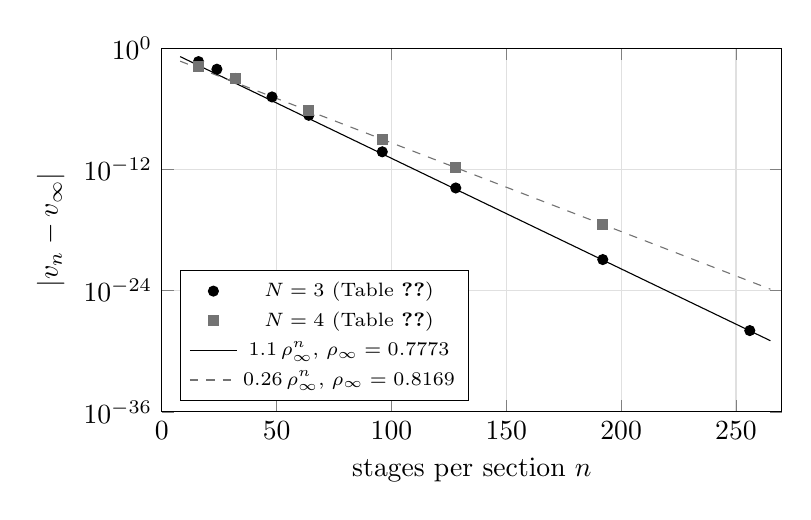
\begin{tikzpicture}
\begin{semilogyaxis}[width=0.78\textwidth,height=6.2cm,xlabel={stages per section \(n\)},ylabel={\(|v_n-v_\infty|\)},
  xmin=0,xmax=270,ymin=1e-36,ymax=1,legend pos=south west,legend style={font=\scriptsize},grid=major,grid style={black!12}]
\addplot[only marks,mark=*,mark size=1.8pt] coordinates {(16,4.67e-2) (24,8.22e-3) (32,9.87e-4) (48,1.48e-5) (64,2.25e-7)
  (96,5.48e-11) (128,1.44e-14) (192,1.18e-21) (256,1.10e-28)};
\addlegendentry{\(N=3\) (Table~\ref{tab:n3})}
\addplot[only marks,mark=square*,mark size=1.8pt,black!55] coordinates {(16,1.50e-2) (32,1.07e-3) (64,7.37e-7) (96,1.00e-9)
  (128,1.53e-12) (192,3.63e-18)};
\addlegendentry{\(N=4\) (Table~\ref{tab:n4})}
\addplot[domain=8:265,samples=60,thin] {1.1*0.7773^x};
\addlegendentry{\(1.1\,\rho_\infty^n\), \(\rho_\infty=0.7773\)}
\addplot[domain=8:265,samples=60,thin,dashed,black!55] {0.26*0.8169^x};
\addlegendentry{\(0.26\,\rho_\infty^n\), \(\rho_\infty=0.8169\)}
\end{semilogyaxis}
\end{tikzpicture}
\caption{Distance between the finite-stage steady state and the limit configuration (junction compositions and column
splits) against the number of stages per section, with the rate \(\rho_\infty\) predicted by Theorem~\ref{thm:perturbation}
(largest ratio of consecutive eigenvalues at the pinches of the limit configuration).}\label{fig:rate}
\end{figure}

\emph{Two illustrative cases} (Tables~\ref{tab:n3}--\ref{tab:n4}, Figure~\ref{fig:rate}). The distance to the limit
configuration decays like \(\rho_\infty^n\) with the predicted rate, the products \(1\) and \(N\) purify geometrically, the side
products tend to their designed impurities \(O(\eta)\), the smallest singular value of the finite-stage Jacobian tends to
that of the limit Jacobian, and \(R-\Hs=\delta\) exactly. Table~\ref{tab:approach} follows the order of limits of the proof:
as \((\delta,\eta)\to0\), the side-product impurity follows its designed value and \(R\to\Hs\), with stage numbers growing like
\(\log(1/\eta)\), since \(\sigma_{\min}(DG_\infty)\) is proportional to \(\eta\) in the product-form normalization.

\emph{A broader campaign.} The same solver was run on 62 cases: \(N=3\) with all four forcing patterns, \(q\) from \(-10\) to
\(10\), \(\alpha\) from \((1.05,1.02,1)\) to \((100,10,1)\), feed fractions down to \(10^{-4}\), two equal highest peaks, \(\delta\) down to
\(0.001\) and forcing up to \(0.95f_p\); \(N=4\) with all eight patterns, \(q\) from \(-5\) to \(6\), three equal peaks and close volatilities;
random instances for \(N=5\) to \(8\); \(n\) up to 768 (4000 for nearly equal volatilities); unequal section lengths with ratios up
to 8. In all 61 cases inside the admissible region, \(DG_\infty(v_\infty)\) is invertible with the block structure of
Theorem~\ref{thm:L}, every trace block reduces to a nonsingular M-matrix, and the finite-stage steady states are physical
and converge to \(\cL\) at the predicted rate. Without forcing, \(\sigma_{\min}(DG_n)\) decays geometrically
(\(8.2\cdot10^{-5}\), \(9.8\cdot10^{-7}\), \(1.4\cdot10^{-8}\) at \(n=16,24,32\) for \(N=3\)), while with forcing it stays near
\(0.007\): the neutral mode of Remark~\ref{rem:forcing}. The one failing case was chosen outside the admissible region on
purpose (a three-component case with \(\delta=0.002\) and a prefractionator slack \(0.05>\bar\eta(\delta)\), so that a binary margin is
negative): all algebraic hypotheses and the structure of Theorem~\ref{thm:L} hold, but a half-profile has a negative entry
and the zeros of \(G_n\) converging to \(v_\infty\) (\(n=32,64,128\)) have negative stage mole fractions
(Remark~\ref{rem:nonphysical}). The exact equations also have non-physical zeros far from \(\cL\) at admissible parameters.
Separately, the limit Jacobian was checked for 16 random instances with \(N=3\) to \(6\) (block structure exact, every trace row
as predicted by Lemma~\ref{lem:tracerow}), and the combinatorial case analysis of Theorem~\ref{thm:L} (rows, coordinates,
closed-to-open moves) was checked exhaustively for all \(N\le12\) and all \(2^{N-1}\) forcing patterns.

\emph{Independent re-implementations.} The two verifications of the attainment proof wrote their own codes from the
statements. The first built the design by solving its defining conditions, and the limit system from a general
eigen-solver instead of Underwood's formulas; on 23 cases (\(N=3\) to \(6\), all kinds of forcing patterns, forcing from
\(5\%\) to \(99.9\%\) of the bound \(\hat\eta_p\), nearly equal volatilities) it confirmed every property of
Theorem~\ref{thm:H}, the block structure of Theorem~\ref{thm:L} to finite-difference accuracy, and physical finite-stage
steady states with every unit balance satisfied to \(10^{-85}\). The second built the limit system from the explicit
Underwood and trace formulas, measured the constants of Lemma~\ref{lem:domain} and checked the inequalities of
Theorem~\ref{thm:perturbation} where they apply; it also observed that below \(n_0\) the zero of \(G_n\) closest to \(\cL\) need
not be physical (a three-component case with \(q=-0.5\) at \(n=16\)), while it is physical from \(n=32\) on, as the theorem
predicts. A deliberately broken version of the combinatorial check of Theorem~\ref{thm:L} (for example, unforced binary
columns) was detected in every mutation.

\emph{Earlier evidence.} The lower bound was checked on finite-stage steady states computed by four independent solvers
(random networks of up to twelve units with recycles, bypasses, split feeds, duties anywhere, products of either phase and
reverse net flows; columns and Petlyuk arrangements with up to 120 stages per section; Murphree trays), and its identities
in exact rational arithmetic; no violation was found. At fixed flows with a margin spread over all sections, three
independent solvers found the impurities of the three-component Petlyuk arrangement decreasing geometrically with \(n\),
which motivated the proof; with sharp binary columns their Jacobians showed the neutral mode.

\section{Discussion}\label{sec:discussion}

\emph{What is proved.} Within constant relative volatilities, constant molar flows, constant pressure, one feed, no heat
exchange between process streams and steady-state operation, every arrangement of equilibrium stages, single-phase
splitters and mixers, total condensers and vaporizers needs a total vaporization of at least \(\max_jH_j\) in the limit of
infinitely many stages and pure products (in fact \(R\ge H_j-c_j\varepsilon\) at every finite number of stages and purity
\(1-\varepsilon\)), and the generalized Petlyuk arrangement attains this value. This is the Halvorsen--Skogestad conjecture, read
as in Definition~\ref{def:conj}, together with their formula for the Petlyuk minimum, for every number of components. Both
halves were checked by independent verifiers who re-derived the proofs and re-implemented the constructions. The
lower bound is the stronger statement: it is uniform in the numbers of stages, holds at every steady state of every
arrangement (including non-adiabatic sections with external utilities and Murphree trays), and yields necessary conditions
for ties. The attainment is the more delicate one: it requires the order of limits \(n\to\infty\), then forcing \(\to0\), then
\(\delta\to0\), and gives no explicit stage numbers.

\emph{Scope and limitations.} (1)~\emph{Constant relative volatilities} enter the lower bound only through
Lemma~\ref{lem:uniform}: the vapor flux \(-(\theta v/S)G_x(\theta)\) has the sign of the liquid flux because \(y_i\propto\alpha_ix_i\).
For non-ideal mixtures this sign uniformity can fail, and the conjecture is open there (and not stated by its authors).
(2)~\emph{Constant molar overflow} enters only through the energy balance. Under the constant-heat-transport model
of~\autocite{MTA2023} (constant but component-dependent molar latent heats \(\lambda_i\), no sensible heat), the latent-heat
weighted flows \(\tilde n_{e,i}=\lambda_in_{e,i}\) satisfy the same balances, and the weighted compositions satisfy
\(\tilde y_i=\alpha_i\tilde x_i/\sum_k\alpha_k\tilde x_k\) again, so the lower bound extends verbatim, with the peaks of the
correspondingly weighted \(V_{\min}\) diagram; we have not examined attainment in that model. (3)~\emph{One feed}: with several
feeds the bound of Section~\ref{sec:consequences} holds, but it is not known whether it is attained, nor by which arrangement.
(4)~\emph{Internal heat exchange} is excluded by the conjecture, and Section~\ref{sec:consequences} shows why it must be: the
external heat can then fall below \(\Hs\), as in Halvorsen's examples~\autocite[Table~6.1]{HalvorsenThesis}; the minimum
external heat with heat integration (called unknown in~\autocite{HS02}) is not determined here. (5)~\emph{Steady state}:
periodic or batch operation is outside the model; with holdups, time-averaged outflows of a tray need not be
sign-uniform. (6)~\emph{Equilibrium stages}: devices that release streams of different compositions not in phase
equilibrium (decanters, membranes, component-specific efficiencies or mass-transfer rates) are outside \(\cA\) and outside the
conjecture's assumptions.

\emph{Relation to Underwood's model and to optimization.} Underwood's infinite-stage model remains the right tool to
\emph{compute} minimum vapor, and our results justify its value for the generalized Petlyuk arrangement. For global
optimization over configurations, Remark~\ref{rem:permissive} shows that relaxations of the model can return values below
\(\Hs\); the sign-consistency constraints derived from Lemma~\ref{lem:uniform} remove such points without removing physically
admissible excess vapor. The tie conditions of Section~\ref{sec:consequences} explain why many configurations reach the
Petlyuk value~\autocite{Jiang2018} and give necessary conditions for a configuration to do so.

\emph{Open questions.} (i)~Explicit stage numbers: the proof gives \(n_0\gtrsim\log(1/\eta)/\log(1/\rho_\infty)\) at fixed margins,
but no explicit constants; a quantitative version would turn the attainment into a design rule. (ii)~Uniqueness: we prove
local uniqueness near the limit configuration; whether the finite-stage Petlyuk network at the flows of
\(\cF(\delta,\eta,\pi)\) has a unique physical steady state is open (multiplicity is known for single columns under other
specifications~\autocite{JacobsenSkogestad1991}; uniqueness for binary columns with molar flow specifications goes back to
Rosenbrock, see~\autocite{DohertyPerkins1982}). (iii)~Which other arrangements attain \(\Hs\): the necessary conditions are
given here, sufficient conditions are not. (iv)~Non-ideal mixtures, several feeds, non-sharp products, and arrangements with
heat integration. (v)~A formal (machine-checked) proof: the lower bound is short enough for this; the attainment proof uses
analytic perturbation theory and would be a substantial formalization.

\section*{Data and code availability}

All scripts, logs and certificates are in the repository \texttt{chemistry-open-problems}, folder
\texttt{problems/halvorsen-skogestad-petlyuk-minimum-vapor/}; Appendix~\ref{app:repro} lists them with what each checks.
No result of this paper depends on a computation.

\section*{Use of artificial intelligence}

All mathematics, code and text of this work, including this manuscript and the literature review behind it, were produced
by AI agents (Claude Opus~5.5 and GPT-6-Astra), working under human direction in a structured workflow with separate
roles (solvers, red team, computation, independent verifiers). Every result was meant to be checked by an agent that had
not seen the solver's reasoning: the Underwood-model results were independently verified, the lower bound received an early
independent check (confirmed, with editorial corrections that are incorporated here), and the attainment proof was verified
independently by two further agents, one for the design and the limit system, one for the analysis and the integrated
proof (both confirmed it; the corrections were minor and editorial, and are incorporated here). Each verifier re-derived
the proofs by hand and re-implemented the construction in its own code. No human has checked the proofs line by line. Responsibility for any
submission of this work rests with the humans who submit it. The contributions are listed by role under the title.

\appendix
\renewcommand*{\thesection}{\Alph{section}}
\setcounter{section}{0}

\section{Two components: proof of Proposition~\ref{prop:binary}}\label{app:binary}

Take \(\alpha_1=\alpha>1=\alpha_2\), so \(\theta=\theta_1\in(1,\alpha)\) and \(H_1=(1-z)/(\theta-1)\). Write \(x,y\) for light mole
fractions and \(e(x)=\alpha x/(1+(\alpha-1)x)\) (increasing, strictly concave, \(e(0)=0\), \(e(1)=1\)). The column has a partial
reboiler (an (E) unit with duty \(s\), liquid product of composition \(x_B\)), \(n_B\) stages, a feed stage, \(n_T\) stages and a total
condenser (reflux and distillate of composition \(x_D\)); the flows are \(D=z\), \(B=1-z\), \(V_B=s\), \(V_T=s+1-q\),
\(L_T=V_T-D\), \(L_B=s+1-z\).

\emph{Flows.} \(H_1+1-q=\alpha z/(\alpha-\theta)>z\) by~\eqref{eq:feedroots}, so \(V_T>0\) and \(L_T>0\) for \(s\ge H_1\); and
\(H_1>(1-z)/(\alpha-1)\) since \(\theta<\alpha\).

\emph{Pinches.} The bottom map for a pure bottom product, \(\beta_0(x)=(s/L_B)e(x)\), has the fixed points \(0\) and
\(\hat x_B=(\alpha s/L_B-1)/(\alpha-1)\), which lies in \((0,1)\) because \(s(\alpha-1)>1-z\); and \(\beta_0(x)>x\) on \((0,\hat x_B)\) because
\(e(x)/x\) decreases. The downward top map for a pure top product, \(\tau_0(x)=e^{-1}((L_Tx+D)/V_T)\), has the fixed points \(1\)
and \(\hat x_T=(V_T/L_T-1)/(\alpha-1)\); between them the line \((L_Tx+D)/V_T\) lies below the concave curve \(e\), so \(\tau_0(x)<x\)
on \((\hat x_T,1)\). Now \(\hat x_T<\hat x_B\) if and only if \(f(s):=\alpha sL_T-V_TL_B>0\). Eliminating \(q\) with the feed equation
\(1-q=\alpha z/(\alpha-\theta)+(1-z)/(1-\theta)\), \(f\) is a quadratic in \(s\) with leading coefficient \(\alpha-1>0\) and roots \(H_1\) and
\(s_-=1/(\alpha-1)-z\theta/(\alpha-\theta)\), and
\[H_1-s_-=\frac{z\alpha(\theta-1)^2+(1-z)(\alpha-\theta)^2}{(\alpha-1)(\alpha-\theta)(\theta-1)}>0\]
(a two-line computation, checked symbolically). Hence \(s>H_1\) gives \(\hat x_T<\hat x_B<1\).

\emph{Shooting.} Fix \(\eta_1\in(0,1]\) with \(\eta_1\max(1,(1-z)/z)\le\varepsilon\). For \(\eta\in[0,\eta_1]\) put \(x_B=\eta\) and
\(x_D(\eta)=1-(1-z)\eta/z\in[1-\varepsilon,1]\) (light balance). Upward from the reboiler liquid,
\(x_0=\eta\), \(x_{k+1}=\beta_\eta(x_k):=(s\,e(x_k)+B\eta)/L_B\) (the balance \(sy_k-L_Bx_{k+1}=-Bx_B\)); after \(n_B+1\) steps this gives a
feed-stage liquid \(x^{\mathrm{bot}}_f(\eta)\). Downward from the condenser: the top-stage vapor has composition \(x_D\), each stage
has the liquid \(e^{-1}(y)\), and the vapor from the stage below is \(y_{\mathrm{next}}=(L_Tx+Dx_D)/V_T\) (the balance
\(V_Ty-L_Tx=Dx_D\)); after \(n_T+1\) stages this gives \(x^{\mathrm{top}}_f(\eta)\). All iterates stay in \([0,1]\), and both functions are
continuous in \(\eta\). If \(x^{\mathrm{bot}}_f(\eta)=x^{\mathrm{top}}_f(\eta)\), the two profiles form a steady state: every stage balance
holds by construction, the feed-stage balance is the difference of the two cross-section balances adjacent to it plus the
overall light balance \(Dx_D+Bx_B=z\), and the reboiler and condenser balances hold. At \(\eta=0\), \(x^{\mathrm{bot}}_f=0<1=x^{\mathrm{top}}_f\). Since \(\beta_{\eta_1}\ge\beta_0\) and both are increasing,
\(x^{\mathrm{bot}}_f(\eta_1)\ge\beta_0^{n_B+1}(\eta_1)\), which tends to \(\hat x_B\) (or is \(\ge\hat x_B\) if \(\eta_1\ge\hat x_B\)); since the
downward step with \(x_D(\eta_1)\le1\) is at most \(\tau_0\) and \(\tau_0\) is increasing,
\(x^{\mathrm{top}}_f(\eta_1)\le\max(\hat x_T,\tau_0^{n_T}(e^{-1}(x_D(\eta_1))))\), which tends to \(\hat x_T\). So for \(n_T,n_B\ge n_0\),
\(x^{\mathrm{bot}}_f(\eta_1)>(\hat x_T+\hat x_B)/2>x^{\mathrm{top}}_f(\eta_1)\), and the intermediate value theorem gives \(\eta^*\in(0,\eta_1)\)
with a steady state of purities \(1-\eta^*\) and \(1-(1-z)\eta^*/z\), both at least \(1-\varepsilon\), and \(R=s\). Every mole fraction of this steady state lies in \((0,1)\): \(x_B=\eta^*>0\) and
\(x_D\in(0,1)\); the upward step \(x\mapsto(s\,e(x)+B\eta^*)/L_B\) maps \((0,1)\) into \((0,1)\) because \(s\,e(x)+B\eta^*<s+B=L_B\); and the
downward step is a convex combination of points of \((0,1)\) followed by \(e^{-1}\), which maps \((0,1)\) onto itself. \qed

\section{One section and the exact reformulation}\label{app:section}

\begin{proof}[Proof of Lemma~\ref{lem:spectrum}]
(i) By the rank-one determinant formula, \(\det(\lambda-V\diag\alpha+w\alpha^\top)=\prod_i(\lambda-V\alpha_i)\bigl(1+\sum_i\alpha_iw_i/(\lambda-V\alpha_i)\bigr)\);
put \(\lambda=Vt\). At a root \(t\notin\{\alpha_i\}\) of \(P_w\), \(\Psi(t)=0\); \(P_w(\alpha_k)=-\alpha_kw_k\prod_{j\ne k}(\alpha_j-\alpha_k)\) vanishes if and only if
\(w_k=0\). (ii) For a root, \(\alpha\cdot\xi_\psi=V-\Psi(\psi)=V\), so \((M\xi_\psi)_i=V\alpha_i(\xi_\psi)_i-Vw_i=V\psi(\xi_\psi)_i\); for a trace mode
\(\alpha\cdot\xi_{\alpha_k}=(V-\Psi^{(k)}(\alpha_k))+\Psi^{(k)}(\alpha_k)=V\) and the same computation works (the \(k\)-th row uses \(w_k=0\)).
\((\ell^\top M)_j=V\alpha_j\ell_j-(\ell\cdot w)\alpha_j\) with \(\ell_\psi\cdot w=V\) for a root and \(\ell_{\alpha_k}\cdot w=w_k=0\) for a trace mode. For
\(\one^\top\xi_\psi\): \(\sum_iw_i/(\alpha_i-\psi)=\psi^{-1}\sum_iw_i\bigl(\alpha_i/(\alpha_i-\psi)-1\bigr)=\psi^{-1}(V-\one^\top w)=L/\psi\), and similarly
for a trace mode. Orthogonality and the values of \(\ell_\psi\cdot\xi_\psi\) follow from (iii). (iii) With
\(1/((\alpha-\psi)(\alpha-t))=\bigl(1/(\alpha-t)-1/(\alpha-\psi)\bigr)/(t-\psi)\), \(G_{\xi_\psi}(t)=\bigl((V-\Psi(t))-(V-\Psi(\psi))\bigr)/(t-\psi)\) for a
root; for a trace mode the sum over \(i\ne k\) gives \(-(\Psi^{(k)}(t)-\Psi^{(k)}(\alpha_k))/(t-\alpha_k)\) and the \(k\)-th term adds
\(\Psi^{(k)}(\alpha_k)/(\alpha_k-t)\). Then \(\ell_\chi\cdot\xi_\psi=G_{\xi_\psi}(\chi)=0\) for a root \(\chi\ne\psi\), and for a trace mode
\(\chi=\alpha_k\ne\psi\), \(\ell_\chi\cdot\xi_\psi=(\xi_\psi)_k=w_k/(\alpha_k-\psi)=0\). (iv) Distinct eigenvalues; \(\ell_\psi\cdot\hat\xi_\psi\ne0\) because
the modes are simple.
\end{proof}

\begin{proof}[Proof of Lemma~\ref{lem:onesigned}]
\(\Psi'(t)=-\sum_{i\in\Sigma}\alpha_iw_i/(\alpha_i-t)^2\) has constant sign. (a) Near \(a_j\) the term \(-\alpha_jw_j/(a_j-t)\) tends to \(-\infty\)
from the left and to \(+\infty\) from the right; \(\Psi(-\infty)=V\), \(\Psi(0)=V-\one^\top w=L>0\), and on \((a_1,\infty)\) every term
\(-\alpha_iw_i/(\alpha_i-t)\) is positive; monotonicity gives the roots. (b) The mirror image, with \(\Psi(+\infty)=V\).
\end{proof}

\begin{proof}[Proof of Lemma~\ref{lem:positive}]
(a) \(M=V\diag(\alpha)+|w|\alpha^\top\). (b) Sherman--Morrison, with \(1-\alpha^\top(V\diag\alpha)^{-1}w=1-\one^\top w/V=L/V\) and
\(\alpha^\top\diag(\alpha)^{-1}=\one^\top\). (c) \(M^k\hat\xi_\psi=(V\psi)^k\hat\xi_\psi\).
\end{proof}

\begin{proof}[Proof of Lemma~\ref{lem:analytic}]
Simple roots of a polynomial whose coefficients are analytic in \(w\) are analytic (implicit function theorem); simple real
roots stay real and keep their order; the spectral projectors \(\prod_{s\ne r}(M-\lambda_s)/(\lambda_r-\lambda_s)\) are analytic and of
rank one, which gives analytic \(\xi_r\), \(\ell_r\). For a trace mode write
\(P_w(t)=(\alpha_k-t)Q_w(t)-\alpha_kw_k\prod_{j\ne k}(\alpha_j-t)\) with \(Q_w(t):=\prod_{j\ne k}(\alpha_j-t)\Psi^{(k)}(t;w)\). At \(w^0\),
\(P_{w^0}=(\alpha_k-t)Q_{w^0}\), and simplicity of \(\alpha_k\) means \(Q_{w^0}(\alpha_k)\ne0\), that is \(\Psi^{(k)}(\alpha_k;w^0)\ne0\). Shrinking \(O\)
so that \(t_r(w)\) stays away from the \(\alpha_j\), \(j\ne k\), and \(\Psi^{(k)}(t_r;w)\ne0\), the equation \(P_w(t_r)=0\) divided by
\(\prod_{j\ne k}(\alpha_j-t_r)\) is~\eqref{eq:traceroot}. If \(w_k\ne0\), then \(t_r\ne\alpha_k\) and \(\tilde\ell_r=((\alpha_k-t_r)/\alpha_k)\,\ell_{t_r}\)
by~\eqref{eq:traceroot}, a left eigenvector by Lemma~\ref{lem:spectrum}; if \(w_k=0\), \(\tilde\ell_r=\bfe_k\), a left eigenvector by
Lemma~\ref{lem:spectrum}(ii). Formula~\eqref{eq:regtrace} is the definition written out, and the derivative follows because
\(t_r=\alpha_k\) where \(w_k=0\).
\end{proof}

\begin{proof}[Proof of Lemma~\ref{lem:productform}]
(a) \(\xt=cM^{n+1}\xb\) if and only if \(\ell_r\cdot\xt=c\lambda_r^{n+1}\ell_r\cdot\xb\) for all \(r\). Given this with \(c\ne0\), the index
\(r_*\) fixes \(c\); multiplying the relation of \(r\in U\) by \(\piv_{\mathrm{bot}}\lambda_{r_*}^{n+1}/\lambda_r^{n+1}\) and that of \(s\in D\) by
\(\piv_{\mathrm{bot}}\) gives \(E_r=0\), \(E_s=0\). Conversely, with \(c:=\piv_{\mathrm{top}}/(\lambda_{r_*}^{n+1}\piv_{\mathrm{bot}})\), \(E=0\) gives back every
relation. (b) Immediate. (c) The difference consists of terms \(\mu^{n+1}\times(\text{analytic})\), and
\(\nabla(\mu^{n+1})=(n+1)\mu^{n+1}\nabla\log\mu\). (d) Product rule at a zero.
\end{proof}

\begin{lemma}[weakly chained column-dominant Z-matrices]\label{lem:Mmatrix}
Let \(\mathfrak A=D-F\) be a square matrix with \(D=\diag(d_u)\), \(d_u>0\), \(F\ge0\) with zero diagonal, and nonnegative column sums
(\(d_u\ge\sum_{u'}F_{u'u}\) for every \(u\)). Call \(u\) \emph{leaky} if its column sum is positive, and suppose that from every index
\(u\) there is a chain \(u=u_0,u_1,\dots,u_\ell\) with \(F_{u_{t+1}u_t}>0\) ending at a leaky index. Then \(\mathfrak A\) is nonsingular,
\(\mathfrak A^{-1}\ge0\), and \((\mathfrak A^{-1})_{us}>0\) whenever there is a chain from \(s\) to \(u\) (in particular \(u=s\)).
\end{lemma}
\begin{proof}
Put \(P:=FD^{-1}\ge0\), so \(\mathfrak A=(I-P)D\) and the column sums of \(P\) are at most \(1\), with strict inequality exactly at the
leaky indices. The column sum of \(P^K\) at \(u\) is the mass left after \(K\) steps of the substochastic chain started at \(u\); it is
\(<1\) as soon as the chain can reach a leaky index within \(K-1\) steps. With \(K\) the number of indices, \(\|P^K\|_1<1\), so
\(\rho(P)<1\), \((I-P)^{-1}=\sum_kP^k\ge0\), and its \((u,s)\) entry is positive if a chain leads from \(s\) to \(u\). Finally
\(\mathfrak A^{-1}=D^{-1}(I-P)^{-1}\). (These are the weakly chained diagonally dominant matrices of~\autocite{ShivakumarChew1974};
see also~\autocite{BermanPlemmons}.)
\end{proof}

\begin{proof}[Proof of Proposition~\ref{prop:exact}]
(a) At a steady state all compositions lie in \(\cX\), so \(S\ge\alpha_N>0\). The component balances of the stages between a
cross-section and the bottom end of \(\sigma\) give \(V_\sigma y(x_k)-L_\sigma x_{k+1}=w_\sigma\) at every cross-section (\(0\le k\le n_\sigma\),
\(x_0:=\xb\), \(x_{n_\sigma+1}:=\xt\)), that is \(L_\sigma S(x_k)x_{k+1}=M_\sigma x_k\); iterating,
\(\xt=M_\sigma^{n_\sigma+1}\xb/\prod_k(L_\sigma S(x_k))\). The junction and product balances are \(b_c=f_c-d_c\) and the formula for \(\bar x_p\).

(b) Fix \(\sigma\) and drop the index. Since \(\one^\top M=L\alpha^\top\), \(\one^\top M^{k+1}\xb=L\,S(x_k)\,\one^\top M^k\xb\), so the iterates are
defined as long as \(S(x_k)\ne0\), \(x_{k+1}=Mx_k/(LS(x_k))\), and the cross-section balances \(Vy(x_k)-Lx_{k+1}=w\) hold for
\(0\le k\le n\). The hypothesis on \(\xt\) and \(\one^\top\xt=1\) give \(\xt=M^{n+1}\xb/(\one^\top M^{n+1}\xb)=x_{n+1}\), and the positive factor
is \(1/(L^{n+1}\prod_{k=0}^nS(x_k))\). The balance of stage \(k\) (\(1\le k\le n\)) is the difference of the cross-section balances
\(k-1\) and \(k\). The vapor entering stage \(1\) is that of the bottom-end node, of composition \(y(x_0)\); the liquid entering stage \(n\)
is that of the top-end node, of composition \(x_{n+1}\). At a node \(J\), by the end cross-section balances, the component balance
(out minus in) is \(\sum_{\bott(\sigma)=J}w_\sigma-\sum_{\topp(\sigma)=J}w_\sigma-(\text{feed})+(\text{product})\). At \(J_c\), \(c=[i,m]\), this is
\(d_c-b_{[i-1,m]}+b_c-d_{[i,m+1]}\) (minus \(z\) if \(c=[1,N]\)), that is \(d_c+b_c-f_c=0\). At \(J[p,p]\) it is
\(-d_{[p,p+1]}-b_{[p-1,p]}+P_p\bar x_p=0\). At the condenser, the top cross-section of \(\Ts[1,2]\) gives
\(Vy(x_n)=Lx_1+d_{[1,2]}=(L+P_1)\bar x_1=V\bar x_1\), so the condensed vapor has the composition \(\bar x_1\) of the reflux and of the
distillate, and the composition rule and the balance hold. Total and CMO balances hold by the specification, so the duties
are those of the specification.

\emph{Positivity.} Put \(K_{u,i}:=\alpha_i/S(x_u)>0\) at every unit \(u\) with a vapor outflow. For each component \(i\) the balances just
verified form a linear system \(\mathfrak A_i\,X_{\cdot,i}=z_i\,\bfe_{J[1,N]}\) in the vector of \(i\)-contents of all units, where
\(\mathfrak A_i\) has diagonal entries \(L_u+V_uK_{u,i}>0\) (total liquid and vapor outflows of \(u\), products included) and
off-diagonal entries \(-(\ell_{u'u}+v_{u'u}K_{u',i})\le0\) in column \(u'\), \(\ell_{u'u}\) and \(v_{u'u}\) being the liquid and vapor flows
from \(u'\) to \(u\). The column sum at \(u'\) equals the flow that \(u'\) sends to product outlets, and every unit is joined to a product node
along positive flows (liquid flows down every section and reaches the reboiler). By Lemma~\ref{lem:Mmatrix}, \(\mathfrak A_i\) is
nonsingular with a nonnegative inverse that is positive between units joined by a path of positive flows. Every unit is
reached from \(J[1,N]\) along positive flows, so \(x_{u,i}>0\) for every unit and every component, and \(y=Kx>0\) too.
\end{proof}

\section{The forced design: proofs}\label{app:design}

\begin{proof}[Proof of~\eqref{eq:feedfunction}]
Insert the definitions: \(\Psi_{\Ts[i,m+1]}-\Psi_{\Bs[i-1,m]}=V_{\Ts[i,m+1]}-V_{\Bs[i-1,m]}-\sum_k\alpha_k(d_{[i,m+1],k}+b_{[i-1,m],k})/(\alpha_k-t)=\Phi_{[i,m]}\),
and \(\Psi_{\Ts_c}-\Psi_{\Bs_c}=V_\Ts-V_\Bs-\sum_k\alpha_k(d_k+b_k)/(\alpha_k-t)=\Phi_c\) because \(d+b=f\) and \(V_\Ts-V_\Bs=U\).
\end{proof}

\begin{proof}[Proof of Lemma~\ref{lem:preferred}]
Partial fractions of \(\prod_r(t-\theta^c_r)/\prod_{p=i}^{m-1}(t-\alpha_p)=1+\sum_p\omega_p/(t-\alpha_p)\) give the formula for \(\Psi^0_\Ts\).
Numerator and denominator of \(\omega_p\) have \(p-i\) negative factors each, so \(\omega_p>0\), \(V^0_\Ts>0\) and \(d^0>0\). Since
\(\Psi^0_\Ts-\Psi^0_\Bs=\Phi_c\), \(\Psi^0_\Bs\) vanishes at every \(\theta^c_r\); since \(b^0_i=0\), \(\Psi^0_\Bs(t)\prod_{p=i+1}^m(t-\alpha_p)\) is a
polynomial of degree at most \(m-i\) with leading coefficient \(V^0_\Bs\) and the \(m-i\) roots \(\theta^c_r\); and \(V^0_\Bs=0\) would give
\(b^0=0\), contradicting \(b^0_m=f_m>0\). The residues give
\(-\alpha_pb^0_p=V^0_\Bs\prod_r(\alpha_p-\theta^c_r)/\prod_{p'\ne p}(\alpha_p-\alpha_{p'})\), of the sign of \(-V^0_\Bs\), and \(b^0_m>0\) forces
\(V^0_\Bs>0\). Finally \(L^0_\Ts=\Psi^0_\Ts(0)\) and \(L^0_\Bs=\Psi^0_\Bs(0)\) are positive by the product forms.
\end{proof}

\begin{proof}[Proof of Lemma~\ref{lem:slack}]
\(\theta^\star_c<\alpha_{i+1}\) and \(\theta^\star_c>\alpha_{m-1}\) by comparing the factors \(\theta^c_r\) with \(\alpha_{r+1}\) and \(\alpha_r\). \(K\) has
numerator and denominator of equal degree, leading coefficient \(1\) and simple poles at \(\alpha_{i+1},\dots,\alpha_{m-1}\) with residues
\(\alpha_ph_p\); \(K(0)=1\) by the choice of \(\theta^\star_c\), which gives \(\sum_ph_p=0\). At \(\theta^c_i\) and \(\alpha_i\) all factors are
positive; at \(\theta^c_{m-1}\) and \(\alpha_m\) numerator and denominator each have \(m-i-1\) negative factors.
\end{proof}

\begin{proof}[Proof of Definition~\ref{def:deformed} (the section functions)]
\(\Psi_{\Ts_c}=V^0_\Ts+\eta-\sum\alpha_p(d^0_p+\eta h_p)/(\alpha_p-t)=\Psi^0_\Ts+\eta K\), and with \(b=b^0-\eta h\),
\(\Psi_{\Bs_c}=V^0_\Bs+\eta+\sum\alpha_p(b^0_p-\eta h_p)/(\alpha_p-t)=\Psi^0_\Bs+\eta K\). Validity for \(m-i=2\) is immediate (\(h=0\)).
\end{proof}

\begin{proof}[Proof of Proposition~\ref{prop:deformed}]
(a) Lemma~\ref{lem:preferred} and \(\sum h=0\): \(L_\Ts=L^0_\Ts+\eta\), \(L_\Bs=L^0_\Bs+\eta\). (b) \(\Ts_c\) has \(w=d\ge0\) with support \([i,m-1]\)
and \(L_\Ts>0\): by Lemma~\ref{lem:onesigned}(a) it has one root in each \((\alpha_{p+1},\alpha_p)\), \(i\le p\le m-2\), and one in
\((0,\alpha_{m-1})\). \(\Psi_{\Ts_c}(\theta^c_r)=\eta K(\theta^c_r)=0\) for the middle \(r\); \(\Psi_{\Ts_c}(\theta^c_i)=\eta K(\theta^c_i)>0\), with
\(\Psi_{\Ts_c}\) decreasing on \((\alpha_{i+1},\alpha_i)\), gives \(r_c>\theta^c_i\); \(\Psi_{\Ts_c}(\theta^c_{m-1})>0\), with \(\Psi_{\Ts_c}\) decreasing on
\((-\infty,\alpha_{m-1})\), gives \(u_c>\theta^c_{m-1}>\alpha_m\) and \(\Psi_{\Ts_c}(\alpha_m)>0\). \(\Bs_c\) is symmetric (Lemma~\ref{lem:onesigned}(b),
\(\Psi_{\Bs_c}(\theta^c_i)>0\) and increasing). (c) Lemma~\ref{lem:spectrum} and (b). (d) Lemma~\ref{lem:spectrum}(ii):
\((\hat\xi^\Ts_u)_p=(u_c/L_\Ts)d_p/(\alpha_p-u_c)>0\) for \(p\le m-1\); \((\hat\xi^\Ts_{(m)})_p=(\alpha_m/L_\Ts)d_p/(\alpha_p-\alpha_m)>0\) (\(p<m\)) and
\((\hat\xi^\Ts_{(m)})_m=\Psi_{\Ts_c}(\alpha_m)/L_\Ts>0\); symmetrically for \(\Bs_c\). (e) \(G_X(t)\prod_{p\in[i,m]}(\alpha_p-t)\) is a polynomial of
degree at most \(m-i\) (exactly \(m-i\), with leading coefficient \(\pm S(X)\)); prescribing its \(m-i\) zeros fixes it up to a scalar,
the residues give the formula, and numerator and denominator of \(X_{c,p}\) have \(p-i\) negative factors each; the homogeneous
version gives the nonsingularity. In the eigenbasis of \(\Ts_c\), the coefficient of \(X_c\) on a major mode
\(\chi\in\{r_c,\theta^c_{\mathrm{middle}}\}\) is proportional to \(G_{X_c}(\chi)=0\), and on a trace mode \(\alpha_k\) (\(k\notin[i,m]\)) to
\(X_{c,k}=0\); so \(X_c=(1-\beta)\hat\xi^\Ts_{(m)}+\beta\hat\xi^\Ts_u\). By the pinch identity,
\(G_{\hat\xi^\Ts_{(m)}}(s_c)=-(\alpha_m/L_\Ts)\Psi_{\Ts_c}(s_c)/(s_c-\alpha_m)<0\) (\(\Psi_{\Ts_c}(s_c)>0\) since \(s_c<\theta^c_{m-1}<u_c\)) and
\(G_{\hat\xi^\Ts_u}(s_c)=-(u_c/L_\Ts)\Psi_{\Ts_c}(s_c)/(s_c-u_c)>0\); \(G_{X_c}(s_c)=0\) then forces \(0<\beta<1\). The bottom decomposition
is the same at \(r_c\).
\end{proof}

\begin{proof}[Proof of Proposition~\ref{prop:sharpbinary}]
\(V_\Ts=\kappa+\alpha_pf_p/(\alpha_p-\theta')>\alpha_pf_p/(\alpha_p-\theta')>f_p\) and \(V_\Bs=\kappa+\alpha_{p+1}f_{p+1}/(\theta'-\alpha_{p+1})>0\).
\(\Psi^0_\Ts\) decreases on \((-\infty,\alpha_p)\) with \(\Psi^0_\Ts(\theta')=\kappa>0\), and \(\Psi^0_\Bs\) increases on \((\alpha_{p+1},\infty)\) with
\(\Psi^0_\Bs(\theta')=\kappa>0\); their roots solve \(\alpha_p-t=\alpha_pf_p/V_\Ts\) and \(t-\alpha_{p+1}=\alpha_{p+1}f_{p+1}/V_\Bs\).
\end{proof}

\begin{proof}[Proof of Proposition~\ref{prop:Bforced}]
\(\hat\eta_p>0\) because \(\Psi^0_\Bs(\alpha_{p-1})>\kappa\) (Proposition~\ref{prop:sharpbinary}). (a) \(\one^\top d=f_p-\eta>0\), \(\one^\top b=f_{p+1}+\eta\),
\(L_\Ts=(V_\Ts-f_p)+\eta>0\), \(L_\Bs>0\). (b) \(\Psi_{\Ts_c}(t)=V_\Ts-\alpha_p(f_p-\eta)/(\alpha_p-t)\) vanishes at \(t=\alpha_pL_\Ts/V_\Ts\), which increases
with \(\eta\). (c) Lemma~\ref{lem:onesigned}(b) with poles \(\alpha_p,\alpha_{p+1}\): one root in \((\alpha_{p+1},\alpha_p)\) and one in
\((\alpha_p,\infty)\). On \((\alpha_{p+1},\alpha_p)\) the added term \(\alpha_p\eta/(\alpha_p-t)\) is positive, so \(\Psi_{\Bs_c}(\psi^0_\Bs)>0\) and
\(\psi''<\psi^0_\Bs\). Next, \(\psi'<\alpha_{p-1}\) if and only if \(\Psi_{\Bs_c}(\alpha_{p-1})>0\) (\(\Psi_{\Bs_c}\) increases on \((\alpha_p,\infty)\)), that is
\(\Psi^0_\Bs(\alpha_{p-1})-\alpha_p\eta/(\alpha_{p-1}-\alpha_p)>0\), which is the bound on \(\eta\). The trace modes are placed by
Lemma~\ref{lem:onesigned}(b). (d) \(\psi^\Ts\ge\psi^0_\Ts>\theta'\) and \(\psi^\Ts<\alpha_p\), so
\(\Psi_{\Bs_c}(\psi^\Ts)=\Psi^0_\Bs(\psi^\Ts)+\alpha_p\eta/(\alpha_p-\psi^\Ts)>\Psi^0_\Bs(\psi^\Ts)>\kappa\); as \(\Psi_{\Bs_c}\) increases on
\((\alpha_{p+1},\alpha_p)\), \(\Psi_{\Bs_c}(\psi^\Ts)>0\) is equivalent to \(\psi^\Ts>\psi''\). (e) Positivity: \(\psi'>\alpha_p>\alpha_{p+1}\). On the face
\(\{p,p+1\}\) the modes of \(\Ts_c\) are \(\psi^\Ts\) (vector \(\bfe_p\), since \(d\) is supported on \(\{p\}\)) and \(\alpha_{p+1}\) (left vector \(\bfe_{p+1}\)), and
\((\hat\xi^\Ts_{(p+1)})_{p+1}=\Psi_{\Ts_c}(\alpha_{p+1})/L_\Ts>0\) because \(\alpha_{p+1}<\psi^\Ts\) (Lemma~\ref{lem:onesigned}(a)). The coefficient of
\(\hat\xi^\Ts_{(p+1)}\) in \(X\) is \(X_{p+1}/(\hat\xi^\Ts_{(p+1)})_{p+1}>0\), and that of \(\bfe_p\) is \(G_X(\psi^\Ts)(\alpha_p-\psi^\Ts)/\alpha_p\), where
\(G_X(\psi^\Ts)=-(\psi'/L_\Bs)\Psi_{\Bs_c}(\psi^\Ts)/(\psi^\Ts-\psi')>0\) by (d) and the pinch identity. (f) Lemma~\ref{lem:analytic} with
\(k=p\): by~\eqref{eq:traceroot}, \(\psi'-\alpha_p=\alpha_p\eta/\Psi^{(p)}_{\Bs_c}(\psi')\to0\) with \(\Psi^{(p)}_{\Bs_c}=\Psi^0_\Bs\), so
\(\eta/(\psi'-\alpha_p)\to\Psi^0_\Bs(\alpha_p)/\alpha_p\).
\end{proof}

\begin{proof}[Proof of Proposition~\ref{prop:Tforced}]
The mirror image of Proposition~\ref{prop:Bforced}. \(\hat\eta_p>0\) since \(V_\Ts>f_p\) and \(\Psi^0_\Ts(\alpha_{p+2})>\kappa\).
\(\one^\top b=f_{p+1}-\eta>0\); \(L_\Ts>0\) by the bound (for \(p+1<N\) via Lemma~\ref{lem:onesigned}(a): \(\Psi_{\Ts_c}>0\) on
\((-\infty,\psi^{\mathrm{low}})\ni0,\alpha_{p+2}\)). \(\psi^\Bs\) solves \(t-\alpha_{p+1}=\alpha_{p+1}(f_{p+1}-\eta)/V_\Bs\); it exceeds \(\alpha_{p+1}\)
because \(f_{p+1}>\eta\) and decreases with \(\eta\). Lemma~\ref{lem:onesigned}(a) gives one root of \(\Psi_{\Ts_c}\) in \((\alpha_{p+1},\alpha_p)\) and one
in \((0,\alpha_{p+1})\); on \((\alpha_{p+1},\alpha_p)\) the added term \(\alpha_{p+1}\eta/(t-\alpha_{p+1})\) is positive, so \(\psi^{\mathrm{mid}}>\psi^0_\Ts\);
\(\psi^{\mathrm{low}}>\alpha_{p+2}\) if and only if \(\Psi_{\Ts_c}(\alpha_{p+2})>0\), which is the bound on \(\eta\). Margin: \(\psi^\Bs\le\psi^0_\Bs<\theta'\)
and \(\psi^\Bs>\alpha_{p+1}\), so \(\Psi_{\Ts_c}(\psi^\Bs)>\Psi^0_\Ts(\psi^\Bs)>\kappa\), and \(\Psi_{\Ts_c}\) decreases on \((\alpha_{p+1},\alpha_p)\). Cone:
\(G_X(\psi^\Bs)=-(\psi^{\mathrm{low}}/L_\Ts)\Psi_{\Ts_c}(\psi^\Bs)/(\psi^\Bs-\psi^{\mathrm{low}})<0\); the coefficient of \(\bfe_{p+1}=\hat\xi^{\Bs_c}_{\psi^\Bs}\)
is \(G_X(\psi^\Bs)(\alpha_{p+1}-\psi^\Bs)/\alpha_{p+1}>0\) and that of \(\hat\xi^\Bs_{(p)}\) is \(X_p/(\hat\xi^\Bs_{(p)})_p>0\), with
\((\hat\xi^\Bs_{(p)})_p=\Psi_{\Bs_c}(\alpha_p)/L_\Bs>0\) since \(\alpha_p>\psi^\Bs\). The limit \(\eta\to0\): Lemma~\ref{lem:analytic} with \(k=p+1\).
\end{proof}

\begin{proof}[Proof of Lemma~\ref{lem:balances}]
\emph{Feeds}: induction in the order of (F1); \(f_{[i,m]}=d_{[i,m+1]}+b_{[i-1,m]}\), where each parent contributes a vector positive
exactly on \([i,m]\) (validity), and a binary column is never a parent. \emph{Vapor at} \(J_c\): the outflows are \(V_{\Ts_c}\) and
\(V_{\Bs[i-1,m]}\), the inflows \(V_{\Bs_c}\) and \(V_{\Ts[i,m+1]}\); the difference is \(V_{\Ts_c}-V_{\Bs_c}-U_c=0\) (for \([1,N]\) the feed brings
\(1-q\)). \emph{Liquid at} \(J_c\): \(L_{\Bs_c}-L_{\Ts_c}=\one^\top d_c+\one^\top b_c-U_c=\one^\top f_c-U_c=L_{\Bs[i-1,m]}+q\,[c=[1,N]]-L_{\Ts[i,m+1]}\).
\emph{Side draws}: \(V_{\Bs[p-1,p]}=V_{\Ts[p,p+1]}\) by (F2) and \(L_{\Bs[p-1,p]}-L_{\Ts[p,p+1]}=\one^\top b_{[p-1,p]}+\one^\top d_{[p,p+1]}=P_p\).
Telescoping gives the vapors; summing \(d_c+b_c=f_c\) over the tree of columns gives \(\sum_p\bar n_p=z\).
\emph{Flux bookkeeping}~\eqref{eq:bookkeeping}: at \(J_c\) the left side is
\((V_{\Ts_c}-V_{\Bs_c}-U_c)-\sum_k\alpha_k(d_{c,k}+b_{c,k}-f_{c,k})/(\alpha_k-t)=0\) (for \(J[1,N]\): \(\varphi_F(t)\)); at a side draw,
\((V_{\Bs[p-1,p]}-V_{\Ts[p,p+1]})+\sum_k\alpha_k(b_{[p-1,p],k}+d_{[p,p+1],k}-\bar n_{p,k})/(\alpha_k-t)=0\); at the condenser,
\(-\Psi_{\Ts[1,2]}+\varphi_{P_1}=-V_{\Ts[1,2]}\); at the reboiler, \(\Psi_{\Bs[N-1,N]}+\varphi_{P_N}=V_{\Bs[N-1,N]}=R\). (This is
Lemma~\ref{lem:node} summed over the stages of each section.)
\end{proof}

\begin{proof}[Proof of Lemma~\ref{lem:middle}]
Induction top-down with~\eqref{eq:feedfunction}. For a valid parent deformed with \(\eta\ge0\), \(\Psi_\Ts=\Psi^0_\Ts+\eta K\) and
\(\Psi_\Bs=\Psi^0_\Bs+\eta K\), where \(\Psi^0_\Ts\), \(\Psi^0_\Bs\) vanish at all the parent's feed roots (Lemma~\ref{lem:preferred}) and \(K\) at
its middle ones (Lemma~\ref{lem:slack}); by induction these middle roots are global. So \(\Psi_{\Ts[i,m+1]}\) vanishes at
\(\theta_{i+1},\dots,\theta_{m-1}\) and \(\Psi_{\Bs[i-1,m]}\) at \(\theta_i,\dots,\theta_{m-2}\), hence \(\Phi_{[i,m]}\) vanishes at
\(\theta_{i+1},\dots,\theta_{m-2}\), and \(\Phi_{[i,m]}\) has exactly one root per interval. At \(\eta_{\mathrm{nb}}=0\) both section functions of
every non-binary column vanish at all of its feed roots, and the same induction makes every feed root of every column
global.
\end{proof}

\begin{proof}[Proof of Proposition~\ref{prop:margins}]
(a) (F1) involves neither \(R\) nor \(\eta_{\mathrm{bin}}\) nor \(\pi\). (b) \(V_{\Ts[p,p+1]}=R+\mathrm{const}\) (Lemma~\ref{lem:balances}), with
the constant and the binary feed independent of \(R\), and \(\kappa_p=V_{\Ts[p,p+1]}-\alpha_pf_p/(\alpha_p-\theta')\).

(c) (A light-side cut.) At \(\eta_{\mathrm{nb}}=0\) every feed root of every column is global (Lemma~\ref{lem:middle}); in particular
\(\theta_p\) is the feed root of \([p,p+1]\) and a root of \(\Psi_{\Ts[i,p+1]}\) for every non-binary \([i,p+1]\) (Lemma~\ref{lem:preferred}).
Since \(\kappa_p\) does not depend on \(\eta_{\mathrm{bin}}\), we may evaluate the identities~\eqref{eq:bookkeeping}, which are algebraic
consequences of the balances, with the sharp binary net flows (\(\eta_{\mathrm{bin}}=0\)), for which \(\bar n_r=z_r\bfe_r\) for every product
\(r\). Sum~\eqref{eq:bookkeeping} at \(t=\theta_p\) over the \emph{light} nodes: the junctions \(J[i,m]\) with \(m\le p\), the condenser
and the side draws \(J[2,2],\dots,J[p,p]\). A section with both ends light contributes \(\Psi-\Psi=0\); a bottom section
\(\Bs[i,m]\) with a light end has \(m\le p\), so both ends are light; a top section \(\Ts[i,m]\) with a light end has \(m\le p+1\); so the
sections with exactly one light end are the \(\Ts[i,p+1]\), \(1\le i\le p\), whose top end \(J[i,p]\) is light. The feed enters \(J[1,N]\),
which is not light. Hence \(-\sum_{i=1}^p\Psi_{\Ts[i,p+1]}(\theta_p)+\sum_{r=1}^p\varphi_{P_r}(\theta_p)=-V_{\Ts[1,2]}\). Summing~\eqref{eq:bookkeeping}
over all nodes, every section cancels and \(\sum_r\varphi_{P_r}(t)=R-V_{\Ts[1,2]}+\varphi_F(t)\) for every \(t\); letting \(t\to\infty\) gives
\(V_{\Ts[1,2]}=R+1-q\). With \(\Psi_{\Ts[i,p+1]}(\theta_p)=0\) for \(i<p\),
\(\varphi_{P_r}(\theta_p)=-\alpha_rz_r/(\alpha_r-\theta_p)\) and the feed equation,
\[\kappa_p(0;\delta)=\Psi_{\Ts[p,p+1]}(\theta_p)=R+(1-q)-\sum_{r\le p}\frac{\alpha_rz_r}{\alpha_r-\theta_p}=R-\sum_{r>p}\frac{\alpha_rz_r}{\theta_p-\alpha_r}=R-H_p=g_p+\delta .\]
(d) All data of every column are real-analytic in \(\eta_{\mathrm{nb}}\) near \(0\) (simple roots of the feed functions, rational
expressions with nonvanishing denominators) as long as the feeds remain positive; (V) is strict at \(\eta_{\mathrm{nb}}=0\)
(Lemma~\ref{lem:preferred}), and the binary feed roots are simple. So there is \(\eta_1>0\) such that on the cube
\([0,\eta_1]^{(N-1)(N-2)/2}\) all columns are valid and \(\kappa_p(\cdot\,;0)\) is \(C^1\); take \(C_1:=\max_p\max\|\nabla\kappa_p(\cdot\,;0)\|_1\)
over the cube and use the mean value theorem and (c).
\end{proof}

\begin{proof}[Proof of Theorem~\ref{thm:admissible}]
By Proposition~\ref{prop:margins}(b), (d), \(\kappa_p(\eta_{\mathrm{nb}};\delta)=\kappa_p(\eta_{\mathrm{nb}};0)+\delta\ge g_p-C_1\bar\eta(\delta)+\delta\ge g_p+\delta/2\).
Openness and analyticity: finitely many strict inequalities between analytic functions.
\end{proof}

\begin{proof}[Proof of Theorem~\ref{thm:H}]
(H1)--(H4) collect Lemma~\ref{lem:balances}, Propositions~\ref{prop:deformed}, \ref{prop:Bforced}, \ref{prop:Tforced} and
Theorem~\ref{thm:admissible}.

\emph{(H5) and the limit relations, type by type.} The mode lists are those of Proposition~\ref{prop:deformed}(c) (types 1, 2) and
Propositions~\ref{prop:Bforced}--\ref{prop:Tforced} (types 3--6), with distinct positive modes, so \(\rho_\sigma<1\). We use
\(\ell_\psi\cdot x=G_x(\psi)\) for a major mode and \(\ell_\psi\cdot x=x_k\) for a trace mode \(\alpha_k\).
Type 1: \(G_{X_c}(r_c)=G_{X_c}(\theta_r)=0\) by Proposition~\ref{prop:deformed}(e), \(X_{c,k}=0\) for \(k<i\), and the top end
\(X_{[i,m-1]}\) is supported on \([i,m-1]\).
Type 2: the bottom end \(X_{[i+1,m]}\) is supported on \([i+1,m]\); \(G_{X_c}(\theta_r)=G_{X_c}(s_c)=0\) and \(X_{c,k}=0\) for \(k>m\).
Type 3: \(X_c\) is supported on \(\{p,p+1\}\); the top end \(\bar x_p\) has \(\Maj(p)\subseteq\{p-1,p\}\) (\(\pi_p=\Bs\)).
Type 4: \(\bar x_{p+1}\) has \(\Maj(p+1)\subseteq\{p,p+1,p+2\}\); \(X_c=\hat\xi_{\psi'}\) is annihilated by \(\ell_{\psi''}\) (Lemma~\ref{lem:spectrum}(iii))
and has no component \(k>p+1\).
Types 5, 6: the mirror images (\(\Maj(p)\subseteq\{p-1,p,p+1\}\), \(\Maj(p+1)\subseteq\{p+1,p+2\}\)).

\emph{Pivots (H8).} At a junction the pivot of the section whose pinch vector appears in the cone decomposition is its
coefficient: \(\beta^\Ts_c\) (type 1), \(\beta^\Bs_c\) (type 2), \(\beta^\Ts_c\) (type 3), \(1\) (type 4), \(1\) (type 5), \(\beta^\Bs_c\) (type 6), all
positive. At the other end \(x\) (a product, or a child's junction for types 1--2), \(\supp x\) lies entirely on one side of the pinch:
for a top section every component of \(\supp x\) is lighter than \(\psi_*\) (type 1: \(\supp\subseteq[i,m-1]\), \(u_c<\alpha_{m-1}\); type 3:
\(\subseteq\{p-1,p\}\), \(\psi^\Ts<\alpha_p\); type 5: \(\subseteq\{p-1,p,p+1\}\), \(\psi^{\mathrm{low}}<\alpha_{p+1}\)), so \(G_x(\psi_*)>0\), and
\(\ell_{\psi_*}\cdot\hat\xi_{\psi_*}=(\psi_*/L)(-\Psi'(\psi_*))>0\) (\(\Psi\) decreasing); for a bottom section every component of \(\supp x\) is
heavier than \(\psi_*\) (type 2: \(\subseteq[i+1,m]\), \(v_c>\alpha_{i+1}\); type 4: \(\subseteq\{p,p+1,p+2\}\), \(\psi'>\alpha_p\); type 6:
\(\subseteq\{p+1,p+2\}\), \(\psi^\Bs>\alpha_{p+1}\)), so \(G_x(\psi_*)<0\) and \(\ell_{\psi_*}\cdot\hat\xi_{\psi_*}<0\). In both cases \([x]_{\psi_*}>0\).

\emph{(H6).} By the limit relations, \(\xb=[\xb]_{\psi_*}(\hat\xi_{\psi_*}+\sum_{\psi<\psi_*}\dots)\) and similarly at the top, which gives the
expressions of \(v^{\mathrm{bot}}_k\), \(v^{\mathrm{top}}_k\); they converge to \(\hat\xi_{\psi_*}\). Nonnegativity: going up a bottom section
(types 2, 4, 6), \(M\ge0\) (Lemma~\ref{lem:positive}(a)); going down a top section (types 1, 3, 5), \(M^{-1}\ge0\)
(Lemma~\ref{lem:positive}(b)). The two other directions start at a junction and use the cone decompositions with nonnegative
pinch vectors and Lemma~\ref{lem:positive}(c): going up \(\Ts_c\) from \(X_c\), type 1 uses
\(X_c=(1-\beta^\Ts_c)\hat\xi^\Ts_{(m)}+\beta^\Ts_c\hat\xi^\Ts_u\), type 3 uses \(X_c=(1-\beta^\Ts_c)\hat\xi^\Ts_{(p+1)}+\beta^\Ts_c\bfe_p\), and in type 5
\(X_c=\hat\xi_{\psi^{\mathrm{low}}}\) is an eigenvector; going down \(\Bs_c\) from \(X_c\), type 2 uses
\(X_c=\beta^\Bs_c\hat\xi^\Bs_v+(1-\beta^\Bs_c)\hat\xi^\Bs_{(i)}\), in type 4 \(X_c=\hat\xi_{\psi'}\) is an eigenvector, and type 6 uses
\(X_c=\beta^\Bs_c\bfe_{p+1}+(1-\beta^\Bs_c)\hat\xi^\Bs_{(p)}\). Hence \(M^{\pm k}x\ge0\), and \(M^{\pm k}x\ne0\) since \(M\) is invertible; with
positive pivots, \(v_k\ge0\) and \(\one^\top v_k>0\), and since \(\one^\top v_k\to\one^\top\hat\xi_{\psi_*}=1\), \(\inf_k\one^\top v_k>0\).

\emph{(H7).} \(x_{J,k}=0\) is part of the limit relations. The closed-at-bottom trace modes of Table~\ref{tab:types} are \(\alpha_k\) with
\(k<i\) (type 1; \(\supp X_c=[i,m]\)), \(k\le i\) (type 2; \(\supp=[i+1,m]\)), \(k<p\) (types 3, 5; \(\supp X_c=\{p,p+1\}\)), \(k<p\) (type 4;
\(\supp\bar x_{p+1}\subseteq\{p,p+1,p+2\}\)), \(k\le p\) (type 6; \(\supp\subseteq\{p+1,p+2\}\)); the closed-at-top ones are \(k\ge m\) (type 1;
\(\supp\subseteq[i,m-1]\)), \(k>m\) (type 2; \(\supp X_c=[i,m]\)), \(k\ge p+1\) (type 3; \(\supp\subseteq\{p-1,p\}\)), \(k>p+1\) (types 4, 6;
\(\supp X_c=\{p,p+1\}\)), \(k>p+1\) (type 5; \(\supp\subseteq\{p-1,p,p+1\}\)). In each case \(k\) is lighter (bottom) or heavier (top) than the
whole support, so every term of \(G^{(k)}_{x_J}(\alpha_k)=\sum_{i\in\supp}\alpha_ix_i/(\alpha_i-\alpha_k)\) is negative, respectively positive.
The components with nonzero net flow are \([i,m-1]\) (type 1), \([i+1,m]\) (2), \(\{p\}\) (3), \(\{p,p+1\}\) (4, 5), \(\{p+1\}\) (6); comparing with
the supports of the end compositions gives the last statement of (H7). Hence a closed-at-bottom trace of a top section is
lighter than every component with nonzero net flow, so \(\alpha_k\) exceeds every pole and \(\Psi_\sigma(\alpha_k)>V>0\)
(Lemma~\ref{lem:onesigned}(a)); a closed-at-top trace of a top section lies below its smallest root, where \(\Psi_\sigma>0\); a
closed-at-bottom trace of a bottom section lies above its largest root, where \(\Psi_\sigma>0\); a closed-at-top trace of a bottom
section lies below every pole, where \(\Psi_\sigma>V\) (Lemma~\ref{lem:onesigned}(b)); and \(\Psi^{(k)}_\sigma=\Psi_\sigma\) since \(w_k=0\).
Finally, for a junction \(X_c\), \(c=[i,m]\), and \(k\notin[i,m]\): if \(k<i\), \(\alpha_k\) is a trace mode of \(\Ts_c\) above its pinch (types 1, 3, 5),
closed at \(X_c\); if \(k>m\), \(\alpha_k\) is a trace mode of \(\Bs_c\) below its pinch (types 2, 4, 6), closed at \(X_c\).

\emph{(H8).} \(R\): Lemma~\ref{lem:balances}. Purities: \(\bar n_p=b_{[p-1,p]}+d_{[p,p+1]}\), whose entries other than \(p\) are \(\eta_{p-1}\)
(on \(p-1\), if \(\pi_{p-1}=\Bs\)) and \(\eta_p\) (on \(p+1\), if \(\pi_p=\Ts\)). Pivots: shown above.
\end{proof}

\section{The limit system: proof of Theorem~\ref{thm:L}}\label{app:limit}

Throughout, the parameters are admissible and \(v_\infty=\cL\). In this appendix the rows of \(G_\infty\) are divided by the
nonvanishing pivot product \(\piv_{\mathrm{bot}}\piv_{\mathrm{top}}\): the row of a mode \(r\) closed at the end \(J\) of \(\sigma\) is
\(\ell_r\cdot x_J/\ell_{r_*}\cdot x_J\). By Lemma~\ref{lem:productform}(d) this does not affect the invertibility of the derivative at
\(v_\infty\). Left eigenvectors are Underwood's \(\ell_\psi\) for major modes and the regularized \(\tilde\ell\) of
Lemma~\ref{lem:analytic} for trace modes.

\emph{Coordinates.} On \(\cV\) we use the affine coordinates of Table~\ref{tab:coords}; all other entries of \((d_c,X_c)\) are
dependent (\(\one^\top d_c=\Delta_{\Ts_c}\), \(\one^\top X_c=1\), \(b_c=f_c-d_c\) given the parents). The change of variables is affine,
triangular in the order of the columns (parents first) and invertible. A trace coordinate carries the index \(k\) of its
component; its value at \(v_\infty\) is \(0\).

\begin{table}[ht]
\centering\footnotesize\setlength{\tabcolsep}{3pt}
\caption{Coordinates on \(\cV\), column by column.}\label{tab:coords}
\begin{tabular}{@{}>{\raggedright}p{2.0cm}>{\raggedright}p{5.0cm}>{\raggedright}p{3.1cm}>{\raggedright\arraybackslash}p{3.5cm}@{}}
\toprule
column & trace coordinates & major coordinates & dependent\\
\midrule
non-binary \([i,m]\) & \(d_{c,k}\) (\(k\notin[i,m]\)), \(d_{c,m}\), \(b_{c,i}\); \(X_{c,k}\) (\(k\notin[i,m]\)) & \(d_{c,p}\) (\(i<p<m-1\)); \(X_{c,p}\) (\(i<p\le m\)) & \(d_{c,i}=f_{c,i}-b_{c,i}\), \(d_{c,m-1}\), \(X_{c,i}\)\\
binary, \(\pi_p=\Bs\) & \(d_{c,k}\) (\(k\ne p\)); \(X_{c,k}\) (\(k\notin\{p,p+1\}\)) & \(X_{c,p+1}\) & \(d_{c,p}\), \(X_{c,p}\)\\
binary, \(\pi_p=\Ts\) & \(d_{c,k}\) (\(k\notin\{p,p+1\}\)), \(b_{c,p}\); \(X_{c,k}\) (\(k\notin\{p,p+1\}\)) & \(X_{c,p+1}\) & \(d_{c,p}=f_{c,p}-b_{c,p}\), \(d_{c,p+1}\), \(X_{c,p}\)\\
\bottomrule
\end{tabular}
\end{table}

The rows are the \emph{major rows} (non-pinch major modes) and the \emph{trace rows of component \(k\)} (the trace mode \(\alpha_k\) of a
section \(\sigma\) with \(w^\infty_{\sigma,k}=0\)). For a component \(k\) let
\(\cJ_k:=\{J:x^\infty_{J,k}=0\}=\{J[i,m]:i<m,\ k\notin[i,m]\}\cup\{J[p,p]:k\notin\Maj(p)\}\). Every \(J\in\cJ_k\) has first index \(>k\)
(\(k\) is lighter than the node, \(J\in\cJ^<_k\)) or second index \(<k\) (\(J\in\cJ^>_k\)), and by (H7) every section attached to a node of
\(\cJ_k\) has zero limit net flow of \(k\).

\begin{lemma}[counts]\label{lem:counts}
For every column \(c\) and component \(k\), the trace rows of \(k\) carried by \(\Ts_c\) and \(\Bs_c\) are as many as the trace coordinates of
\(k\) of \(c\); the major rows of \(c\) are as many as its major coordinates (\(2(m-i-1)\) for a non-binary column, \(1\) for a binary one).
\end{lemma}
\begin{proof}
For \(k\notin[i,m]\): two trace rows (\(\Ts_c\), \(\Bs_c\)) and two coordinates (\(d_{c,k}\), \(X_{c,k}\)). Non-binary, \(k=i\): one row (\(\Bs_c\)),
one coordinate (\(b_{c,i}\)); \(k=m\): one row (\(\Ts_c\)), one coordinate (\(d_{c,m}\)); \(i<k<m\): none. Binary with \(\pi_p=\Bs\), \(k=p+1\): one
row (\(\Ts_c\)), coordinate \(d_{c,p+1}\); with \(\pi_p=\Ts\), \(k=p\): one row (\(\Bs_c\)), coordinate \(b_{c,p}\). Major rows: \(r_c\) and the
\(m-i-2\) middle modes in \(\Ts_c\), the middle modes and \(s_c\) in \(\Bs_c\); binary: \(\psi''\) or \(\psi^{\mathrm{mid}}\). Major coordinates:
\(m-i\) (in \(X_c\)) plus \(m-i-2\) (in \(d_c\)), or \(1\).
\end{proof}

\begin{lemma}[trace quantities are linear in the traces of their component]\label{lem:tracelinear}
Fix \(k\). For every section \(\sigma\) with \(w^\infty_{\sigma,k}=0\), \(w_{\sigma,k}(v)\) is a linear form in the trace coordinates of component
\(k\) only, and so is \(x_{J,k}(v)\) for every \(J\in\cJ_k\).
\end{lemma}
\begin{proof}
Induction over the columns, parents first: a \(d_{c,k}\) with \(d^\infty_{c,k}=0\) is a trace coordinate; a \(b_{c,k}\) with \(b^\infty_{c,k}=0\)
is either a trace coordinate (\(b_{c,i}\), \(b_{c,p}\)) or, for \(k\notin[i,m]\), \(d_{[i,m+1],k}+b_{[i-1,m],k}-d_{c,k}\) with both parental
limit flows zero (they are supported on \([i,m]\)). \(x_{J_c,k}=X_{c,k}\), and \(\bar x_{p,k}=(b_{[p-1,p],k}+d_{[p,p+1],k})/P_p\).
\end{proof}

\begin{lemma}[linearized trace rows]\label{lem:tracerow}
Let \(\alpha_k\) be a trace mode of \(\sigma\) closed at \(J\in\cJ_k\). With \(\nu^k_{J\to\sigma}\) the net flow of \(k\) from \(J\) into \(\sigma\)
(\(=w_{\sigma,k}\) if \(J=\bott(\sigma)\), \(=-w_{\sigma,k}\) if \(J=\topp(\sigma)\)) and
\(\gamma^{(k)}_\sigma:=|G^{(k)}_{x^\infty_J}(\alpha_k)|/\Psi^{(k)}_\sigma(\alpha_k)>0\) (by (H7)), the derivative at \(v_\infty\) of the row
\(\tilde\ell_k\cdot x_J/\ell_{r_*}\cdot x_J\) is
\(\bigl(\delta x_{J,k}-\gamma^{(k)}_\sigma\,\delta\nu^k_{J\to\sigma}\bigr)/\ell_{r_*}\cdot x^\infty_J\). In particular, at \(v_\infty\) the trace rows of
\(k\) depend only on the trace coordinates of \(k\).
\end{lemma}
\begin{proof}
By~\eqref{eq:regtrace} the numerator is \(x_{J,k}+w_{\sigma,k}\,g(v)\) with \(g\) analytic; \(x_{J,k}\) and \(w_{\sigma,k}\) vanish at \(v_\infty\), so
its derivative is \(\delta x_{J,k}+g(v_\infty)\,\delta w_{\sigma,k}\) with \(g(v_\infty)=G^{(k)}_{x^\infty_J}(\alpha_k)/\Psi^{(k)}_\sigma(\alpha_k)\); the
signs of (H7) (\(G^{(k)}<0\) at a bottom end, \(>0\) at a top end, \(\Psi^{(k)}>0\)) turn \(g\,\delta w\) into \(-\gamma\,\delta\nu\) at both kinds of ends.
Lemma~\ref{lem:tracelinear} gives the last statement.
\end{proof}

\begin{lemma}[node identities]\label{lem:nodeid}
For every component \(k\) and every node \(J\ne J[1,N]\), identically on \(\cV\),
\(\sum_{\sigma\text{ attached to }J}\nu^k_{J\to\sigma}(v)+P_Jx_{J,k}(v)=0\), with \(P_J:=0\) for a junction.
\end{lemma}
\begin{proof}
The junction balance \(d_c+b_c-f_c=0\) and the definition of \(\bar x_p\).
\end{proof}

\begin{proposition}[the trace blocks]\label{prop:traceblock}
For every \(k\), the square matrix \(\Tm_k\) of derivatives at \(v_\infty\) of the trace rows of \(k\) with respect to the trace
coordinates of \(k\) is nonsingular. More precisely, if \(\Tm_k\,\delta t=0\), the contents \(\zeta_J:=\delta x_{J,k}\) (\(J\in\cJ_k\)) solve
\(A_k\zeta=0\), where
\begin{gather*}
(A_k)_{JJ}=P_J+\sum_{\sigma\text{ closed at }J}\frac1{\gamma^{(k)}_\sigma},\\
(A_k)_{JJ'}=-\sum_{\sigma\text{ closed at }J',\text{ with open end }J}\frac1{\gamma^{(k)}_\sigma}\quad(J\ne J'),
\end{gather*}
and \(A_k\) is, after a permutation, upper triangular with positive diagonal: a nonsingular M-matrix.
\end{proposition}
\begin{proof}
Extend \(\delta t\) by zero to the other coordinates. By Lemma~\ref{lem:tracerow} every trace row of \(k\), of a section \(\sigma\) closed at
\(c(\sigma)\), gives \(\zeta_{c(\sigma)}=\gamma_\sigma\,\delta\nu_\sigma\) with \(\delta\nu_\sigma:=\delta\nu^k_{c(\sigma)\to\sigma}\). At \(J\in\cJ_k\) every
attached section has zero limit net flow of \(k\), hence \(\alpha_k\) as a trace mode, closed at one of its ends, and that end lies in \(\cJ_k\)
by (H7). The node identity (Lemma~\ref{lem:nodeid}, linear) gives
\(\sum_{\sigma\text{ closed at }J}\zeta_J/\gamma_\sigma-\sum_{\sigma\text{ open at }J}\zeta_{c(\sigma)}/\gamma_\sigma+P_J\zeta_J=0\) (at an open end the flow
into \(\sigma\) is \(-\delta\nu_\sigma\)), that is \(A_k\zeta=0\).
\emph{Triangularity.} If \(k\) is a lighter trace of \(\sigma\), then \(c(\sigma)=\bott(\sigma)\), the open end is \(\topp(\sigma)\), and
\(h(\topp)=h(\bott)-1\) (the top of \(\Ts[i,m]\) is \(J[i,m-1]\), the bottom of \(\Bs[i,m]\) is \(J[i+1,m]\)); if \(k\) is heavier,
\(c(\sigma)=\topp(\sigma)\) and \(h(\bott)=h(\topp)+1\); in both cases both ends lie in the same class \(\cJ^<_k\) or \(\cJ^>_k\). Ordering \(\cJ^<_k\)
by increasing \(h\) and then \(\cJ^>_k\) by decreasing \(h\), every nonzero off-diagonal entry lies above the diagonal.
\emph{Diagonal.} \(P_J>0\) at products; a junction \(J[i,m]\in\cJ^<_k\) is the closed bottom end of \(\Ts[i,m]\) for \(k\) (\(k<i\)), and
\(J[i,m]\in\cJ^>_k\) the closed top end of \(\Bs[i,m]\) (\(k>m\)), by (H7); and \(\gamma>0\). A triangular Z-matrix with positive diagonal is
a nonsingular M-matrix.
\emph{Conclusion.} \(\zeta=0\), hence \(\delta\nu_\sigma=0\) for every section with a trace row of \(k\); every trace coordinate of \(k\) is
some \(\zeta_J\) or \(\pm\) some \(\delta\nu_\sigma\) (Table~\ref{tab:coords}: a \(d_{c,k}\) or \(b_{c,k}\) with zero limit value is the net flow of
\(k\) in a section where \(\alpha_k\) is a trace mode), so \(\delta t=0\). \(\Tm_k\) is square by Lemma~\ref{lem:counts}.
\end{proof}

\begin{proposition}[the major block]\label{prop:majorblock}
Order the columns by decreasing length. The matrix \(\Mm\) of derivatives at \(v_\infty\) of the major rows with respect to the
major coordinates is block lower triangular over the columns, with nonsingular diagonal blocks \(\Mm_c\); hence \(\Mm\) is
nonsingular.
\end{proposition}
\begin{proof}
\emph{Triangularity.} The major rows of \(c\) are closed at \(J_c\) (Table~\ref{tab:types}) and depend on \(X_c\), \(d_c\) and \(f_c\), that is,
on the coordinates of \(c\) and of its ancestors.

\emph{Non-binary \(c=[i,m]\).} Let \(\delta\) be a variation of the major coordinates of \(c\) only, with \(\Mm_c\delta=0\). Then \(\delta f_c=0\) and
\(\delta d_{c,i}=\delta d_{c,m}=\delta d_{c,k}=0\) (\(k\notin[i,m]\)), so \(\delta d_c\) is supported on \(\{i+1,\dots,m-1\}\) with zero sum, and
\(\delta w_{\Ts_c}=\delta w_{\Bs_c}=\delta d_c\). For a root \(\chi\) of \(\Psi_{\Ts_c}\) or \(\Psi_{\Bs_c}\), \(\Psi'(\chi)\,\delta\chi=\mathcal R(\chi)\) with
\(\mathcal R(t):=\sum_p\alpha_p\delta d_p/(\alpha_p-t)\). Each major row is \(G_{X_c}(\chi)/(\text{pivot})\) with \(G_{X_c}(\chi)=0\), so its variation is
\([\ell_\chi\cdot\delta X_c+G'_{X_c}(\chi)\,\delta\chi]/(\text{pivot})\). The two rows of a middle root \(\theta_j\) (in \(\Ts_c\) and \(\Bs_c\)) give
\(G'_{X_c}(\theta_j)\,\mathcal R(\theta_j)\,(1/\Psi'_{\Ts_c}(\theta_j)-1/\Psi'_{\Bs_c}(\theta_j))=0\), where \(\Psi'_{\Ts_c}<0<\Psi'_{\Bs_c}\)
(Lemma~\ref{lem:onesigned}) and \(G'_{X_c}(\theta_j)\ne0\) (a simple zero of \(G_{X_c}\), Proposition~\ref{prop:deformed}(e)); so
\(\mathcal R(\theta_j)=0\) at the \(m-i-2\) middle roots, and \(\mathcal R(0)=\sum_p\delta d_p=0\). Then
\(\mathcal R(t)\prod_{p=i+1}^{m-1}(\alpha_p-t)\) is a polynomial of degree at most \(m-i-2\) with \(m-i-1\) distinct zeros, hence zero, and
\(\delta d_c=0\). (This is the invertibility of the Cauchy-type matrix \(\bigl(\alpha_p/(\alpha_p-\theta_j)\bigr)\) on \(\{\sum\delta d=0\}\).) Then
\(\delta\chi=0\) for every mode, and the rows of \(r_c\), the \(\theta_j\) and \(s_c\) say \(\ell_\chi\cdot\delta X_c=0\) at the \(m-i\) interlacing points,
with \(\sum\delta X_c=0\) and \(\delta X_c\) supported on \([i,m]\): \(\delta X_c=0\) by Proposition~\ref{prop:deformed}(e).

\emph{Binary \(c\), \(\pi_p=\Bs\).} The only major coordinate is \(X_{c,p+1}\) (with \(\delta X_{c,p}=-\delta X_{c,p+1}\)); the net flows and the
modes do not move, and the row of \(\psi''\) varies by
\(\bigl(\alpha_{p+1}/(\alpha_{p+1}-\psi'')-\alpha_p/(\alpha_p-\psi'')\bigr)\delta X_{c,p+1}/(\text{pivot})\ne0\), since \(\alpha_{p+1}<\psi''<\alpha_p\).
\(\pi_p=\Ts\): the same with \(\psi^{\mathrm{mid}}\in(\alpha_{p+1},\alpha_p)\).
\end{proof}

\begin{proof}[Proof of Lemma~\ref{lem:domain} and Theorem~\ref{thm:L}]
By (H5) and (H8) every section has \(N\) simple positive modes and nonzero pivots at \(v_\infty\); Lemma~\ref{lem:analytic},
continuity and Lemma~\ref{lem:productform}(c) give Lemma~\ref{lem:domain} (with \(n=\min_\sigma n_\sigma\), since
\(\bar\rho^{\,n_\sigma+1}\le\bar\rho^{\,n+1}\)), and \(G_\infty(v_\infty)=0\) is the set of limit relations of (H5)
(Lemma~\ref{lem:productform}(b)). The zero block and the block-diagonal form of \(\Tm\) follow from Lemma~\ref{lem:tracerow}; the
diagonal blocks are square by Lemma~\ref{lem:counts} and nonsingular by Propositions~\ref{prop:traceblock}
and~\ref{prop:majorblock}.
\end{proof}

\begin{example}[\(N=3\), pattern \((\Bs,\Ts)\)]\label{ex:N3}
Components A, B, C with volatilities \(a>b>c\); columns P \(=[1,3]\) (prefractionator), U \(=[1,2]\), W \(=[2,3]\); A is sent down
\(\Bs_{\mathrm U}\) into the side product and C up \(\Ts_{\mathrm W}\). The twelve coordinates are: for P, the trace flows
\(\varepsilon_{\mathrm C}:=d_{\mathrm P,C}\) and \(\varepsilon_{\mathrm A}:=b_{\mathrm P,A}\) and the major contents \(X_{\mathrm P,B},X_{\mathrm P,C}\); for U,
\(d_{\mathrm U,B}\), \(d_{\mathrm U,C}\) (traces), \(X_{\mathrm U,B}\) (major), \(X_{\mathrm U,C}\) (trace); for W, \(d_{\mathrm W,A}\), \(b_{\mathrm W,B}\),
\(X_{\mathrm W,A}\) (traces), \(X_{\mathrm W,C}\) (major). The rows, by section (modes in decreasing order, pinch marked \(*\)):
\(\Ts_{\mathrm P}\) (\(r_{\mathrm P},u^*_{\mathrm P},c\)): \(r_{\mathrm P}\) at \(J_{\mathrm P}\) (major) and \(c\) at \(J_{\mathrm U}\) (trace C);
\(\Bs_{\mathrm P}\) (\(a,v^*_{\mathrm P},s_{\mathrm P}\)): \(a\) at \(J_{\mathrm W}\) (trace A) and \(s_{\mathrm P}\) at \(J_{\mathrm P}\) (major);
\(\Ts_{\mathrm U}\) (\(\psi^{\Ts*},b,c\)): \(b\), \(c\) at the condenser (traces B, C);
\(\Bs_{\mathrm U}\) (\(\psi'^*,\psi'',c\)): \(\psi''\) at \(J_{\mathrm U}\) (major) and \(c\) at \(J_{\mathrm U}\) (trace C);
\(\Ts_{\mathrm W}\) (\(a,\psi^{\mathrm{mid}},\psi^{\mathrm{low}*}\)): \(a\) at \(J_{\mathrm W}\) (trace A) and \(\psi^{\mathrm{mid}}\) at \(J_{\mathrm W}\) (major);
\(\Bs_{\mathrm W}\) (\(a,b,\psi^{\Bs*}\)): \(a\), \(b\) at the reboiler (traces A, B).
No major coordinate enters a net flow (\(m-i-2=0\) for P), so \(\Mm=\diag(\Mm_{\mathrm P},\Mm_{\mathrm U},\Mm_{\mathrm W})\), where \(\det\Mm_{\mathrm P}\)
is, up to the pivots, the Underwood interpolation determinant
\(\det[\one^\top;\ (\alpha_k/(\alpha_k-r_{\mathrm P}))_k;\ (\alpha_k/(\alpha_k-s_{\mathrm P}))_k]\ne0\), and \(\Mm_{\mathrm U}\), \(\Mm_{\mathrm W}\) are the nonzero
scalars of Proposition~\ref{prop:majorblock}. The trace blocks reduce to
\begin{gather*}
A_{\mathrm A}=\begin{pmatrix}\gamma_{\Bs_{\mathrm P}}^{-1}+\gamma_{\Ts_{\mathrm W}}^{-1}&-\gamma_{\Bs_{\mathrm W}}^{-1}\\0&P_3+\gamma_{\Bs_{\mathrm W}}^{-1}\end{pmatrix},\qquad
A_{\mathrm C}=\begin{pmatrix}\gamma_{\Ts_{\mathrm P}}^{-1}+\gamma_{\Bs_{\mathrm U}}^{-1}&-\gamma_{\Ts_{\mathrm U}}^{-1}\\0&P_1+\gamma_{\Ts_{\mathrm U}}^{-1}\end{pmatrix},\\
A_{\mathrm B}=\diag\bigl(P_1+\gamma_{\Ts_{\mathrm U}}^{-1},\,P_3+\gamma_{\Bs_{\mathrm W}}^{-1}\bigr)
\end{gather*}
(nodes \(J_{\mathrm W}\), reboiler for A; condenser, reboiler for B; \(J_{\mathrm U}\), condenser for C; each \(\gamma\) is the coefficient of the
component of its block). So \(\det DG_\infty(v_\infty)\) is a product of explicit nonzero factors; the triangular solution starts at the
product nodes and moves to the junctions.
\end{example}

\section{From the limit system to steady states: proofs}\label{app:analysis}

\begin{lemma}[quantitative inverse function step]\label{lem:ift}
Let \(E\) be a finite-dimensional normed space, \(\mathcal G_\infty,\mathcal G\in C^1(\bar B;E)\) on \(\bar B:=\bar B(v_\infty,r_0)\),
\(\mathcal G_\infty(v_\infty)=0\), \(A:=D\mathcal G_\infty(v_\infty)\) invertible,
\(\Omega(r):=\sup_{|v-v_\infty|\le r}\|D\mathcal G_\infty(v)-A\|\), and \(r_1\in(0,r_0]\) with \(\|A^{-1}\|\,\Omega(r_1)\le1/4\). If
\(\sup_{\bar B}\|D\mathcal G-D\mathcal G_\infty\|\le1/(4\|A^{-1}\|)\) and \(\|A^{-1}\|\,|\mathcal G(v_\infty)|\le r_1/2\), then \(\mathcal G\) has exactly one zero
\(v^*\) in \(\bar B(v_\infty,r_1)\), and \(|v^*-v_\infty|\le2\|A^{-1}\|\,|\mathcal G(v_\infty)|\).
\end{lemma}
\begin{proof}
\(\Phi(v):=v-A^{-1}\mathcal G(v)\) has \(\|D\Phi(v)\|\le\|A^{-1}\|\bigl(\|A-D\mathcal G_\infty(v)\|+\|D\mathcal G_\infty(v)-D\mathcal G(v)\|\bigr)\le1/2\) on the
convex ball \(\bar B(v_\infty,r_1)\), which \(\Phi\) maps into itself:
\(|\Phi(v)-v_\infty|\le|\Phi(v)-\Phi(v_\infty)|+\|A^{-1}\|\,|\mathcal G(v_\infty)|\le r_1/2+r_1/2\). Banach's fixed-point theorem gives the unique zero,
and \(|v^*-v_\infty|\le|v^*-v_\infty|/2+\|A^{-1}\|\,|\mathcal G(v_\infty)|\).
\end{proof}

\begin{proof}[Proof of Theorem~\ref{thm:perturbation}]
On \(\cW\) (Lemma~\ref{lem:domain}), \(\sup\|DG_n-DG_\infty\|\le C_1\max_\sigma(n_\sigma+2)\bar\rho^{\,n_\sigma+1}\le C_1(n+2)\bar\rho^{\,n+1}\) for
\(n\ge1/\log(1/\bar\rho)\) (where \(x\mapsto(x+2)\bar\rho^{\,x+1}\) decreases), and \(|G_n(v_\infty)|=|(G_n-G_\infty)(v_\infty)|\le C_2\rho_\infty^{n+1}\) by
Lemma~\ref{lem:productform}(c) at \(w=w^\infty\) (every ratio \(\mu\) at \(v_\infty\) is at most \(\rho_\infty\)). \(G_\infty\) is analytic, so
\(\Omega(r)\le C_3r\). Take \(r_0\) with \(\bar B(v_\infty,r_0)\subset\cW\), \(r_1:=\min(r_0,1/(4C_3\|A^{-1}\|))\), and \(n_0\) with
\(C_1(n_0+2)\bar\rho^{\,n_0+1}\le1/(4\|A^{-1}\|)\) and \(\|A^{-1}\|C_2\rho_\infty^{n_0+1}\le r_1/2\), and apply Lemma~\ref{lem:ift} to
\(\mathcal G=G_n\). At \(v_n\) every section satisfies \(\xt=c_\sigma M_\sigma^{n_\sigma+1}\xb\) with \(c_\sigma\ne0\) (Lemma~\ref{lem:productform}(a)).
\end{proof}

\begin{lemma}[exact composite profile]\label{lem:profile}
At \(v_n\), take for a section \(\sigma\) the eigen-data at \(w_\sigma(v_n)\) with the right eigenvectors normalized by \(\one^\top\hat\xi_r=1\)
(possible near \(v_\infty\), since \(\one^\top\hat\xi^\infty_r=1\)) and the left eigenvectors rescaled so that \(\ell_r\cdot\hat\xi_r=1\) (so
\(\ell_r\cdot x=[x]_r\) and the pivots are \([\xb]_{r_*}\), \([\xt]_{r_*}\)); put \(a_s:=\ell_s\cdot\xb/\piv_{\mathrm{bot}}\) (\(s\in D\)) and
\(b_r:=\ell_r\cdot\xt/\piv_{\mathrm{top}}\) (\(r\in U\)). For \(0\le k\le n_\sigma+1\),
\begin{equation}\label{eq:profile}
u_k:=\frac{M^k\xb}{\piv_{\mathrm{bot}}\lambda_{r_*}^k}=\hat\xi_{r_*}+\sum_{s\in D}a_s\mu_s^k\hat\xi_s+\sum_{r\in U}b_r\mu_r^{n_\sigma+1-k}\hat\xi_r ,
\end{equation}
and the stage compositions of Proposition~\ref{prop:exact} are \(x_k=u_k/\one^\top u_k\).
\end{lemma}
\begin{proof}
\(M^k\xb=\sum_r(\ell_r\cdot\xb)\lambda_r^k\hat\xi_r\), and \(E_r=0\) (\(r\in U\)) gives \(\ell_r\cdot\xb=\mu_r^{n_\sigma+1}b_r\piv_{\mathrm{bot}}\).
\end{proof}

The profile is a bottom half-profile decaying upward plus a top half-profile decaying downward, glued at the pinch; at
\(v_\infty\) these are the \(v^{\mathrm{bot}}_k\) and \(v^{\mathrm{top}}_k\) of (H6).

\begin{lemma}[\(S>0\) at every stage]\label{lem:Spos}
Let \(c_0:=\min_\sigma\min(\inf_k\one^\top v^{\mathrm{bot}}_k,\inf_k\one^\top v^{\mathrm{top}}_k)>0\) (H6). There are \(n_1\ge n_0\) and \(C\) such that for
\(\min_\sigma n_\sigma=n\ge n_1\), every \(\sigma\) and \(0\le k\le n_\sigma+1\),
\begin{gather*}
|u_k-v^{\mathrm{bot}}_k|_\infty\le C(\rho_\infty^{n+1}+\bar\rho^{\,n_\sigma+1-k}),\qquad
|u_k-v^{\mathrm{top}}_{n_\sigma+1-k}|_\infty\le C(\rho_\infty^{n+1}+\bar\rho^{\,k}),\\
\one^\top u_k\ge c_0/2,\qquad S(x_k)\ge\frac{\alpha_Nc_0}{2\,\one^\top u_k}>0 .
\end{gather*}
\end{lemma}
\begin{proof}
The coefficients \(\hat\xi_r,\mu_r,a_s,b_r\) of~\eqref{eq:profile} are analytic in \(v\) on \(\bar B(v_\infty,r_1)\) and equal at \(v_\infty\) to those of
(H6), so they differ from them by at most \(C|v_n-v_\infty|\le C\rho_\infty^{n+1}\); since all \(\mu\le\bar\rho\),
\(|\mu^k-(\mu^\infty)^k|\le(\sup_jj\bar\rho^{\,j-1})|\mu-\mu^\infty|\) uniformly in \(k\). Comparing~\eqref{eq:profile} termwise with
\(v^{\mathrm{bot}}_k\), the \(\hat\xi_{r_*}\)- and \(D\)-terms differ by at most \(C\rho_\infty^{n+1}\), and the \(U\)-terms are at most
\(C\bar\rho^{\,n_\sigma+1-k}\) (\(b_r\) is bounded because \(|\piv_{\mathrm{top}}|\ge\piv_0\)); with \(v^{\mathrm{top}}_{n_\sigma+1-k}\), the \(U\)-terms differ by at
most \(C\rho_\infty^{n+1}\) and the \(D\)-terms are at most \(C\bar\rho^{\,k}\). Since \(\min(\bar\rho^{\,k},\bar\rho^{\,n_\sigma+1-k})\le\bar\rho^{\,(n+1)/2}\),
for every \(k\) one of the two half-profiles, \(v\ge0\) with \(\one^\top v\ge c_0\), satisfies \(|u_k-v|_\infty\le\varepsilon_n:=C(\rho_\infty^{n+1}+\bar\rho^{\,(n+1)/2})\).
Then \(\one^\top u_k\ge c_0-N\varepsilon_n\) and \(\alpha^\top u_k\ge\alpha_Nc_0-(\sum_i\alpha_i)\varepsilon_n\); take \(n_1\) with \(N\varepsilon_n\le c_0/2\) and
\((\sum_i\alpha_i)\varepsilon_n\le\alpha_Nc_0/2\), and note \(S(x_k)=\alpha^\top u_k/\one^\top u_k\).
\end{proof}

\begin{proof}[Proof of Theorem~\ref{thm:near}]
Theorem~\ref{thm:perturbation} gives \(v_n\); Lemma~\ref{lem:Spos} gives \(S>0\) at every stage and \(\one^\top u_k\ne0\), so the iterates of
Proposition~\ref{prop:exact}(b) are defined; \(S>0\) at the node compositions because they are affine in \(v\) and within
\(C\rho_\infty^{n+1}\) of points of \(\cX\), where \(S\ge\alpha_N\) (enlarge \(n_1\) so that \(S\ge\alpha_N/2\) there). Proposition~\ref{prop:exact}(b) gives a steady state with (i) and (iv)
(Lemma~\ref{lem:balances}); (ii) follows from Theorem~\ref{thm:perturbation} and (H8), since the product compositions are affine in \(v\);
(iii) from Lemma~\ref{lem:Spos}; (v) from Theorem~\ref{thm:perturbation} and Proposition~\ref{prop:exact}(a).
\end{proof}

\section{Computations and reproducibility}\label{app:repro}

No proof in this paper depends on a computation. The scripts below check identities, re-derive the constructions
independently, and test the statements numerically; paths are relative to the problem folder
\path{problems/halvorsen-skogestad-petlyuk-minimum-vapor/} of the repository. Environment: Linux (Fedora under WSL), Python~3.12
with \texttt{numpy}, \texttt{scipy}, \texttt{sympy}, \texttt{mpmath}, \texttt{python-flint}; one thread; runtimes from seconds to a few
minutes unless stated. Each certificate script prints PASS or FAIL for each claim.

\emph{Lower bound.}
\begin{itemize}
\item \path{total/network/scripts/unit_identities_exact.py} (exact rationals, \texttt{sympy}): Lemma~\ref{lem:uniform} symbolically
for \(N=2,\dots,6\); the summed node balance (the cut identity for an arbitrary set of units) on random unit graphs with recycles,
arbitrary subsets and rational \(\theta\).
\item \path{total/network/scripts/section_identity_exact.py} (exact rationals): identity~\eqref{eq:sectionflux} and the single change of
side per section, on 400 random stage-to-stage profiles with net flows of both signs.
\item \path{total/foundations/scripts/unitnet.py}, \path{total/sections/scripts/check_stage_cut.py},
\path{total/network/scripts/cut_bound_check.py}, \path{total/simulation/scripts/test_stage_bound.py} and
\path{test_section_sign.py}, \path{total/verification-early/scripts/vexact.py} and \path{vtests.py}: four independent
steady-state solvers; Theorem~\ref{thm:stage} and its identity on thousands of random networks and on columns and Petlyuk
arrangements; no violation.
\item \path{total/network/scripts/permissive_sign_path.py}: the light-to-heavy sign path of the point of
Remark~\ref{rem:permissive} (40 digits); \path{verification/krawczyk_certificate.py}: interval certificate of that point.
\end{itemize}

\emph{Attainment.}
\begin{itemize}
\item \path{total/sections/scripts/check_binary_attainment.py}: the quadratic of Appendix~\ref{app:binary} (\texttt{sympy}).
\item \path{attainment/design/scripts/check_design.py}: (H1)--(H8) and Propositions~\ref{prop:deformed}--\ref{prop:margins} on 240
random instances, \(N=3,\dots,7\), random patterns (high precision).
\item \path{attainment/limit/scripts/check_combinatorics.py}: the case analysis of Lemmas~\ref{lem:counts}--\ref{lem:nodeid} and
Proposition~\ref{prop:traceblock} (rows, coordinates, closed-to-open moves, triangularity), exhaustively for \(N\le12\) and all
\(2^{N-1}\) patterns (exact, integer arithmetic).
\item \path{attainment/limit/scripts/check_limit_jacobian.py} and \path{check_unforced.py}: the block structure of
Theorem~\ref{thm:L} on random instances, \(N=3,\dots,6\); singularity without forcing (Remark~\ref{rem:forcing}).
\item \path{attainment/analysis/scripts/check_analysis.py}: zeros of \(G_n\) with generic numerical eigen-data, every balance
re-checked with the actual streams, \(N=3,4,5\).
\item \path{attainment/computation/scripts/paper_tables.py} (Tables~\ref{tab:n3}--\ref{tab:approach}, about 5 minutes) and
\path{run_batch.sh}, \path{run_case.py}, \path{spurious_zeros.py}, \path{redteam_design.py}, \path{forcing_study.py},
\path{eta_dependence.py}, \path{unequal_lengths.py} (the 62-case campaign of Section~\ref{sec:numerics}).
\end{itemize}

\emph{Independent verification of the attainment proof.} \path{attainment/verification-DL/scripts/v1_independent.py} (own
construction of the design and of the limit system with a general eigen-solver, finite-difference Jacobians, finite-stage
steady states with every balance re-checked; 23 cases) and \path{mutate_combinatorics.py} (ten deliberately broken models,
all detected); \path{attainment/verification-A/scripts/v2_perturbation.py} (explicit Underwood and trace eigen-data,
constants of Lemma~\ref{lem:domain}, the inequalities of Lemma~\ref{lem:ift}, contraction, physical re-shooting) and
\path{v2_binary_prop10.py} (Appendix~\ref{app:binary}: identities in \texttt{sympy} and shooting for six data sets).

\emph{Underwood model.} \path{theory/scripts/run_theory_checks.sh} and \path{computation/scripts/run_certificates.sh}
(the Underwood-model statements, the enumeration of regular-column configurations and the multistart minimizations
mentioned in the introduction).

\paperreferences
\end{document}
